%%%%%%%%%%%%%%%%%%%%%%%%%%%%%%%%%%%%%%%%%%%%%%%%%%%%%%%%%%%%%%%%%%%%%%%%%%%%%%%%%%%%%%%%%%%%%%%%%%%%%
%
%   Version     : 2.0
%
%   Filename    : main.tex
%
%   Description : This is the main file for the LaTeX thesis proposal document template.
%                 The template is intended for use by MSCS students. 
%
%                It is assumed that you can learn how to use LaTeX on your own.
%                Please check/read the following online LaTeX book:
%
%                                 http://en.wikibooks.org/wiki/LaTeX
%     
%   Author      : Florante R. Salvador
%
%   Contributors: 1.  Karlo Campos 
%                     a. margin settings for DLSU thesis paper 
%   
%   Notes       : Please email florante.salvador@dlsu.edu.ph for comments, suggestions, ideas etc.
%
%   Reference:
%
%
%   History/Updates:
%      March 12, 2009 -- created version 1.0 for release to CSC701M (Methods of Research) students
%      May 30, 2009   -- updated Title page and Abstract for undergrad ST students
%
%      Feb 27, 2015 -- Created Version 2 (major overhaul): changed class to report, created a figures folder, 
%                               removed unnecessary packages, added new comments  based on Ethel Ong's slides
%
%      Feb 24, 2018 -- Created Version 3
%                   Reorganized the chapters, i.e., Chapter 3 is now Theoretical Framework and Chapter 4
%                      is now Research Methodology.
%                   Included the Research Ethics documents as Appendix A.
%
%%%%%%%%%%%%%%%%%%%%%%%%%%%%%%%%%%%%%%%%%%%%%%%%%%%%%%%%%%%%%%%%%%%%%%%%%%%%%%%%%%%%%%%%%%%%%%%%%%%%%%

%%%%%%%%%%%%%%%%%%%%%%%%%%%%%%%%%%%%%%%%%%%%%%%%%%%%%%%%%%%%%%%%%%%%%%%%%%%%%%%%%%%%%%%%%%%%%%%%%%%%%%%%%%%%%%%%%%%%%%%
%
%  Filename   : preamble.tex
%
%  Description: Preamble file to :
%               a. specify related packages
%               b. set margins, commands, etc.
%
%  Note       : Edit the margin settings for your own printer
%                  You may add your own commands, environments (it is assumed that you know what you're doing.)
%
%%%%%%%%%%%%%%%%%%%%%%%%%%%%%%%%%%%%%%%%%%%%%%%%%%%%%%%%%%%%%%%%%%%%%%%%%%%%%%%%%%%%%%%%%%%%%%%%%%%%%%%%%%%%%%%%%%%%%%%

%\documentclass[12pt,titlepage,onepage, letterpaper]{article}

\documentclass[12pt,titlepage,onepage, letterpaper]{report}


%
%-- specify related packages
%

%
% \usepackage[utf8x]{inputenc}
%

\usepackage{pdfpages}
\usepackage{float}
\usepackage{morefloats}

\usepackage{apacite}           %-- APA style citation 
                               %-- refer to http://www.ctan.org/tex-archive/biblio/bibtex/contrib/apacite/

%
%  \usepackage{ucs}
%

\usepackage{amsmath}           %-- American Math Society packages
\usepackage{amsfonts}
\usepackage{amssymb}
\usepackage{pdflscape}
% changed from lscape to pdflscape then recompile 

\usepackage{graphicx}          %-- graphicx package needed for including figures in JPG or PNG format
 
%
%\usepackage{graphics}          %-- graphics related package (this was commented out) use when image is in EPS format
%

\usepackage{verbatim}          %-- this package allows you to have multiple lines of comments by
                               %-- example:
                               %   \begin{comment}
                               %        ...your text here...
                               %   \end{comment}  

\usepackage{color}             %-- allows use of color with text
                               %-- example:  \textcolor{red}{This is the colored text in red.}

\usepackage{url}  %-- allows use of URLs example: \url{https:\ccs1.dlsu.edu.ph}


%
%-- set margins,  you may need to edit this for your own printer
%
\topmargin 0.0in
\oddsidemargin 0.0in
\evensidemargin 0.0in

\voffset 0.0in
\hoffset 0.5625in

\textwidth 5.75in
\textheight 8.5in


\parskip 1em
\parindent 0.25in

\bibliographystyle{apacite}            %-- use APA citation scheme

\hyphenation{ana-lysis know-ledge}     %-- LaTeX may not hyphenate correctly some words you use in your document
                                       %-- use \hyphenation to instruct LaTeX how to do it correctly, example above

\newcommand{\degree}{^{\circ}}         %-- use \newcommand to create your own "commands"
                                       %-- \newcommand works like the #define you learned in your COMPRO1 class

\newcommand{\etal}{et al.}


%\newcommand{\sinag}{\emph{Sinag}}
%\newcommand{\sinagtwo}{\emph{Sinag2}}

\newcommand{\figref}[1]{Figure \ref{#1}}
\newcommand{\appref}[1]{Appendix \ref{#1}}

%-- \newcommand{\Section}[1]{\section{#1}\setcounter{figure}{0}\setcounter{table}{0}}

%\newcommand{\shade}{\multicolumn{1}{|>{\columncolor[gray]{0.25}}c|}{}}
%\newcommand{\tableheader}[1]{\rowcolor{black}\color{white}{#1}}
%\newcommand{\cell}[2]{\multicolumn{1}{#1}{#2}}
%\newcommand{\definition}[2]{\textbf{\textit{#1}} --- #2}
%\newcommand{\itembit}[1]{\item \textbf{\textit{#1}}}
%\newcommand{\sgdef}[2]{\parbox[t][][t]{1.75in}{\textbf{#1}} \> \parbox[t][][t]{4.0in}{#2}\\\\}

%\newenvironment{sinagglossary}{\begin{flushleft}
%\begin{tabbing}
%\hspace{1.75in}\=\\}{\end{tabbing}\end{flushleft}}

\newcommand{\thestitle}[1]{{\Large \textsc{#1}}}


%---
%  \renewcommand{\thefigure}{\thesection.\arabic{figure}}
%  \renewcommand{\thetable}{\thesection.\arabic{table}}
%  \renewcommand{\contentsname}{Table of Contents}




                %-- includes LaTeX source file for the preamble 
\usepackage{epigraph}
\usepackage{csquotes}
\usepackage{dirtytalk}
\usepackage{tikz}
\def\checkmark{\tikz\fill[scale=0.4](0,.35) -- (.25,0) -- (1,.7) -- (.25,.15) -- cycle;} 

                                  %-- include packages, sets the margin sequence, and many more... 
                                  %-- your job: check if the settings are suitable for your own printer

\graphicspath{{figures/}}  %-- figures is the name of the folder containing images JPG or PN

\begin{document}

%%%%%%%%%%%%%%%%%%%%%%%%%%%%%%%%%%%%%%%%%%%%%%%%%%%%%%%%%%%%%%%%%%%%%%%%%%%%%%%%%%%%%%%%%%%%%%%%%%%%%%
%
%   Filename    : title_page.tex 
%
%   Description : This file will contain your Title Page.
%                 
%%%%%%%%%%%%%%%%%%%%%%%%%%%%%%%%%%%%%%%%%%%%%%%%%%%%%%%%%%%%%%%%%%%%%%%%%%%%%%%%%%%%%%%%%%%%%%%%%%%%%%

\begin{titlepage}
\centering


%-- **EDIT** the following line to indicate your thesis title
\thestitle{FireflyX: Designing Interactions for a Mobile Musical Learning Tool for Children}
% or Designing Interactions for a Mobile Musical Learning Tool for Children
% PROS and CONS: If we use the name of the app, it would seem like its an applied research and prototype heavy
% if we use the second title, it seems experimental and will rely on the user tests and interactions

\vspace{1.75cm}
A Partial Thesis\\
Presented to\\
the Faculty of the College of Computer Studies\\
De La Salle University Manila

\vspace{1.75cm}
In Partial Fulfillment\\
of the Requirements for the Degree of\\
%Master of Science in Computer Science
Bachelor of Science in Computer Science\\
\vspace{1.75cm}
by\\
%-- **EDIT** the following line to indicate your name 
\vspace{1cm}

ATO, Paolo Miguel B.   \\
GAMUTAN, Mart Henrick A.  \\
SALCEDO, Antoine Mikhael M.   \\
VALENCIA, Josh Cezar L.   \\


\vspace{1.75cm}
%-- **EDIT** the following line to indicate your adviser's name 
Jordan Aiko P. DEJA \\
Adviser

\vspace{1.75cm}
\today
\end{titlepage}
              %-- includes LaTeX source file for the Title Page 
                                  %-- your job: **EDIT THIS FILE ** to indicate your own title, name, and thesis adviser's name


%%%%%%%%%%%%%%%%%%%%%%%%%%%%%%%%%%%%%%%%%%%%%%%%%%%%%%%%%%%%%%%%%%%%%%%%%%%%%%%%%%%%%%%%%%%%%%%%%%%%%%
%
%   Filename    : abstract.tex 
%
%   Description : This file will contain your abstract.
%                 
%%%%%%%%%%%%%%%%%%%%%%%%%%%%%%%%%%%%%%%%%%%%%%%%%%%%%%%%%%%%%%%%%%%%%%%%%%%%%%%%%%%%%%%%%%%%%%%%%%%%%%

\begin{abstract}
% From 150 to 200 words of short, direct and complete sentences, the abstract 
% should be informative enough to serve as a substitute for reading the thesis document 
% itself.  It states the rationale and the objectives of the research.  

% In the final thesis document (i.e., the document you'll submit for your final thesis defense), the 
% abstract should also contain a description of your research results, findings, 
% and contribution(s).

This research explores the interaction among children learning through a playful mobile musical interface.  In using the innate playful nature of children, a sandbox environment will be implemented to supplement the experiences of learning music. We will design gestures that allows children to interact with a firefly model that represents different musical rudiments, such as rhythm, beat-rest patterns, notes, measures, and sections. This will be accomplished through the use of a human-centered design process of understanding children, and music teachers. The findings will guide the design and development of an iterative prototype that will repeatedly be tested by children. Continuous feedback through experiments and usability tests will allow us to discover what human factors are exhibited by children when doing music composition tasks.

%
%  Do not put citations or quotes in the abstract.
%

% Keywords can be found at \url{http://www.acm.org/about/class/class/2012?pageIndex=0}.  Click the 
% link ``HTML'' in the paragraph that starts with ''The \textbf{full CCS classification tree}...''.

\begin{flushleft}
\begin{tabular}{lp{4.25in}}
\hspace{-0.5em}\textbf{Keywords:}\hspace{0.25em} & Human Computer Interaction, Music Representation, Sandbox Environment, Gestural Input, Usability testing, User Interface Design
\end{tabular}
\end{flushleft}
\end{abstract}
                %-- this is the Abstract page
                                  %-- your job: **EDIT THIS FILE** to indicate your own abstract

\pagenumbering{roman}             %-- this will number pages as i, ii, iii, etc...
\setcounter{page}{2}

\tableofcontents                  %-- this command is used to generate the Table of Contents


\newpage
\listoffigures                    %-- this command is used to generate List of Figures

\newpage                       
\listoftables                     %-- this command is used to generate List of Tables

\newpage

\pagenumbering{arabic}            %-- this will number pages as 1, 2, 3, etc...
\setcounter{page}{1}              


%%%%%%%%%%%%%%%%%%%%%%%%%%%%%%%%%%%%%%%%%%%%%%%%%%%%%%%%%%%%%%%%%%%%%%%%%%%%%%%%%%%%%%%%%%%%%%%%%%%%%%
%
%   Filename    : chapter_1.tex 
%
%   Description : This file will contain your Research Description.
%                 
%%%%%%%%%%%%%%%%%%%%%%%%%%%%%%%%%%%%%%%%%%%%%%%%%%%%%%%%%%%%%%%%%%%%%%%%%%%%%%%%%%%%%%%%%%%%%%%%%%%%%%

%added by sir jd just for fun
\epigraph{Music is a science which must have determined rules. These rules must be drawn from a principle which should be evident, and this principle cannot be known without the help of mathematics. I must confess that in spite of all the experience which I have acquired in music by practicing it for a fairly long period, it is nevertheless only with the help of mathematics that my ideas became disentangled and that light has succeeded to a certain darkness of which I was not aware before.}{\textit{\citep{rameau1722traite}}}


\chapter{Research Description}
\label{sec:researchdesc}    %--note: labels help you with hyperlink editing (using your IDE)

 
\section{Overview of the Current State of Technology}
\label{sec:overview}

%Paragraph 1
Music has been known to be an effective learning companion for children \cite{mcintire2007developing}. 
It is an integral part of their lives helping them understand the different complexities of life. Several applications and technologies have been developed to help children throughout their learning journey \cite{roschelle2000changing}.

%Paragraph 2
Music can trigger many types of memories in children and can be used to engage with them at any time. This makes music play an important role in their education \cite{levinowitz1999importance}. On the other hand, computers and digital applications have become part of a child's daily life which can lead the child to be more productive in doing educational tasks. By utilizing these technologies, music can contribute towards the overall learning of the child in certain knowledge areas like science and mathematics \cite{zaranis2013using}.

%Paragraph 3
%music is a difficult field of study
Music is also a complex cultural phenomena making it difficult to study as it has a wide variety of theories to learn \cite{byrd2009studying}. 
%why is music difficult
One of the main reasons that makes it difficult is its many representations. Since music is considered as a form of art, composers have the freedom to make music in any way so that they can define it the way they want it to be \cite{byrd2009studying}. 

%Paragraph 4
The difficulty in teaching a child to learn music is on how to make it enjoyable for them, as the learning comes from them exploring various instruments at an early age \cite{ghazali2005minds}. This playful nature leads to them doing simple acts like singing and playing musical games which can serve as a foundation in giving them a basic idea on musical theories. Copying or repeating sound, enables children to learn from different sound sources, giving them a sense of some musical rudiments like rhythm and pitch \cite{mcpherson2015child}. 


%Paragraph 5
%name specific studies/systems for teaching music or mobile music or learning with music (name 2-3 siguro)-=][=--]
Multimedia Technology has been widely used in the education of students especially in the field of teaching music \cite{tong2016design}. Examples of these technologies include applications such as Musilla Musical School \cite{educationalappstore2017}, which is an application designed to teach the principles of music to children. Another is Sesame Street Makes Music \cite{educationalappstore2015}, which is an application designed to help children explore instruments, tempo, and musical creativity. However these applications pose further opportunities for lurning such as the limitations in accurate representations.
% However these applications have some gaps in the education such as the Musilla Musical School having a  thoroughly planned curriculum and some inaccurate representations of key musical concepts such as rhythm and melody. The Sesame Street Makes Music also has its gaps by having a limited song choice. (@mart Comment ni sir baka pwede ilagay yung gaps ng 2 apps na to sa rrl)

%http://journals.sfu.ca/onlinejour/index.php/i-jet/article/view/5686
% first app: https://www.educationalappstore.com/app/mussila-music-school
%second app: https://www.educationalappstore.com/app/sesame-street-makes-music

%Paragraph 6
%Guide ni sir:
%Teka baket sandbox bigla haha sana may discussion muna on samples of these approaches such as mnemonic, instructional and while some follow the sandbox approach….
There are many different approaches that help in learning. One common way is children attending traditional schools as they use the instructional approach of learning where there is a teacher guiding them throughout the process. Another approach which is mostly unconventional in schools is the use of mnemonics where relatable associations are used to remember complpex ideas \cite{putnam2015mnemonics}. Next is the sandbox approach where the child can playfully learn using a virtual sandbox environment on their own. Here, they discover by themselves the ideas by exploring and playing around the sandbox environment. We want to discover whether these technologies such as implementing a virtual sandbox environment can enable children to play, create and explore music.

%Paragraph 7
%what is the sandbox approach?
%what makes it sandbox environemnet
%name some notable learning sandbox environment: (use Scratch.... then cite niyo na paper nila Giselle)
%sandbox for math, sandbox for machine learning... other sandbox
The sandbox approach is implemented usually in a specific software platform. This provides control over the resources that the software or users can use \cite{prevelakis2001sandboxing}. Much like the literal sandbox where people can only use items inside it, such an environment allows users to only interact with what is provided to them \cite{goldberg1996secure}. An example of a notable learning sandbox environment is Scratch
% (cite scratch paper)
. It is a visual programming language developed to deal with the problem of learning programming for novices, especially younger users \cite{maloney2010scratch}. It uses the sandbox approach to assist young people learn how to think creatively, reason systematically \cite{kaleliouglu2014effects}.
Its implementation of the sandbox approach aids children in learning how to work successfully with others, and think ingeniously \cite{nodalo2019building}. Another notable learning sandbox environment is the Sonification Sandbox \cite{walker2003sonification}. It allows users to independently map several data sets to timbre, pitch, volume, and pan, with full control over the default, minimum, maximum, and polarity for each attribute \cite{walker2003sonification}. By using the features from Sonification Sandbox, we get to take advantage of these features.


%Paragraph 8
%meron bang sandbox for music?
%two options
% option1: there are. if there are discuss their gaps, and areas for improvement
% option2: if wala, or limited... then we have we want to discover if we can introduce the sandbox approach
%we mention Otomushi, what about otomushi?
OtoMushi, derived from its Japanese meaning where \textit{oto} means sound and \textit{mushi} means insect, is a platform for interacting with sound samples which is represented by insects developed by Andre (2010). Its sandbox environment allows a controlled canvass where users can mix virtual creatures applying scratching techniques to explore sound \cite{andre2010otomushi}. It allows users to record sound when they speak. A tangible sandbox environment surface called smartskin by \cite{rekimoto2002smartskin} lacked responsiveness and that the resolution of the graphics were bad. In later iterations, OtoMushi was implemented on the iPad. By implementing it this way, children can play with the tool as if it was a virtual sandbox environment. With this, a child's playfulness can be exploited by allowing them to play with the tool as much as they want.
%  This makes it prone to noise and static sounds which makes it ineffective.
% 音虫

%Paragraph 9
%what is our RQ?
%(RQ)How might we design a sandbox environment and a firefly model that will help children learn music in a playful manner
%objective general objective: This research aims to answer the following research question?
    Music has many complex properties that make it difficult to learn. Children are also difficult to teach because they have a shorter attention span and require many repetitions when teaching music \cite{may2013public}. Sandbox environments have been found to work on children since play is central to early childhood education and it also provides a safe yet playful environment suited for their learning \cite{bos2014learning, dalgarno2010learning}. There are many music applications across several platforms that help in teaching music to children but there are only few that incorporate a sandbox environment that helps in accompanying their learning. With all these the tools and environments, this study aims to delve into the design of an interaction that will help children learn through a playful mobile interface.

%--- the following example shows how to include a figure in PNG format
% \begin{figure}[t]                %-- use [t] to place figure at top, [b] to place at the bottom, [h] for here
%   \centering                    %-- use this to center the figure
%   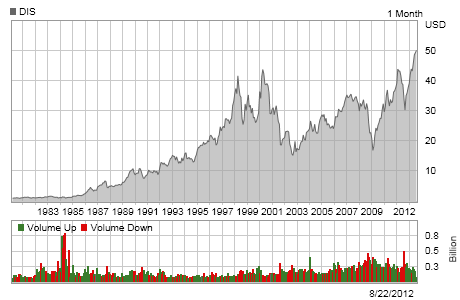
\includegraphics{DisneyChart.png}      %-- include image file named as "disneychart.png" 
%   \caption{This is the figure's caption -- Disney stock chart}
%     \label{fig:disneystock}
% \end{figure}


%
% Examples:
%     	Smith (1970) compared reaction times . . .
%     	In a recent study of reaction times (Smith, 1970), . . .   
%     	In 1970, Smith compared reaction times . . .
%	Smith, et al., (1970) compared reaction times . . .
%     	In a recent study of reaction times (Smith, et al., 1970), . . .  
%     	In 1970, Smith, et al., compared reaction times . . .
%

% Here are some examples on how to do the referencing (note author's name and years are different
% from commented examples).  For APA citation details, refer
% to \url{http://www.ctan.org/tex-archive/biblio/bibtex/contrib/apacite/}. 

% \begin{itemize}
%  \item \citeA{kartch:2000:ERA} compared reaction times...
%  \item In a recent study of reaction times \cite{kartch:2000:ERA}...
%  \item In \citeyearNP{kartch:2000:ERA}, \citeauthor{kartch:2000:ERA} compared reaction times...
%  \item \shortciteA{fedkiw:2001:VSO} compared reaction times... 
%  \item In a recent study of reaction times \cite{fedkiw:2001:VSO}...
%  \item In \citeyearNP{fedkiw:2001:VSO}, \shortciteauthor{fedkiw:2001:VSO}, compared reaction times...
% \end{itemize}

% The following are references from journal articles \cite{Park:2006:DSI, Pellacini:2005:LAH, 
% sako:2001:SSB}.  Here's an MS thesis document \cite{yee:2000:SSA}, and this is from
% PhD dissertation \cite{kartch:2000:ERA}. For a book, reference is given as 
% \cite{parke:1996:CFA}.  Proceedings from a conference samples are \cite{Jobs95, fedkiw:2001:VSO,
% levoy:2000:TDM}.  The sample bibliography file named \textbf{myreferences.bib} is from the
% SIGGRAPH \LaTeX template.  You can use a text editor to view the contents of the bib file.  
% It is your task to create your own bibliography file.  For those who downloaded papers from
% ACM or IEEE sites, there is a BibTeX link that you can click; thereafte   r, you just simply need
% to copy and paste the BibTeX entry into your own bibliography file.



% The following shows how to include a program source code (or algorithm).  The verbatim environment,
% as the name suggests, outputs text (including white spaces) as is...

% \begin{verbatim}
%               #include <stdio.h>
%               main()
%               {
%                     printf("Hello world!\n");
%               }
% \end{verbatim}


% \textcolor{red}{DO NOT FORGET to write the statement of the research problem here, i.e.,
% before the Research Objectives.}


\section{Research Objectives}
\label{sec:researchobjectives}

\subsection{General Objective}
\label{sec:generalobjective}

% To design a sandbox environment and a firefly model which is a firefly with different parts that represent different musical elements that will help children learn music in a playful manner.

This study aims to identify and model the human factors and behaviours that children exhibit when given the task of learning how to compose music with a mobile musical tool.

\subsection{Specific Objectives}
\label{sec:specificobjectives}

%
%  \begin{comment} ... \end{comment} is used for multiple lines of comment
%

\begin{comment}

This subsection is an elaboration of the general objective.  It states the specific steps that must be undertaken to accomplish the
general objective.  These objectives must be specific, measurable, attainable, realistic, time-bounded.  Each specific objective may
start with ``to design/survey/review/analyze''

Studying a particular programming language or development tool (e.g., to study Windows/Object-Oriented/Graphics/C++ programming) to 
accomplish the general objective is inherent in all thesis and, therefore, must not be included here.


%
% IPR acknowledgement: the following sentences and examples are from Ethel Ong's slides 
%     on Research Objectives
%

How to formulate your research objectives:
1. Identify what research steps do you need to perform to achieve your general objective.
2. Identify the questions that must be answered for you to achieve your general objective.
    Thereafter, convert these questions into action statements


Example #1:

Research Question:
  What are the general features of a web-based learning environment?

Specific Objective:
   To review existing web-based learning environment that teaches language learning for children


Example #2:

Research Question:
   How will you represent commonsense knowledge for use by computer systems?

Specific Objective:
   To identify knowledge representation approaches used by existing story generation systems

Example #3:
Research Question:
   What types of storytelling knowledge are needed to generate stories?

Specific Objective:
    To identify the different types of storytelling knowledge used in generating stories

Example #4:
Research Question:
    What machine learning approaches will you utilize?

Specific Objective:
    To determine existing machine learning algorithms [that can be used in training the computer system to detect cyberbullying cases] 

Example #5: Research Question:
    How will your research output be evaluated?

Specific Objective:
    To define evaluation metrics for validating the accuracy of the translation

\end{comment}

%
%  The following are example specific objectives; replace them with your own 
%
This research shall attempt to answer the following specific questions:
\begin{enumerate}
%   \item To design a sandbox environment where children can interact with firefly models.
%   \item To design a firefly model that will represent musical features playable by children.
%   \item To integrate the sandbox environment and firefly model in a mobile application.
%     \item To evaluate the usability of the sandbox environment, and the firefly models in terms of helping children learn music.
\item What activities do music teachers implement when teaching children music patterns?
\item What features can be designed to enable playful interactions when teaching children music?
\item What human factors do children exhibit when using the firefly and sandbox model?
\end{enumerate}


\section{Scope and Limitations of the Research}
\label{sec:scopelimitations}

    FireflyX is a virtual mobile music environment that will be developed on the iOS platform as a tablet application. With the use of the application, children can create their own music in an environment without the fear of breaking anything. The canvas will be able to house up to 5 virtual firefly models which can simultaneously produce sound making the environment multi-melodic when they are released. It will only provide what is needed by the children namely starting the composition, composing the rhythm,pitch and tempo by configuring the firefly model, and playing the composition in the environment with the other created fireflies. We would be observing the children based on how they are taught musical theories and our research will include students from different schools and their music classes.
    
    The firefly model will have a set musical features attached to its corresponding parts. These “movable” parts include the body, wings, and tail. Through the different parts of the firefly, children can configure the music through the use of interchangeable firefly model parts. These parts represent different musical rudiments of rhythm like clap-rest pattern, speed of sustain, and number of repetitions. It will also represent pitch and tempo as well. The firefly model can also represent one instrument and the target instrument for music creation is the piano due to its popularity with children. One firefly will represent one layer of the rhythm, pitch and tempo also for this model music filters will not be included. Dotted notation will not be included as well. The 4/4 time signature will only be the used by all firefly models. When the children are done manipulating the parts of the firefly model, the firefly model is released and the sound is created by the combination of the parts is played.
    
    The interactions the children will be limited to touch gestures that the mobile platforms can handle. Several touch gestures will be incorporated in the design to enable the children to play with the virtual firefly model. Such gestures include tap, drag, swipe, and flick. The target users of the application are children from ages 5-8. To evaluate the usability of the application the group will be evaluating the learning of children by giving them a set of instructions. After giving the instructions, we will be asking the music expert to evaluate the performance of the child. We will also be observing children use the app and assess the app’s usability afterwards.

\begin{comment}

%
% IPR acknowledgement: the sentences inside this comment are from Ethel Ong's slides on Scope and Limitations of the Research
%
Generally, one paragraph should be allotted for each of your research objectives.

Each paragraph contains a brief overview of the concept/theory and the purpose of doing the associated objective.

Each paragraph also includes a description of the scope/limitation of your study.

* Please refer to the slides for examples.

\end{comment}
    

\section{Significance of the Research}
\label{sec:significance}

This study attempts to design a usable mobile musical learning tool for children that incorporates computer-aided creativity, music elements and many others which can help children users to learn music theories at a young age. Additionally, the function of this tool will contribute in creating a child friendly interface for children to learn a hard concept like music. 

This tool will help children learn music through the sandbox interface that the application presents. The study helps to offer other music application developers an idea on how to design sandbox environments and integrate them into music learning.

Development of tools like this would give a basis for instructional designers to develop mobile products on what to do and what not to do when designing and developing these kinds of applications. What this study can offer can be set as a benchmark on what the quality of these products when they will release onto the public would be.

%
% IPR acknowledgement: the following list of items are from Ethel Ong's slides on Significance of the Research
%
% \begin{itemize}
% \item  What is the relevance of your work to the computer science community? 

% \begin{itemize} 
% \item What will be your technical contributions, in terms of algorithms, or approaches, or new domain? 
% \item What is your value-added compared to existing systems? 
% \end{itemize}

% \item What will be your contributions to society in general? 
%     \begin{itemize}
%       \item Who will benefit from your system? 
%       \item Who are your target users and how will this system benefit them? 
%   \end{itemize}
% \end{itemize}

% \begin{comment}
% If applicable, describe possible commercialization and/or innovation in your research.
% \end{comment}
\begin{comment}
\section{Research Methodology}
This chapter discusses the activities and specific steps that was done in this research. It also includes the the activities from thesis proposal to final thesis defense.

\subsection{Planning}
In this phase it shows the formulation of the thesis topic with the research problems and objectives, including the scope and limitation with the help of the thesis adviser. This also includes the planning of the future steps to do and what the output of the research is.

\subsection{Review of Related Literature}
Relevant works on Computer-Aided Instruction (CAI), Sandbox environments, and similar software's are being read and studied by the group to give the needed understanding to conduct the study. Works about Computer-Aided Instruction are important to the study as they provide an idea on how past applications have aided people in learning. Works on Sandbox environments will also be reviewed as they provide an idea on how we can implement the virtual environment that is suitable to the learning of the children and also how to test the usability of the said environment. Finally, works on similar software will also be reviewed to give context on how to make the tool usable and enjoyable for use of the children.

\subsection{Data Collection}
In this phase, the group will research on music theory and concepts. The information gathered there will be used for building the model for the musical representation of the tool. The group will also ask music experts on how to best evaluate children on their learning, as it is important to get their opinions on how to properly evaluate the children.

\subsection{Interaction Design}
This phase is concerned on building the experience that the users have with the application and listing down the steps on how it would help them. This part will also include on deciding on the user interface elements, and also how the users will interact with these elements. The data gathered from the group observing the users during testing will give good insight on what design elements we are good and what else we can improve on. The group will be making artifacts and user personas to represent the users, as this will be used in validating throughout different tests. All of these are to be done to make sure that we would integrate the solution to help in the learning of children. 

\subsection{Implementation}
In the implementation of the system, it will be a mobile application on the iOS platform. We chose IOS because IOS offers a less variety of screen sizes making it easier to design applications for. For the ease of use of the children it will be focused for the iPads, as it will be easier for them to interact with it due to iPads having a larger screen size than regular phones. As stated in the interaction design we will use the data gained from the observation throughout the different iterations of testing to further improve the implementation of the system.
    
\subsection{Testing}
To asses the effectiveness of the system that was developed, through out the research many iterations of testing will be done. These experiments will be designed to measure two things the first is the overall learning of the children and second is to measure the user experience and the interaction they have with it. We will use user experience metrics to help asses the overall experience. For the testing of the tool for the children we would ask help from a music expert to asses the children on their learning. The tests will be conducted throughout multiple weeks to see if the child is improving in his knowledge of music which will come from the feedback of the music expert. In every test that will be conducted they will be given a consent form, stating the ethical considerations of the research and they are given a chance to opt out during testing. All these are done to identify the issues that that iteration of the system has so that it can be improved upon.

\subsection{Results and Analysis}
This phase consists of analyzing the findings that were gathered during the different iterations of testing. Performing qualitative and quantitative analysis on the data that was gathered, also performing statistical treatment on the data. This is going to be used in deciding the features that will be improved on and to be added in the future. The creation of use cases and testing scenarios will be done in this stage. We will also follow the ethics in research as we would keep the data of the test subjects as confidential. Everything that was gathered will only be used for this research and they will not be shared or released to the public.

\subsection{Documentation}
Documentation will be done throughout the research. This will include all the documentation on all activities done including the results and analysis of each one. During testing the group will be documenting all events through note taking and video recording with the consent of the participants.

\subsection{Calendar of Activities}
Table \ref{tab:ganttChart} shows the Gantt chart of the activities done. Each bullet represents approximately one week worth of activity.


\begin{landscape}
\begin{table}[H]
\centering
\caption{Timetable of Activities} \vspace{0.25em}
\begin{tabular}{|l|l|l|l|l|l|l|l|l|l|l|l|l|l|l|l|l|}
    \hline
    2019 - 2020                  & May  & Jun   & July & Aug  & Sep & Oct & Nov & Dec & Jan  & Feb  & Mar  & Apr & May  & Jun  & Jul  & Aug \\ \hline
    Planning                     & \textbullet    & \textbullet     & \textbullet    & \textbullet    & ~   & ~   & ~   & ~   & ~    & ~    & ~    & ~   & ~    & ~    & ~    & ~   \\ \hline
    RRL & \textbullet\textbullet\textbullet\textbullet & \textbullet\textbullet\textbullet\textbullet & \textbullet\textbullet\textbullet\textbullet & \textbullet\textbullet\textbullet\textbullet & ~   & ~   & ~   & ~   & ~    & ~    & ~    & ~   & ~    & ~    & ~    & ~   \\ \hline
    Learning Swift      & ~    & ~     & \textbullet\textbullet\textbullet & \textbullet\textbullet\textbullet  & \textbullet\textbullet  & \textbullet   & \textbullet   & ~   & ~    & ~    & ~    & ~   & ~    & ~    & ~    & ~   \\ \hline
    Development                  & ~    & ~     & ~    & ~    & ~   & ~   & \textbullet   & \textbullet\textbullet  & \textbullet\textbullet\textbullet\textbullet & \textbullet\textbullet\textbullet\textbullet & \textbullet\textbullet\textbullet\textbullet & \textbullet\textbullet  & ~    & ~    & ~    & ~   \\ \hline
    Experiment Design              & ~    & ~     & ~    & ~    & ~   & ~   & ~   & ~   & ~    & \textbullet    & \textbullet\textbullet   & \textbullet\textbullet  & ~    & ~    & ~    & ~   \\ \hline
    Results and Analysis         & ~    & ~     & ~    & ~    & ~   & ~   & ~   & ~   & ~    & ~    & ~    & \textbullet\textbullet\textbullet & \textbullet\textbullet\textbullet\textbullet & \textbullet\textbullet\textbullet\textbullet & ~    & ~   \\ \hline
    Documentation                & \textbullet    & \textbullet     & \textbullet    & \textbullet    & \textbullet   & \textbullet   & \textbullet   & \textbullet   & \textbullet    & \textbullet    & \textbullet    & \textbullet   & \textbullet\textbullet   & \textbullet\textbullet\textbullet\textbullet & \textbullet\textbullet\textbullet\textbullet & \textbullet   \\ \hline
\end{tabular}
\label{tab:ganttChart}
\end{table}
\end{landscape}

\end{comment}
               %-- includes LaTeX source file for Chapter 1: Research Description
                                  %-- your job: **EDIT THIS FILE** to indicate your own research description

%%%%%%%%%%%%%%%%%%%%%%%%%%%%%%%%%%%%%%%%%%%%%%%%%%%%%%%%%%%%%%%%%%%%%%%%%%%%%%%%%%%%%%%%%%%%%%%%%%%%%%
%
%   Filename    : chapter_2.tex 
%
%   Description : This file will contain your Review of Related Literature.
%                 
%%%%%%%%%%%%%%%%%%%%%%%%%%%%%%%%%%%%%%%%%%%%%%%%%%%%%%%%%%%%%%%%%%%%%%%%%%%%%%%%%%%%%%%%%%%%%%%%%%%%%%

\chapter{Review of Related Literature}
This chapter discusses the features, capabilities, and limitations of existing research, algorithms, or software 
that are related/similar to the thesis.

%  The reviewed works and software must be arranged either in chronological order, or by area (from general to specific).  
% Observe a consistent format when presenting each of the reviewed works. This must be selected in consultation with the prospective adviser.

% \textcolor{red}{DO NOT FORGET to cite your references.}


\begin{comment}
%
% IPR acknowledgement: the contents withis this comment are from Ethel Ong's slides on RRL.
%
Guide on Writing your RRL chapter
 
1. Identify the keywords with respect to your research
      One keyword = One document section
                Examples: 2.1 Story Generation Systems
			 2.2 Knowledge Representation

2.  Find references using these keywords

3.  For each of the references that you find,
        Check: Is it relevant to your research?
        Use their references to find more relevant works.

4. Identify a set of criteria for comparison.
       It will serve as a guide to help you focus on what to look for

5. Write a summary focusing on -
       What: A short description of the work
       How: A summary of the approach it utilized
       Findings: If applicable, provide the results
        Why: Relevance to your work

6. At the end of each section,  show a Table of Comparison of the related works 
   and your proposed project/system

\end{comment}

\section{CAI and Human Factors of Children in Learning Music}

This section explains or show the human factors that are involved when teaching children. This will help us add features, and minimize the mistakes when designing and developing our application, FireflyX.

Technology has been evolving throughout these past years making it more accessible to people \cite{czaja2007impact}. More and more schools have been adapting to the evolution of technology using them as tools for teaching \cite{aqda2011comparative}. As such, CAI applications have been used in classroom settings for students in order to help them visualize objects and understand complex ideas at their own pace \cite{arnold1997computer}. 

CAI applications include guided drills, practice exercises, tutorials, simulations, computer visualization of complex objects, and computer-facilitated communication between students and teachers \cite{arnold1997computer, christmann2000comparative}. These kind of applications increase a student's access to information. They can also be adjusted to the preferences of the student. Many students benefit from the immediate responsiveness of
computer interactions and appreciate the self-paced and private
learning environment \cite{arnold1997computer}.

With the evolution of technology, CAI applications are now available on mobile platforms such as tablets and smartphones. iPads and other forms of tablets are becoming a more common tool for teaching in schools these days \cite{papadakis2017mobile}. An example of a mobile application where FireflyX can get some inspiration from is called SAMI which was developed by \citeA{paule2017music}. The visual cues they used for one of their modes, were for memory development. An example of the game's interface is shown in Figure \ref{fig:sami_memory}. This can be applied to Firefly by designing visual cues that help children visualize music properties. Some examples of these visual cues that can be used in Firefly are how fast the tempo is by the flap of the firefly's wings up and how the size of the body of the firefly can increase or decrease the volume. Since the visual cues play an important role in impacting the learning of the children, however previous studies mentioned that focusing too much on these visual cues for music related CAI applications can ruin sense of rhythm  \cite{pennycook1985computer, chung2017designing}. Using well designed applications can attract the attention of children \cite{chung2017designing} and can also increase the pace of learning \cite{cohen2011young}. We can use this for Firefly by designing the interface and using icons that are attractive to children. Figure \ref{fig:iBuAT_ui} and \ref{fig:ICON_DES} show examples of interfaces that children are more attracted to.



\begin{figure}[H]
    \centering
    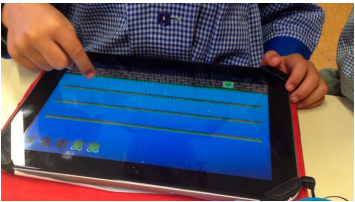
\includegraphics[width=8cm]{figures/sami_interacting.PNG}
    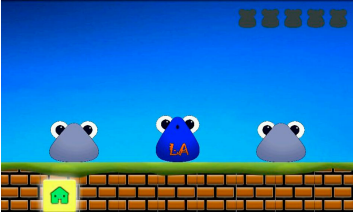
\includegraphics[width=8cm]{figures/sami_memory.PNG}
    \caption{SAMI Application \protect\cite{paule2017music}}
    \label{fig:sami_memory}
    \
\end{figure}

% Having simple layouts can also help ease the use of the application especially for children. According to a feedback for the design of a tool called iBUAT (Paper Prototyping of Interactive Game Design
% Authoring Tool for Children) by \citeA{ibharim2014ibuat}, the children were more attracted to the simple interface that was easy to navigate and understand. Using well designed applications can attract the attention of children \cite{chung2017designing} and can also increase the pace of learning \cite{cohen2011young}. We can use this for Firefly by designing the interface and using icons that are attractive to children. Figure \ref{fig:iBuAT_ui} and \ref{fig:ICON_DES} show examples of interfaces that children are more attracted to.

\begin{figure}[H]
    \centering
    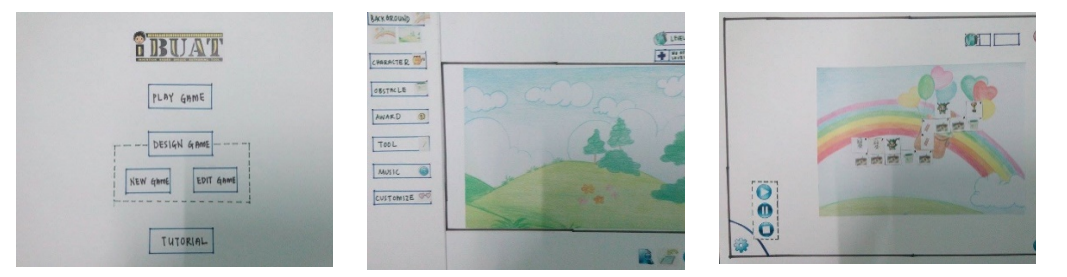
\includegraphics[width=14cm]{figures/iBUAT_design.PNG}
    \caption{iBUAT Interface design \protect\cite{ibharim2014ibuat}}
    \label{fig:iBuAT_ui}
\end{figure}


\begin{figure}[H]
    \centering
    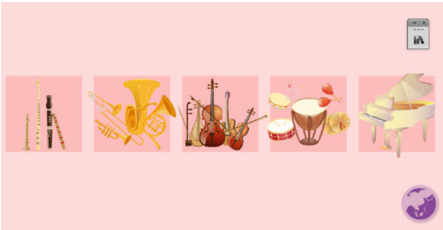
\includegraphics{figures/chung_icons.PNG}
    \caption{Icon Design \protect\cite{chung2017designing}}
    \label{fig:ICON_DES}
\end{figure}

CAI applications have many uses inside and outside school settings, but there are limitations to using it. The results of its effectiveness and quality highly depends on the teaching material and instructional approach \cite{aqda2011comparative}. Making CAI applications must also consider using the student model, which is the acknowledgement of the presence and the limits of the knowledge of the user \cite{self1974student}. This means making multiple levels for difficulties of the CAI application for the user. The sandbox environment or sandbox approach is also another educational tool that lets the users explore the tool and learn how to use it on their own without any instructional procedures like CAI. This allows the application for the users to learn and explore FireflyX for themselves.

%martX
In order for CAI applications to be even developed in the first place, the concept of human factors must be understood. Human factors are defined as a discipline concerned with understanding the interactions among humans and elements of a system in order to be able optimize human well-being when interacting with these systems \cite{salvendy2012handbook}. Experts in the field contribute to the different tasks associated with these systems in order to make these systems have the ability to be compatible with the needs, abilities and limitations of people. 

However, systems not optimized or worse for human interaction are also found to be detrimental to the people using it \cite{foley1984human}. For example a badly designed user interface may lead to negative outcomes. Negative outcomes include lower productivity, increased frustration and the need for redesigning to eliminate these outcomes. Due to this, the need for understanding Human factors arises.

To help maximize the usability of an application, specific human factors related to the application's purpose must be observed. For example, if an application's purpose is to educate, then the factors that should be taken into account are the student's experiences and limitations such as reading capabilities \cite{radu2014augmented}. By knowing the users capabilities, an application can be better used by the users due to it being designed to the users needs or specifications. One specific application of this is scaffolding. Scaffolding is defined as something or someone that provides assistance when a child is acquiring a new skill during the execution of the actual skill itself \cite{strommen1998interface}. However, scaffolding can come in many different forms but finding the most optimal form of scaffolding can be done by understanding the specific user needs and limitations.

Since FireflyX would be assisting in learning music for children, factors in education and children can should be taken into account. A study mentions that these factors include the children's imagination, their media generation and age differences \cite{oosterholt1996interaction}. The importance of imagination comes in involving the children in the concept phase when discussing new products to them. Their generation is important as they wont respond much to things that have nothing to do with their generation. Also their generation usually also makes them have certain skills for using technology compared with other generations. Finally the age differences are important because a child grows fast mentally and physically making them have different views to each other if they are even a few years in age apart.


% \usepackage{color}

% \begin{landscape}
% \begin{table}[]
% \begin{tabular}{|l|l|l|l|}
% \hline
% Authors                                                                                                                                                      & Focus                                                                        & Theory/Principle                                                                      & Contributions/Details                                                                                                                                                                                                                                                                                                                                                                                                         \\ \hline
% \begin{tabular}[c]{@{}l@{}}Aqda, Hamidi, \& Rahimi(2011);\\ Chung, Wu, (2017; Arnold (1997);\\ Barrow, Markman, Rouse (2008);\\ Pennycook(1985)\end{tabular} & \begin{tabular}[c]{@{}l@{}}Computer-aided\\ Instruction\end{tabular}         & \begin{tabular}[c]{@{}l@{}}Advantages and\\ disadvantages\\ of using CAI\end{tabular} & \begin{tabular}[c]{@{}l@{}}CAI gives student a private\\ learning space, assists in \\ teaching in the learning\\ process of children. But \\ Poorly design systems can \\ have big negative effects.\end{tabular}                                                                                                                                                                                                            \\ \hline
% \begin{tabular}[c]{@{}l@{}}Levinowitz (1999);\\ Chung, Wu(2017)\end{tabular}                                                                                 & \begin{tabular}[c]{@{}l@{}}Children Learning\\ using Technology\end{tabular} & Visualization Cues                                                                    & \begin{tabular}[c]{@{}l@{}}We can use visual cues in\\ order to represent music\\ properties for Firefly.\end{tabular}                                                                                                                                                                                                                                                                                                        \\ \hline
% \begin{tabular}[c]{@{}l@{}}Cohen, Hadley, Frank (2011);\\ Chung, Wu (2017)\end{tabular}                                                                      & \begin{tabular}[c]{@{}l@{}}Computer-aided\\ applications\end{tabular}        & Interface Design                                                                      & \begin{tabular}[c]{@{}l@{}}Good interface design and\\ icons can encourage and\\ attract the attention of children\\ to use our application.\end{tabular}                                                                                                                                                                                                                                                                     \\ \hline
% \begin{tabular}[c]{@{}l@{}}Czaja, \& Lee,(2007);\\ qda, Hamidi, \& Rahimi(2011);\\ Self (1974);\\ Aqda, Hamidi, \& Rahimi (2011)\end{tabular}                & \begin{tabular}[c]{@{}l@{}}Computer-aided\\ Instruction\end{tabular}         & \begin{tabular}[c]{@{}l@{}}Importance of\\ Designing CAI\end{tabular}                 & \begin{tabular}[c]{@{}l@{}}The evolution of technology\\ has allowed it to be more accessible\\ and mobile to people. The teaching \\ material and instructional approach \\ greatly affect the quality of education \\ of using computer-aided instruction\\ applications. CAI applications must \\ acknowledge a ”student model”. \\ Difficulty of the instructions depend \\ on the knowledge of the student.\end{tabular} \\ \hline

% \end{tabular}
% \end{table}
% \end{landscape}

% \begin{landscape}
% \begin{table}[]
% \begin{tabular}{|l|l|l|l|}
% \hline
% Authors                                                                       & Focus         & Theory/Principle                                                         & Contributions/Details                                                                                                                                                                                                                                                                                                                                \\ \hline
% Salvendy (2012)                                                               & Human Factors & \begin{tabular}[c]{@{}l@{}}Definition of \\ Human Factors\end{tabular}   & \begin{tabular}[c]{@{}l@{}}Human factors is a discipline that\\ deals with understanding human\\ interaction in order to maximize\\ human well being when designing\\ systems.\end{tabular}                                                                                                                                                          \\ \hline
% Foley, Wallace \& Chan (1984)                                                 & Human Factors & \begin{tabular}[c]{@{}l@{}}Importance of\\ Human Factors\end{tabular}    & \begin{tabular}[c]{@{}l@{}}Systems that do not think about\\ these factors may lead to negative\\ outcomes such as lower productivity\end{tabular}                                                                                                                                                                                                   \\ \hline
% Radu (2014); Stronmen (1998)                                                  & Human Factors & \begin{tabular}[c]{@{}l@{}}Example of Using\\ Human Factors\end{tabular} & \begin{tabular}[c]{@{}l@{}}By researching and understanding \\ the user needs or capabilities, the \\ system can be better used by the\\ users. One application of this is \\ scaffolding. There are many ways to\\ implement scaffolding but  knowing \\ human factors can lead to the best\\ implementation catered to a user\\ need.\end{tabular} \\ \hline
% \begin{tabular}[c]{@{}l@{}}Oosterholt, Kusano \& Vries \\ (1996)\end{tabular} & Human Factors & \begin{tabular}[c]{@{}l@{}}Human Factors of\\ Children\end{tabular}      & \begin{tabular}[c]{@{}l@{}}Children have human factors related \\ to education. These factors include \\ the children's imagination, their \\ media generation and age differences.\end{tabular}                                                                                                                                                     \\ \hline
% \end{tabular}
% \end{table}
% \end{landscape}
\begin{landscape}
\begin{table}[]
\caption{Related Studies on CAI and Human Factors of Children in Learning Music}
\begin{tabular}{|l|l|l|l|}
\hline
Authors                                                                                                                                                                                                                              & Focus                                                                        & Theory/Principle                                                                      & Contributions/Details                                                                                                                                                                                                                                                                                                                                                                                                         \\ \hline
\begin{tabular}[c]{@{}l@{}}Aqda, Hamidi, \& Rahimi(2011);\\ Chung, Wu, (2017; Arnold (1997);\\ Barrow, Markman, Rouse (2008);\\ Pennycook(1985); Cohen, Hadley, \\ \& Frank (2011); Self (1974);\\ Czaja, \& Lee,(2007)\end{tabular} & \begin{tabular}[c]{@{}l@{}}Computer-aided\\ Instruction\end{tabular}         & \begin{tabular}[c]{@{}l@{}}Advantages and\\ disadvantages\\ of using CAI\end{tabular} & \begin{tabular}[c]{@{}l@{}}CAI gives student a private\\ learning space, assists in\\ teaching in the learning\\ process of children. Good designed \\ systems make it more usable for \\ children. Poorly designed systems can \\ have big negative effects. Difficulty \\ of the instructions depend on \\ the knowledge of the student.\end{tabular}                                                                       \\ \hline
\begin{tabular}[c]{@{}l@{}}Levinowitz (1999);\\ Chung, Wu(2017)\end{tabular}                                                                                                                                                         & \begin{tabular}[c]{@{}l@{}}Children Learning\\ using Technology\end{tabular} & Visualization Cues                                                                    & \begin{tabular}[c]{@{}l@{}}We can use visual cues in\\ order to represent music\\ properties for Firefly.\end{tabular}                                                                                                                                                                                                                                                                                                        \\ \hline
\begin{tabular}[c]{@{}l@{}}Salvendy (2012)\\ Foley, Wallace \& Chan (1984)\\ Radu (2014); \\ Stronmen (1998)\end{tabular}                                                                                                            & Human Factors                                                                & \begin{tabular}[c]{@{}l@{}}Definition of\\ Human Factors\end{tabular}                 & \begin{tabular}[c]{@{}l@{}}Human factors is a discipline that\\ deals with understanding human\\ interaction in order to maximize\\ human well being when designing\\ systems. Systems that do not think about\\  these factors may lead to negative\\ outcomes such as lower productivity.\\ By researching and understanding\\ the user needs or capabilities, the\\ system can be better used by the\\ users.\end{tabular} \\ \hline
\begin{tabular}[c]{@{}l@{}}Oosterholt, Kusano \\ \& Vries (1996)\end{tabular}                                                                                                                                                        & Human Factors                                                                & \begin{tabular}[c]{@{}l@{}}Human Factors of\\ Children\end{tabular}     & \begin{tabular}[c]{@{}l@{}}Children have human factors related to \\ education. These factors include\\ the children's imagination, their \\ media generation and age differences\end{tabular}                                                                                                                                                                                                                                \\ \hline
\end{tabular}
\end{table}
\end{landscape}

\section{Sandbox Environment and other Dynamic Interfaces}

This section provides an analysis on how different studies made use of sandbox environments. This will also highlight the results of testing these sandbox environments. It is important that we understand how to properly implement a suitable environment for the children and how to properly conduct testing on them while learning respect to these sandbox environments.

A sandbox environment is an environment, usually set to encourage playfulness, where users can use it as they like. A sandbox environment can be created by implementing the sandbox approach to a software where it is executed it in a specific operating system environment \cite{prevelakis2001sandboxing}. The sandbox approach also encourages users to play boundlessly, thereby increasing their curiosity and engagement in using the environment \cite{goldberg1996secure}.

In the outside world context, children prefer playing games because it stimulates their minds and helps them think creatively \cite{martin1999social, inal2007flow}. The same is also considered in a virtual environment such as an app, children are able to emulate playing outside by using a sandbox environment in an app. The use of apps have been found to increase visual stimulation, improve their navigation skills and be familiarized with music \cite{burton2016music}.

One example of an application that implemented a sandbox approach is Scratch. It allows users to drag and drop blocks to control 2D graphical objects moving on the background, Figure \ref{fig:Scratch_User_Interface} shows a sample of the interface of Scratch. One of the most important feature of Scratch is that it is always live, meaning it requires no compilation step or run mode. Users can also add blocks while a script is running. This lets users be engaged with their projects and always be able to tinker with the blocks \cite{maloney2010scratch}. In the study of \citeA{ouahbi2015learning}, high school students were able grasp programming concepts, and syntax was also not an issue for them. In addition to this, Scratch allows easy visualization of how the algorithm is looks like, and in effect increasing a user’s motivation to learn programming \cite{erol2017effects}. By implementing these features, Scratch is able to provide users a sandbox environment that enables them to learn programming. 

\newpage

\begin{figure}[H]
    \centering
    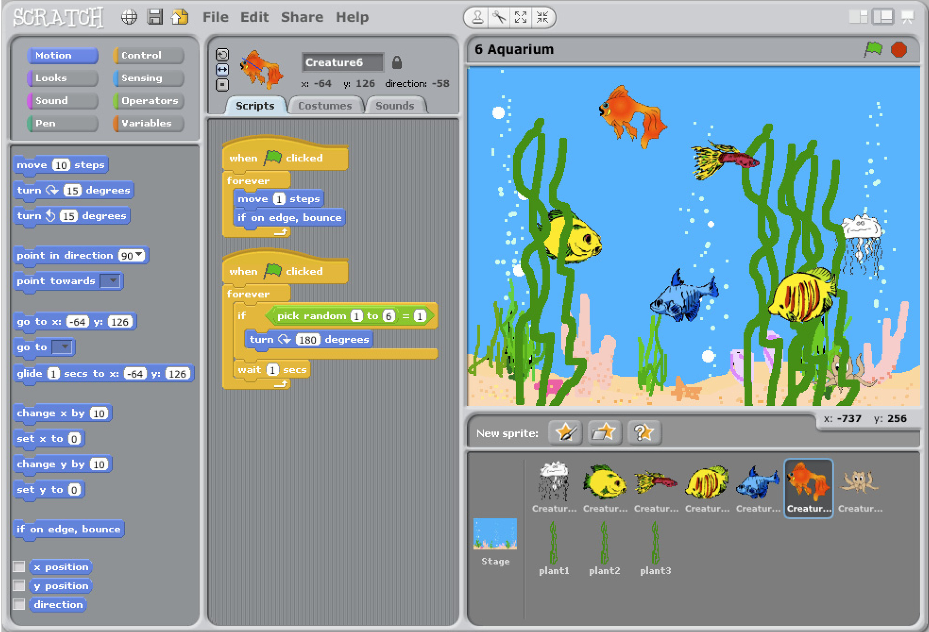
\includegraphics[width=12cm]{figures/Scratch_UI.png}
    \caption{The Scratch User Interface \protect\cite{maloney2010scratch}}
    \label{fig:Scratch_User_Interface}
\end{figure}

Sonification Sandbox was developed in the study of \citeA{walker2003sonification}. It was continued by \citeA{davison2007sonification} and improved on several features and added some new ones as well. It is a graphical toolkit that allows users to map several data sets to timbre, pitch, volume, and pan, with full control over the default, minimum, maximum, and polarity for each attribute. Figure \ref{fig:Sonification_Mappings_Panel} shows a sample interface of the mapping panel and Figure \ref{fig:Sonification_Graph_Panel} shows how the data are graphed. It emulates the sandboxes in playgrounds by making it compatible to all, creating a sandbox that fits all. 

\begin{figure}[H]
    \centering
    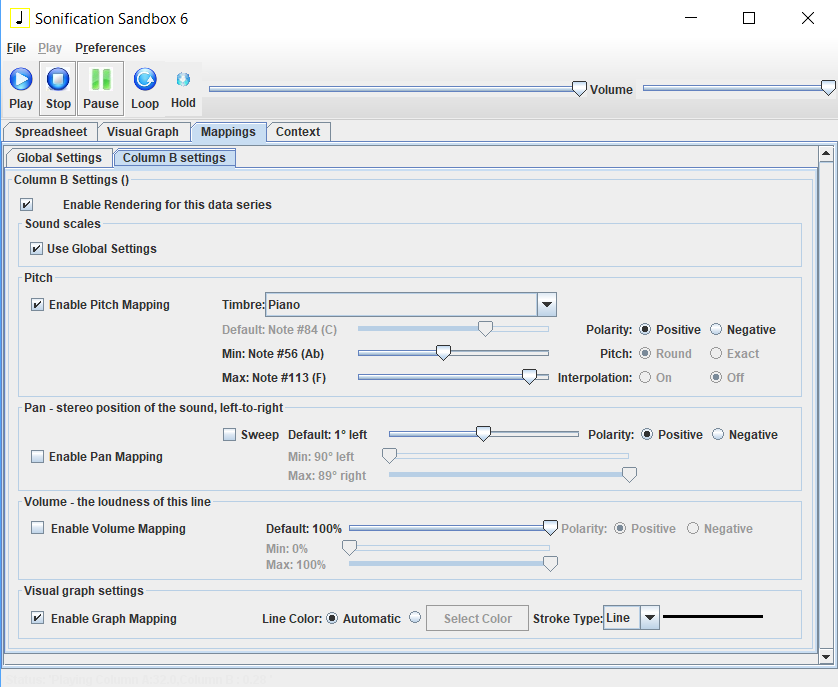
\includegraphics[width=10cm]{figures/Sonification_Mappings_Panel.png}
    \caption{The Mappings Panel for the Sonification Sandbox \protect\cite{walker2003sonification}}
    \label{fig:Sonification_Mappings_Panel}
\end{figure}

\begin{figure}[H]
    \centering
    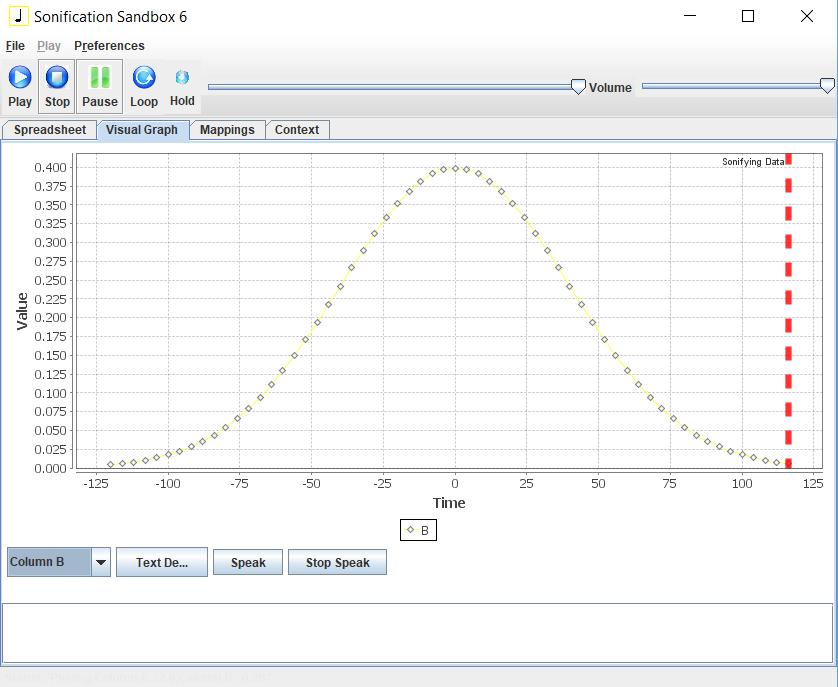
\includegraphics[width=10cm]{figures/Sonification_Graph_Panel.jpg}
    \caption{The Visual Graph Panel for the Sonification Sandbox \protect\cite{walker2003sonification}}
    \label{fig:Sonification_Graph_Panel}
\end{figure}

\newpage

The study of \citeA{paule2017music} developed and evaluated SAMI (Software for music learning in early childhood education). SAMI is a mobile app designed to aid children learning music. The study evaluated SAMI by separating the children into two groups. The control group used Montessori bells, while the experimental group used SAMI. The experimental group was divided into groups of five  and invited to use a tablet in a quiet room outside the classroom with child-sized tables and chairs. The children used SAMI over five sessions divided weekly. Data collection was carried out in four phases. The experiment allotted one session for the children to get familiar with SAMI. The children would have to observe how the mascot moves and sings to each note. The children were then asked questions and when answered correctly the child gets a reward. The second phase observed the children's development of sound discrimination. Phase 3 conducted interviews with the children which was done after three weeks after phase 2. The authors used a semi-structured format asking them which was their favourite game, the one they liked the least and their perception of learning as seen in Figure \ref{fig:children_questionnaire}. In the end, surveys and interviews with children show evidence on the positive effect of technology on children’s motivation and interest for the SAMI group.
% Figure \ref{fig:sami_game1} shows the sample interface of one of the games.
\begin{figure}[H]
    \centering
    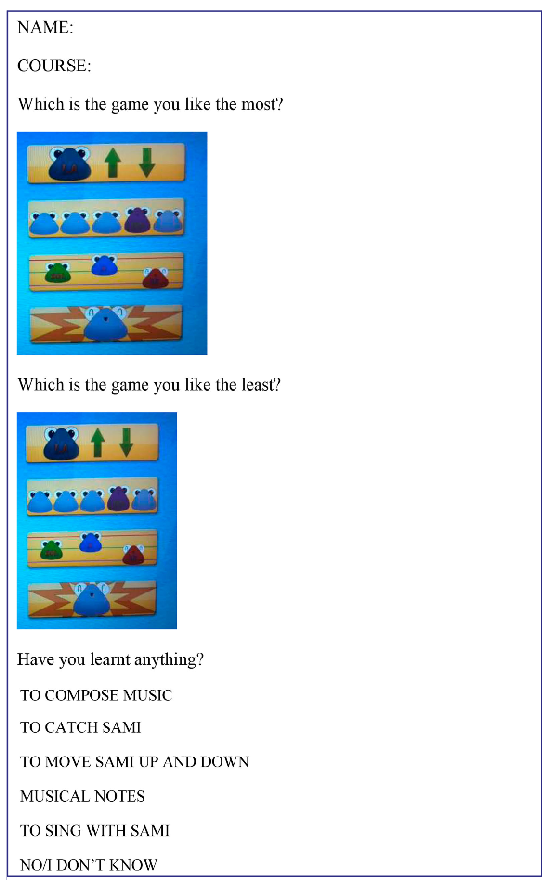
\includegraphics[width=6.5cm]{SAMI_Questionare.png}
    \caption{Children's questionnaire \protect\cite{paule2017music}} 
    \label{fig:children_questionnaire}
\end{figure}
% \begin{figure}[h]
%     \centering
%     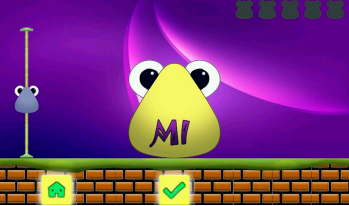
\includegraphics[width=8cm]{sami_game1.PNG}
%     \caption{SAMI Game}
%     \label{fig:sami_game1}
% \end{figure}

\newpage

In the study conducted by \citeA{zhou2011mogclass}, the authors developed and tested MOGCLASS. MOGCLASS is a multimodal collaborative music environment. By using MOGCLASS, teachers are able to manage the classroom better and lets students have a better musical learning environment. In the experiment for MOGCLASS, the music teacher is given a lesson plan which starts with the introduction of the instrument by showing students how to play some notes. Next, the students are asked to answer Q2-Q5 in the questionnaire as seen in table \ref{fig:mogclass_questionnaire}. Afterwards, The student are taught how to play a simple song where the students can make use scaffolding feature. The scaffolding is used to guide people through the usage of devices with the use of visual hints similar to karaoke. After Learning a simple song they are taught an advanced song. Here, the students can still use the scaffolding. The students are then asked to answer Q1 - Q7 of the questionnaire (table \ref{fig:mogclass_questionnaire}). In the final lesson, students are asked to try to perform the advanced song on their own without the use of the scaffolding. After this lesson, the teacher will grade and assess the students in terms of creativity, style and technical proficiency. Lastly, the students are asked to answer the questionnaire once more.

\begin{table}[H]
    \centering
    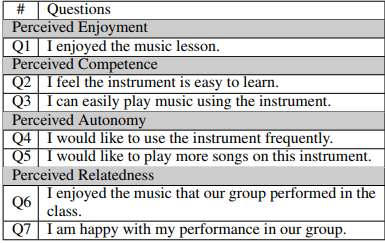
\includegraphics[width=7cm]{mogclass_questionaire.PNG}
    \caption{MOGCLASS Questionnaire \protect\cite{zhou2011mogclass}}
    \label{fig:mogclass_questionnaire}
\end{table}

Xylotism is an interactive game implemented in a sandbox environment that aims to help children learn and teach music to children \cite{elahi2017xylotism}. The study tried to mirror the scenario introduced in the study of \citeA{taheri2016social} where the children trying to learn music is accompanied by a robot and xylophone \cite{taheri2016social}. At the beginning of testing Xylotism, the game's instructions are first described to the child. Then, half of the children were tasked to use the app, while the other half were tasked to use a real xylophone that resembles the app. After 8-12 minutes of playing, the children using the app then switched to using the xylophone, and vice versa. After these, a scenario performed previously by Nima robot \cite{taheri2016social} is simulated, where the instructor plays a rhythm and the child tries his/her best to imitate the instructor. The instructor encourages or warns about the right or wrong answers, respectively. They then used Stambak’s Rhythmic Structures Reproduction test, a test containing 21 easy to hard rhythmic tasks that will assess the participant by having him/her reproduce after hearing \cite{gardner1971children}, in order to gauge how much the child learned.

\label{tab:relBox}
\begin{landscape}
\begin{table}[ht]
\centering
\small
\caption{Related Studies on Sandbox Environments and other Dynamic Interfaces}
\begin{tabular}{|l|l|l|l|} 
\hline
Authors                                                                                                             & Focus                                                                          & Theory/Principle                                                                                                       & Contributions/Details                                                                                                                                                                                                                                                                     \\ 
\hline
\begin{tabular}[c]{@{}l@{}}Prevelakis \& Spinellis (2001);\\Goldberg et al. (1996)\end{tabular}                     & Sandbox Environment                                                            & \begin{tabular}[c]{@{}l@{}}Sandbox environments\\allow users to interact\\with it boundlessly.\end{tabular}            & \begin{tabular}[c]{@{}l@{}}A sandbox approach is \\implemented by executing \\a software in a specific operating\\system environment. This allows\\users to interact with it boundlessly.\end{tabular}                                                                                    \\ 
\hline
\begin{tabular}[c]{@{}l@{}}Marting et al. (1999);\\Inal \& Cagiltay (2007);\\Burton \& Pearsall (2016)\end{tabular} & Children's use of sandboxes                                                    & \begin{tabular}[c]{@{}l@{}}Children prefer playing\\games, in the outside\\world.\end{tabular}                         & \begin{tabular}[c]{@{}l@{}}Children playing games helps them\\think creatively. Being able to play\\without worry stimulates their minds.\\Using apps allow them to emulate this.\end{tabular}                                                                                            \\ 
\hline
\begin{tabular}[c]{@{}l@{}}Walker, Cothran (2003);\\Davidson \& Walker (2007)\end{tabular}                          & \begin{tabular}[c]{@{}l@{}}Sonification in \\sandbox environment \end{tabular} & Sonification                                                                                                           & \begin{tabular}[c]{@{}l@{}}Sonification Sandbox is able to map \\several data sets to timbre, pitch, \\volume, and pan, with full control over\\ each attribute.\end{tabular}                                                         \\ 
\hline
\begin{tabular}[c]{@{}l@{}}Maloney et al. (2010);\\Ouahbi et al. (2015);\\Erol \& Kurt (2017)\\\end{tabular}        & \begin{tabular}[c]{@{}l@{}}Scratch and its sandbox\\environment\end{tabular}   & \begin{tabular}[c]{@{}l@{}}Benefits of Sandbox \\approach\end{tabular}                                                 & \begin{tabular}[c]{@{}l@{}}Scratch is able to help novice learners\\learn programming concepts with\\the use of a sandbox environment.\end{tabular}                                                                                                                                       \\ 
\hline
Paule-Ruiz et al. (2017)                                                                                            & Testing SAMI to children                                                       & \begin{tabular}[c]{@{}l@{}}Children should be\\interviewed and surveyed\\during, and after using the\\app\end{tabular} & \begin{tabular}[c]{@{}l@{}}In-depth process on testing a mobile\\app to children.\end{tabular}                                                                                                                                                                                            \\ 
\hline
Zhou et al. (2011)                                                                                                  & \begin{tabular}[c]{@{}l@{}}Testing MOGCLASS to \\children\end{tabular}         & \begin{tabular}[c]{@{}l@{}}Asking children to answer\\questionnaire should be\\step-by-step\end{tabular}               & \begin{tabular}[c]{@{}l@{}}Children are first shown how to play\\some notes. They are then asked\\some of the questions from the questionnaire.\\After being able to perform simple songs,\\they are again asked some questions. The \\children are then asked to\\answer all the questions.\end{tabular}  \\ 
\hline
\begin{tabular}[c]{@{}l@{}}Elahi et al. (2017);\\Taheri et al. (2016);\end{tabular}                                 & Testing Xylotism to children                                                   & \begin{tabular}[c]{@{}l@{}}Children learn better when\\there is an instructor they\\should follow\end{tabular}         & \begin{tabular}[c]{@{}l@{}}Children are first shown how to use the\\app, after which they are asked to imitate\\the rhythm made by their instructor.\\They are then assessed by using 21\\easy to hard rhythmic tasks.\end{tabular}                                                       \\
\hline
\end{tabular}
\end{table}
\end{landscape}

\section{Review of Related Software}
% This section contains a review of software systems that:
%
% IPR acknowledgement: the following list of items are from Ethel Ong's slides on RRL.
%
% \begin{itemize}
%   \item Belongs to a research area similar to yours
%   \item Addresses a need or domain similar to yours
%   \item Is your predecessor
% \end{itemize}
% \subsection{Perfect Piano}
% Perfect Piano is an application that stimulates a piano and is created by Revontulet Soft Inc. It designed for all ages and can teach how to play the piano by putting labels on piano keys in the screen, then showing corresponding sheet music on top of the screen which shows which keys to press when seeing a specific note. It can also practice a person's skill to listen for melodies and rhythms with a waterfall mode in which keys are seen falling from a height and have to pressed when they reach an appropriate height. 
% %http://www.revontuletsoft.com/
% %https://play.google.com/store/apps/details?id=com.gamestar.perfectpiano

% \subsection{Violin}
% Magical Bow is an application that stimulates a violin and is created by Rubycell. This app teaches users by stimulating a violin and  how to play it, controls include sliding the violin bow up and down to change the note played and sliding the bow side wards to play the note. It helps users learn the proper way to make violin notes by showing them what note they are making when using the bow at a certain angle.
% %https://play.google.com/store/apps/details?id=com.rubycell.violin

% \subsection{Kids Music Instruments Sounds}
% Kids Music Instruments Sounds is an application that multiple simple instruments and is created by Kidstatic Apps.  This app is mainly designed for kids with its simplistic design and simple controls. It shows kids what certain sounds certain instruments play when they are tapped at certain parts. The different instruments for the children to experience include the xylophone, saxophone, drums, and more.
% %http://www.kidstatic.net/
% %https://play.google.com/store/apps/details?id=com.kidstatic.kidsmusicinstruments

% \subsection{iBone}
%  The Pocket Trombone is an application that simulates a trombone and is created by Spoonjack and LLC. It is designed for all ages and teaches the trombone with its multiple Controls that include sliding, wiggling and even blowing into the phone to make music. Learning how to play the trombone is shown by a suggestive program that suggests what notes to be played during a song. If further help is needed, an AI can show the user what the entire song sounds like when the right notes are pressed so they may know if what they are doing is right.
% %http://ibone.spoonjack.com/
% %https://play.google.com/store/apps/details?id=com.spoonjack.ibone&hl=en

There are several music applications that are not sandbox in approach but still provide virtual collaborative environments for expression and composition. One example is the work of \cite{zhou2011mogclass} called MOGCLASS. MOGCLASS is a multimodal collaborative music environment that enhances students’ musical experience and improves teacher’s management of the classroom. This application features an interface for the teacher and a separate interface for the students. The teacher’s interface has features that allow the teacher to manage the class better, while the student’s interface has features that mimic instruments this supports a music technique called scaffolding.

MOGCLASS simulates 3 instruments for the students and can be seen in 3 different student interfaces. The first instrument is called a hitter and it stimulates a drum. It uses an accelerometer in which makes the device detects handshakes and makes a sound proportional to the level of shaking. The second instrument is called a tapper which stimulates a piano. Figure \ref{fig:mogclass_student_interface} also shows how the scaffolding looks like as it is a set of bars that drop down from the top of the screen. The location of the bar shows which note to be played and the size of the bar shows how long the note should be played. The last instrument is the slider and it stimulates a violin. The vertical position of the finger plays different notes on the slider. Figure \ref{fig:mogclass_student_interface} shows the sample student interface of the second instrument which represents the piano.

\begin{figure}[H]
    \centering
    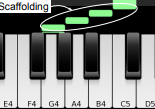
\includegraphics[width=8cm ]{mogclass_studen_interfaces.PNG}
    \caption{MOGCLASS Student Interface \protect\cite{zhou2011mogclass}}
    \label{fig:mogclass_student_interface}
\end{figure}

As for the teacher’s interface which is shown in figure \ref{fig:mogclass_teacher_interface}, it comes with many features that can help manage the class. The teacher can control which instrument the student’s interface will display and which notes it can start with. The teacher can also control if the student is muted or not. Finally, the teacher can choose which song will be used when scaffolding is used in the student’s interface.

\begin{figure}[H]
    \centering
    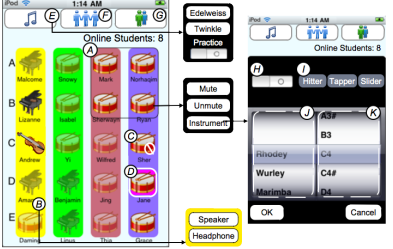
\includegraphics[width=8cm ]{mogclass_teacher_interace.PNG}
    \caption{MOGCLASS Teacher Interface \protect\cite{zhou2011mogclass}}
    \label{fig:mogclass_teacher_interface}
\end{figure}

%The experiment to test out MOGCLASS adopts a between-subjects design which is a experiment where there are multiple groups in which each group is tested in a different way to compare results. The independent variable was the musical instrument. One class was taught with MOGCLASS and the other class was taught with recorders while all other variables were kept constant such as the teacher and the lesson plan. For the duration of the lesson, parts of the questionnaire will be filled up afterwards. 

%The lesson plan of the music teacher starts with introduction of the instrument by teaching how to play the some of the notes (Allow students to answer Questionnaire Q2 - Q5). Afterwards, The student are taught how to play a simple song in which the MOGCLASS students can use scaffolding. Scaffolding is used to guide people through the usage of devices with the use of visual hints similar to karaoke. After Learning a simple song they are taught an advanced song and here the MOGCLASS students can still use the scaffolding (Allow students to answer Questionnaire Q1 – Q7). In the final lesson, students are to try to perform the advanced song on their own and the MOGCLASS students cannot use scaffolding. After this lesson, the teacher will grade and assess the students in terms of creativity, style and technical proficiency and the students will fill up the questionnaire once more (Allow students to answer Questionnaire q1-q1).

%The questionnaire as seen in Figure \ref{fig:mogclass_questionnaire} is divided into 4 parts, enjoyment, competence, autonomy, and relatedness. Each question was rated on a 7- point Likert scale. Results from the experiment and the questionnaires showed that MOGCLASS achieves what is was made for which is effective in motivating students to learn music, improving the way they collaborate with other students as well as helping teachers manage the classroom.

From this application, FireflyX can make use of the scaffolding feature in order to help guide children in learning musical elements. Having a separate teacher and student interface may also be taken into consideration since teachers may help accelerate the learning of the children as well. 

%MOGCLASS
% https://sci-hub.tw/https://dl.acm.org/citation.cfm?id=1979016&fbclid=IwAR03o9hxpQ1LsxIX_NsdQ7fQtPRK31aKool3jAPYeUDz3TIxAz8chPiXrcc

Aside from MOGCLASS, More scaffolding can be found in a study by \citeA{jorgensen2015mobile}. This includes virtual instruments for children so that they may engage more in museum setups. The application has three instruments to use being the harpsichord, double bass and the viola. The application suggests using them one by one and in the end all past performances are played back simultaneously revealing that playing instruments together make a composition. All the instruments have colored rectangles that scroll downwards which depicts the note they should be playing. These rectangles are a form of scaffolding.

For the harpsichord, the colored rectangles are above a keyboard and the rectangles determine which key should be pressed for the correct note to be played. For the double bass, there are colored strings below and the colored rectangles refer to which string has to be plucked in order to play the correct note. The viola, is similar to the double bass but instead of plucking, children have to swipe on the correct string in order to stimulate using a bow and to play the correct note. FireflyX might be able to use the different forms of scaffolding presented here. We can also make use of the way this application simultaneously plays different instruments at once for when there are multiple fireflies created.

%  responses may serve as a way to guide the users if they are doing correct or not. Firefly may be able to use the feedback system given my Nima to motivate children further in their usage of Firefly.\begin{figure}[Theseh]
%     \centering
%     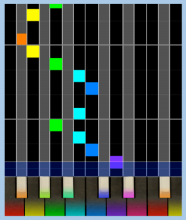
\includegraphics[width=8cm \textwidth]{museum_harpsichord.PNG}
%     \caption{Music Authoring Application \protect\cite{jorgensen2015mobile}}
%     \label{fig:museumHarpsichord}
% \end{figure}

% \begin{figure}[h]
%     \centering
%     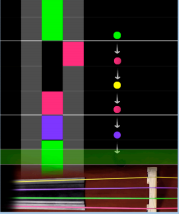
\includegraphics[width=1 \textwidth]{museum_double_bass.PNG}
%     \caption{Music Authoring Application \protect\cite{jorgensen2015mobile}}
%     \label{fig:museumBass}
% \end{figure}

% \begin{figure}[ht]
%     \centering
%     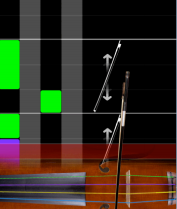
\includegraphics[width=8cm ]{museum_viola.PNG}
%     \caption{Viola Interface \protect\cite{jorgensen2015mobile}}
%     \label{fig:museumViola}
% \end{figure}

% A Mobile Music Museum Experience for Children
% https://nime2015.lsu.edu/proceedings/267/0267-paper.pdf

The development of musical tools have migrated to mobile environments as well. One study is SAMI by \cite{paule2017music}. SAMI is a music learning application for children using tablet-computers. For it to be able to teach music, it has 4 games that are designed to facilitate learning and encourage children's thinking and creativity. SAMI, a triangular blob with large eyes, is also the mascot of the game and is interacted with in all of the games. The first game aims to educate the children by using the ears to identify several sounds. In short, the first game is a memory game using notes. The game plays a note and the task of the user is to tap SAMI with a similar noise representing that note. Each SAMI has a color at first to determine the note. The second game is a memory game with order of the notes wherein the children have to tap on SAMIs in the correct order. This aims to teach notes as if they were part of a major chord. The third game is a reactive tapping game and aims to teach fine motor skills required to play instruments. There are 3 rows and each location of SAMI places a different note. SAMIs appear and the child needs to tap on SAMI before they disappear. SAMIs on the top row play higher pitched notes when tapped. The last game is a composing game which combines all the previous games and has the child try to compose with SAMIs by having arrange SAMI’s in different heights and at a certain arrangement. These games may serve as an inspiration on how some features or parts of FireflyX may be able to be implemented.


% Music learning in preschool with mobile devices (SAMI)
% https://sci-hub.tw/https://doi.org/10.1080/0144929X.2016.1198421


Just as SAMI teaches with its games, an application by \citeA{elahi2017xylotism} also teaches with instructions. This application features a bot named Nima that gives instructions. The instructions given by Nima follow a step by step process. The initial stages would be instructions to get the user to understand notes. These instructions include commands for the user to do something or questions to ask the user. The later stages would involve trying to make the user replicate rhythms. 

Based on the user's actions, Nima also gives some feedback to help guide the user. When the user is doing well, Nima can respond by doing dances and saying things like that's great, bravo, etc. If the user makes a mistake, Nima says things like pay attention or try again. Aside from these responses, there are also emojis showing happy faces or sad faces depending on the user's actions as well. From this application, FireflyX may be able to use the instructions and feedback system given by Nima. The instruction system may help guide the children on the usage of FireflyX. The feedback system may encourage the children with their usage of FireflyX.

%Xylotism
%https://sci-hub.tw/https://link.springer.com/chapter/10.1007/978-3-319-70022-9_72


Aside from Xylotism, there are other musical applications where children’s preferences are considered especially in measuring engagement or fun. One study is by \citeA{burton2016music}. Common application preferences by children include easy to navigate menus, a variety of ways to engage, visual stimulation, familiar musical material, music that continues without manipulation, and animated characters such as animals, babies, children, movement, and/or dancing.

A table in the study as seen in Table \ref{fig:child_checklist} shows different applications wherein the applications in bold are considered the child friendly applications while the italicized ones aren’t. The table also shows if the application has features that children like. The less child friendly apps are similar to the child friendly app above it in regards on what it aims to teach. 


\begin{table}
\centering
\caption{Child Friendly Features Checklist \protect\cite{burton2016music}}
\label{fig:child_checklist}
\scalebox{0.8}{\begin{tabular}{|l|l|l|l|l|l|l|} 
\hline
Application                   & Characters                            & Movement                              & Dancing                               & Animation                             & Children                              & Songs                                  \\ 
\hline
\textbf{Juno's Piano}         &                                       & \textcolor[rgb]{0.133,0.133,0.133}{\checkmark} & \textcolor[rgb]{0.133,0.133,0.133}{\checkmark} & \textcolor[rgb]{0.133,0.133,0.133}{\checkmark} &                                       &                                        \\ 
\hline
\textit{Virtuoso Piano}       &                                       &                                       &                                       &                                       &                                       &                                        \\ 
\hline
\textbf{Monkey Drum}          & \textcolor[rgb]{0.133,0.133,0.133}{\checkmark} & \textcolor[rgb]{0.133,0.133,0.133}{\checkmark} & \textcolor[rgb]{0.133,0.133,0.133}{\checkmark} & \textcolor[rgb]{0.133,0.133,0.133}{\checkmark} &                                       &                                        \\ 
\hline
\textit{Percussive}           &                                       &                                       &                                       &                                       &                                       &                                        \\ 
\hline
\textbf{Toca Band}            & \textcolor[rgb]{0.133,0.133,0.133}{\checkmark} & \textcolor[rgb]{0.133,0.133,0.133}{\checkmark} & \textcolor[rgb]{0.133,0.133,0.133}{\checkmark} & \textcolor[rgb]{0.133,0.133,0.133}{\checkmark} & \textcolor[rgb]{0.133,0.133,0.133}{\checkmark} &                                        \\ 
\hline
\textit{Loopseque}            &                                       &                                       &                                       & \textcolor[rgb]{0.133,0.133,0.133}{\checkmark} &                                       &                                        \\ 
\hline
\textbf{Ambient Mood}         & \textcolor[rgb]{0.133,0.133,0.133}{\checkmark} & \textcolor[rgb]{0.133,0.133,0.133}{\checkmark} &                                       & \textcolor[rgb]{0.133,0.133,0.133}{\checkmark} &                                       &                                        \\ 
\hline
\textit{Bloom HD}             &                                       &                                       &                                       &                                       &                                       &                                        \\ 
\hline
\textbf{Kids Song Collection} & \textcolor[rgb]{0.133,0.133,0.133}{\checkmark} & \textcolor[rgb]{0.133,0.133,0.133}{\checkmark} &                                       & \textcolor[rgb]{0.133,0.133,0.133}{\checkmark} & \textcolor[rgb]{0.133,0.133,0.133}{\checkmark} & \textcolor[rgb]{0.133,0.133,0.133}{\checkmark}  \\ 
\hline
\textit{iTunes Collection}    &                                       &                                       &                                       &                                       & \textcolor[rgb]{0.133,0.133,0.133}{\checkmark} & \textcolor[rgb]{0.133,0.133,0.133}{\checkmark}  \\ 
\hline
\textbf{Lily Rock Band}       & \textcolor[rgb]{0.133,0.133,0.133}{\checkmark} & \textcolor[rgb]{0.133,0.133,0.133}{\checkmark} & \textcolor[rgb]{0.133,0.133,0.133}{\checkmark} & \textcolor[rgb]{0.133,0.133,0.133}{\checkmark} & \textcolor[rgb]{0.133,0.133,0.133}{\checkmark} & \textcolor[rgb]{0.133,0.133,0.133}{\checkmark}  \\ 
\hline
\textit{Rockmate}             &                                       &                                       &                                       &                                       &                                       &                                        \\
\hline
\end{tabular}}

\end{table}

The first two apps for example aim to teach melody according to the study. The first application, Juno’s Piano is treated by the study as the child friendly application due to it having the features normally preferred by children as seen in the table. In Figure \ref{fig:iPad_friendly}, the application has bright colors and a cute character on top of the piano. 

\begin{figure}[H]
    \centering
    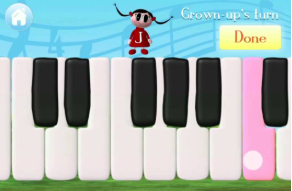
\includegraphics[width=10cm]{ipad_kid_friendy.PNG}
    \caption{iPad Kid Friendly Example \protect\cite{burton2016music}}
    \label{fig:iPad_friendly}
\end{figure}

However, Virtuoso Piano is missing these preferences thus making the study treat it as the less child friendly application. In figure \ref{fig:iPad_unfriendly}, the application is missing characters and only has some dull colors to it. 

\begin{figure}[H]
    \centering
    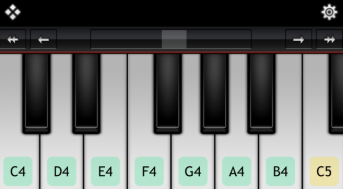
\includegraphics[width=8cm]{ipad_not_kid_friendly.PNG}
    \caption{iPad Not Kid Friendly Example \protect\cite{burton2016music}}
    \label{fig:iPad_unfriendly}
\end{figure}

In order for children to use FireflyX longer, FireflyX will use some features, which will be tested through the different iterations, that children find appealing as seen from the child friendly applications and try to avoid missing some features such as the less child friendly applications.

%ipad prefences
% https://sci-hub.tw/https://doi.org/10.1177/1321103X16642630

Not all applications may be usable for all children however. Some children such as the one’s diagnosed with autism spectrum disorders may be in need of social skills so that they may be able to live independently when they reach adulthood. A study by \citeA{hourcade2012multitouch}, includes the creation of applications in order to promote social skills to these children. One of the applications created was a music authoring application. 

The application has a harp like screen and the children are able to choose tiles which determine what note they would play, the notes on the higher part of the screen depicting higher notes and vice versa. The notes are played in sequence, with the note that is currently played turning green. Since this application aims to promote social skills as well, the music authoring app was designed to be used by multiple children. The multi-touch feature where it can have multiple notes selected at once makes it possible for children to edit at once. 

Since the study also shows that the children mentioned using the application makes it more enjoyable. FireflyX may be able to incorporate the collaborative multi touch feature this application presents as it may attend to more than one children at once so that FireflyX maybe more enjoyable for children.
%This application would be used for collaborative music creation in which children are asked to put a few notes before passing the tablet to another kid. This is for the children to appreciate social interaction. Feedback from the children related to the application is that the music authoring was the best part among the multiple applications and they liked the song they made with their friends. However they also commented that they wanted more instruments. It is found out that technology may be enough of an incentive to improve the quality of social interactions.

% \begin{figure}[!htb]
%     \centering
%     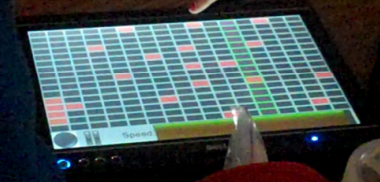
\includegraphics[width=13cm]{music_authoring.PNG}
%     \caption{Music Authoring Application \protect\cite{hourcade2012multitouch}}
%     \label{fig:musicAuthoring}
% \end{figure}


% Multitouch tablet applications and activities to enhance the social
% skills of children with autism spectrum disorders
% https://sci-hub.tw/https://dl.acm.org/citation.cfm?id=2125154


% Mart's Synthesis Table
\begin{landscape}
\begin{table}
\centering
\caption{Related Systems for Children Music Learning Tools}
\begin{tabular}{|l|l|l|l|} 
\hline
Authors                                                                                                                                                                                      & Name of System                                                                         & Platform                                                                            & Comments/Findings                                                                                                                                                                                                     \\ 
\hline
\begin{tabular}[c]{@{}l@{}}Percival et al. (2011);\\ Jorgensen et al. (2015)\end{tabular}                                                                     & \begin{tabular}[c]{@{}l@{}}MOGCLASS;\\ A Mobile Music \\Museum \\Experience \\for Children\end{tabular}           & \begin{tabular}[c]{@{}l@{}}Ipod Touch; \\ Tablet\end{tabular}                         & \begin{tabular}[c]{@{}l@{}}Both show basic scaffolding for various\\ instruments.The first system features \\a separate teacher and student interface. \\The second combines music played and \\plays it back to the user.\end{tabular}                         \\ 
\hline
\begin{tabular}[c]{@{}l@{}} Burton \& Pearsall (2016)\\\end{tabular}                                                      & \begin{tabular}[c]{@{}l@{}}NA \end{tabular}         & \begin{tabular}[c]{@{}l@{}}Ipad \end{tabular}                       & \begin{tabular}[c]{@{}l@{}}It differentiates popular kid-friendly \\applications and less kid-friendly \\applications using common preferences\\ by kids in applications. \end{tabular}  \\ 
\hline
\begin{tabular}[c]{@{}l@{}}{\'A}lvarez-Garc{\'\i}a et al. (2016);\\ Ahmadi et al. (2017) \end{tabular}                                                           & \begin{tabular}[c]{@{}l@{}}SAMI;\\ Xylotism \end{tabular} & Tablet                                                                        & \begin{tabular}[c]{@{}l@{}}Both systems have integrated learning \\music in a step by step process by using \\games. They both use child friendly graphics \\and motivation for the child as they \\learn musical concepts. \end{tabular}                                                                                                   \\ 
\hline
\begin{tabular}[c]{@{}l@{}}Bullock-Rest, Hansen,  \& \\Hourcade(2011)\\ \end{tabular} & \begin{tabular}[c]{@{}l@{}}Music Authoring \\ Application \end{tabular}        & Tablet                                                                           & \begin{tabular}[c]{@{}l@{}}Focusses on an application made for social \\interaction. The application aims for children \\to make music together on a harp like screen. \end{tabular}                                                                        \\ 
% \hline                                                \\
\hline
\end{tabular}
\end{table}
\end{landscape}               %-- includes LaTeX source file for Chapter 2: Review of Related Literature
                                  %-- your job: **EDIT THIS FILE** to indicate your review of related literature 

%%%%%%%%%%%%%%%%%%%%%%%%%%%%%%%%%%%%%%%%%%%%%%%%%%%%%%%%%%%%%%%%%%%%%%%%%%%%%%%%%%%%%%%%%%%%%%%%%%%%%%
%
%   Filename    : chapter_3.tex 
%
%   Description : This file will contain your Theoretical Framework.
%                 
%%%%%%%%%%%%%%%%%%%%%%%%%%%%%%%%%%%%%%%%%%%%%%%%%%%%%%%%%%%%%%%%%%%%%%%%%%%%%%%%%%%%%%%%%%%%%%%%%%%%%%

% Please refer to the following resources regarding Theoretical Framework: 

% \begin{itemize}

% \item \url{https://link.springer.com/chapter/10.1007/978-1-4419-1454-5_12}
% \item \url{https://link.springer.com/article/10.1007/s10972-015-9443-2}



% \end{itemize}



\chapter{Theoretical Framework}

This chapter provides a clear discussion of different studies and theories
behind each concept of the study. 
The first section will discuss the theories on Human-Computer Interaction, Interaction Design and also Evaluation methods on User Experience, while the last section will focus on Musical Representation. These will be accompanied on the other hand with theories on how children go about in these respective ideas.

\section{Interaction Design} 
Interaction design as described by \citeA{PreeceRogersSharp15} is \say{designing interactive products to support people in their everyday and working lives}, that helps in creating a user experience that enables the users in their work and interaction with others. People use interactive objects everyday like phones, machines, etc., but not all of these are easy to use or effortless. Interaction design focuses not only about giving people a product but also how it understands how a particular feature can affect how people work as well as how it can improve their experience \cite{dix2009human,PreeceRogersSharp15}.

The aim of interaction design is to integrate usability in designing the system, that makes a product that is easy, effective, and enjoyable to use for the user \cite{PreeceRogersSharp15}. User satisfaction is of vital importance in interaction design.The further study of interaction design have led to experts creating processes and identify a group of design principles. These principles will serve as a help in creating good interfaces for users \cite{PreeceRogersSharp15}.

The use of interaction design will be integrated in the different iterations of designing the application. This theory will be important in identifying the principles that will serve as our guidelines in designing the interactions in the interface.

%Children interaction design
%
%Despite the young age of the field of interaction design for children, There are some basic principles that have been developed by researchers over the years \cite{hourcade2008interaction}. 

%Visual Design
%The important aspects of visual design for the children are the icons, text and the complexity. For humans in general, Icons must be easy to to recognize that it can be interacted, represent what they do properly and are distinguishable from each other. The only difference for children is the size of these icons must be proper for the children. The text has to have minimized usage unless it is an application to teach reading. Finally, the visual complexity of the applications must follow multi-layer strategies. These are strategies where children are presented with a few actions or icons to interact with at first and are presented with more as they progress. 

%Interaction Styles
%There are three main interaction styles. The first being the usage of direct manipulation. The main ideas that direct manipulation utilize include visibility of objects and actions of interest. The visibility of objects and actions of interest involve making objects have distinct look that shows there are actions that can be done to them.

%The actions for the objects must be rapid, reversible, and incremental. The actions must be rapid because children tend to be less patient than adults. If the children do not get quick feedback from the action they are likely to lose interest. If an action cannot be rapid, children must still have some way of knowing the status of an action (such as progress bars), the children must be still able to interact with application in another way during the other action taking place and the children must have an option to cancel the action. Reversibility, meaning actions can be undone, on the other hand encourages children exploration while making them remain in control. An action of resulting in a loss of child's creation might lead to frustration and the child losing the desire to use the application anymore. Finally the need for an incremental actions, meaning step by step actions, is required so children can do complex tasks. Without these incremental actions, children may find themselves stuck in a task and unable to progress due to solution being to complex leading to frustration. 

%Another interaction style is the menu. Children are almost always presented with a menu since even a set of choices can be considered a menu. The problem with menus however comes when choices are not immediately visible such as drop down menus. It is found out that menus that had to be brought up with a were easy to forget especially for children making it confusing for them.

%The last interaction style is text based interaction. This becomes a problem when children need to type for them to interact with a computer but do not know how to type yet. Similar to lack of the lack of ability to type is the lack of knowledge to spell. A problem would arise if  commands need proper spelling but the child is unable to spell them correctly. These interactions may significantly slow down as the child lacks the ability to do them.
%

\subsection{Human-Computer Interaction}
Human-Computer Interaction or also known as (HCI) studies ways on how many different computer technologies affect human activities \cite{dix2009human} and how it enhances the quality of interaction between humans and the computer \cite{baecker2014readings}. Research in this field has been an integral part in the development of early systems, like the graphical interface of Windows 95 and another is that it has greatly improved the World-Wide Web \cite{myers1998brief}. Both these early systems show how HCI research has greatly improved the usability of their system and how further interface improvements has enabled more research to be done on this field. 

\citeauthor{kaptelinin1996activity} characterized the subject Human-Computer Interaction in three dimensions as seen in figure \ref{fig:three_dimensions}. The first is the interaction between the user and the environment which transcends the user interface, it explains how the interaction with computers help people in achieving their goals. Next is development, and he describes this as the user develops from being a novice to often becoming an expert. Last is the individual/social dimension as he characterized the word \say{user} not only as an individual but also as a group or an organization.

\begin{figure}[H]
    \centering
    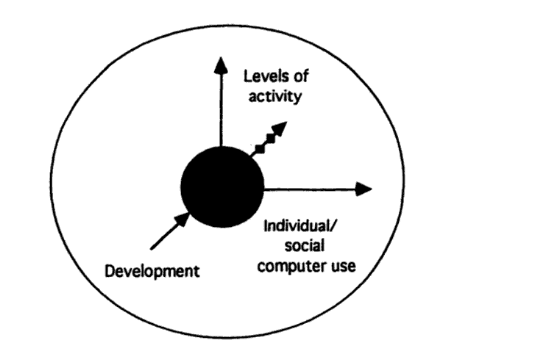
\includegraphics[width=12cm ]{figures/three-dimensions.PNG}
    \caption{HCI Three-Dimensions \protect\cite{kaptelinin1996activity}}
    \label{fig:three_dimensions}
\end{figure}

According to \citeA{inbook}, one of the core topics of studying HCI is the usability of these technologies. Usability according to \citeA{frokjaer2000measuring} is described as taking into three different aspects such as satisfaction, efficiency, and effectiveness. Satisfaction takes into account the use of the system and how comfortable they are with it \citeA{frokjaer2000measuring}. Also described by \citeA{frokjaer2000measuring}, user satisfaction is described as the preferences of the user on the usage of the application on the tasks given to them. Efficiency talks about the relation between users completing the tasks and the resources used to do it \cite{frokjaer2000measuring}. Lastly, effectiveness shows how users properly do their tasks and also achieve certain goals in using the system as determined by some indicators of efficiency for example the completion time of tasks and learning time \cite{frokjaer2000measuring}.

The increase of research in this field as well as the emergence of better technologies has led to the creation of new topics under Human-Computer Interaction like studies on interaction design and user experience.

\subsection{Mobile Interaction Design} 
Interaction Design can also be applied to mobile applications like smartphones and tablets. The change of integrating an application to a mobile platform presents unique challenges in making the interaction. According to \citeA{tidwell2010designing}, these challenges can be summarized into 5 categories. (see Table \ref{Challenges}).

\begin{table}[H]
\centering
\caption{Challenges of Mobile Design} \vspace{0.25em}
\begin{tabular}{|l|l|} 
\hline
\textbf{Challenge}                                                         & \textbf{Description}  \\ 
\hline
Tiny Screen Sizes                                                          & \begin{tabular}[c]{@{}l@{}}In mobile devices space for information is limited. Unlike \\in computers where there are long header menus, in desi-\\igning a mobile application all the excess~assets should be \\removed \cite{tidwell2010designing}.~ ~ ~~\end{tabular}  \\ 
\hline
\begin{tabular}[c]{@{}l@{}}Variable Screen~\\Widths\end{tabular}           & \begin{tabular}[c]{@{}l@{}}The second challenge presents the difficulty in making a~\\design that would scale well on different screen sizes ~\\ \cite{tidwell2010designing}.\end{tabular}                                                                                   \\ 
\hline
Difficultly of Typing                                                      & \begin{tabular}[c]{@{}l@{}}Users do not like it when there is a need to type large am-\\ounts of ext with the keypad \cite{tidwell2010designing}.\end{tabular}                                                                                                           \\ 
\hline
\begin{tabular}[c]{@{}l@{}}Challenging Physical\\Environments\end{tabular} & \begin{tabular}[c]{@{}l@{}}Lastly, people use their mobile devices in different places.\\Places where it could be really bright or dark, during tran-\\sportation, in bed, etc.\cite{tidwell2010designing}.\end{tabular}  \\
\hline
\end{tabular}
\label{Challenges}
\end{table}

For our application the other problems are not to be tackled as much, as firstly the problem on variable screen widths is as not a problem since we will only focus the iPad. Second, the difficultly of typing is not much of a problem since the user will not type a huge amount of text. Third, the environment where the child will use this is not a problem since the place will mostly be indoors. For the application, we will mainly focus on the problems of tiny screen sizes and touch screens seen in Table \ref{Challenges}. The problem of tiny screen sizes in our application is that the size of the iPad screen would be limited as we would also have to properly put the assets on the screen to minimize this. Lastly, the problem on touch screens is what this study aims to solve as we would use gestures aimed to help the interaction between the interface and the user's fingers.

\subsection{Design Principles}
These principles are used in solving the challenges provided in designing the interaction for the users. \citeA{blair2008user} described design principles as \say{clear rules of thumb} that also consist of defined features, \citeA{kimball2013visual} also described that these principles are heuristic methods that help in making decisions. \citeA{norman1999affordance} also states that a successful design comes with a set of underlying principles.  

In making systems developers and companies often think that they should only focus on enhancing the aesthetic appearance of their product in itself rather than also putting equal importance with the overall experience and usability of them \cite{norman1999affordance,blasing2010android,stephanidis2012encyclopedia}. Having a clear idea of the goal of the software from the start is very important, as the interface can be made to achieve the goal that was set and the design should highlight what the goal is \cite{blair2008user}. The overall goal is to design a product that is pleasing to the user for both viewing and using.

\citeA{williams2015non} and \citeA{stephanidis2012encyclopedia} both state four key principles to acknowledge in designing interfaces for different kinds of platforms. The first is \textit{contrast}, this makes the use of shapes, colors, and sizes to draw the users attention. Following this makes it easy for the users to distinguish where they need to focus on. Second, is \textit{repetition}, it talks about having a consistent visual scheme that it makes it easier for the users to recognize. The use of same text, colors, and fonts helps in unifying the design. The third is \textit{alignment}, and this principle talks about the placement of the design elements through out each screen in the system. This principle brings order to each screen and makes the design much more uniform to one another. Last is \textit{proximity}, this principle brings related design elements to be grouped together to show how each element is connected and helps in focusing the users attention. 

Other important principles on the other hand are suggested by \citeA{blair2008user}, one of them is the principle of an Obvious Starting point. This principle can also be used because the user needs to know how to start interacting with the system. The starting point can serve as the point where the user learns more about the interface from the first encounter and cognitively finding patterns helps in the learning. Another is a Clear Reverse and this principle explains how the user can obviously see the way to reverse a particular action or exit the session. Knowing a way to reverse an action or having a clear exit route may give users a sense of confidence in using the system as they need to experience that they can experiment with the system without damaging it.

%Mobile Design Principles
Mobile interfaces have there own limitations when compared to the normal setting of desktop interfaces \cite{gong2004guidelines}. Due to these limitations design principles that are used for desktop interfaces have been modified to aid in creation of mobile interfaces \cite{gong2004guidelines}. \citeA{nilsson2009design} suggests guidelines that help in answering some common issues in mobile interfaces found in Table \ref{Challenges}.

For the problem of screen space an issue identified was the issue of horizontal scrolling this is due to the fact that information on the screen is usually more connected to ones in the same line rather than the ones in different lines \cite{nilsson2009design}. The principle provided to answer this issue is for the attributes on the screen is to be optimized in terms of size and sequence. Changing the layout can help in avoiding the need of horizontal scrolling, an example is changing the screen orientation if the user is given an option to change between landscape and portrait or only given one of the two \cite{nilsson2009design}. Another problem is in typing text, as the keyboard that is provided is usually small for the users that it is hard for the fingers to enter \cite{nilsson2009design}. The principle provided to answer is to provide auto complete of text by trying to predict the word the user is typing by giving suggestions near the current type letters. The last problem is in touch screens, as not all mobile devices are given a stylus that helps with the users interaction with the device. A Principle to help solve this issue is to make the menu choices finger friendly, since the problem lies on the fingers not always hitting the small details of the screen making interaction mechanisms like lists, buttons, menus, etc. finger friendly helps the use in having more control in the application \cite{nilsson2009design}.   

Though the principles presented are not solid rules, nonetheless these principles can still be heavily considered in being followed when designing an interface. The principles mentioned in this subsection will be used as a guide in designing the interface. The four key principles will be taken into consideration in the designing of the assets in the sandbox environment and also in the flow of the usage of the application. We will use the principle of the obvious starting point so that the child will have a screen that they can go back when they are lost. For the clear reverse this is very helpful as the child will make mistakes in using the sandbox and this is helpful so that these mistakes are reversed to let the child finish their tasks. 

\subsection{Gestural Interaction}
The goal of Human Computer Interaction is for humans to naturally interact with technologies like computers for their everyday use \cite{hasan2012human,rautaray2015vision}. For a long time gestures have been considered as a bridge for the humans to interact with these computers, because of the popularity in the usage of hand-held touch screen devices like smart phones and tablets \cite{ruiz2011user,hasan2012human}.

According to a study by \citeA{roth2001gestures}, gestures can be characterized into four. First is \textit{Rest} that actions begin from the point of rest, then it moves away to another position and eventually return to the point of rest. Second characteristic is \textit{Peak or Stroke}, which shows the moment of the gesture which denotes movement. The third is the \textit{Preparation and Recovery Phase}, is when the hand goes back to the resting position. Last is that usually gestures are \textit{Symmetrical}.

There are many user interfaces that gestural interactions have been considered very natural, yet others are harder to understand at first like the multi-touch gestures for devices like tablets compared to other gestures where it can be easily be learned by the user \cite{mortensen_2019}. An example for mobile device users is the simple gesture of swiping left or right compared to a more complex gesture like a multi-finger swipe in a certain direction \cite{mortensen_2019}.

Touch gestures have been seen as an intuitive way of communication between the user and the computer, the actions that build up specific functions makes it natural to use \cite{rautaray2015vision}. In a research done by \citeA{chan2019applying} tasks were made possible with the use of gestures. In integrating the gestures for their mobile musical composition tool they recommended 5 gestures that can be used for similar tasks, these gestures are Tap, Tap & Hold, 1-Finger drag, 2-Finger drag and Pinch. In the different iterations of their research they were able to map the appropriate gestures to accommodate the tasks needed for their composition tool.  

%Children mobile interaction design
%Mobile interaction design gestures.
There are many gestures for mobile applications that use a touch screen. Common gestures include tapping, flicking, sliding, dragging & dropping, rotating, pinching and spreading \cite{aziz2013children}. Generally younger children that are below age 4 may have a hard time with some gestures due to not being familiar with them. Children above age 4 however know how to use all these gestures. Specifically children aged 7-12, have no problem using these gestures to deal with 2D or 3D objects. They do not even have problems doing different gestures in a single application or interface. However they seem to prefer apps that focus on tapping. These children as well prefer more fun and more challenging applications to keep their attention.

For the gestures of the application we will be following the research of \citeA{chan2019applying} as they already provided specific gestures that can be used in a musical application. In the integration of these gestures we would be focusing on how each gesture will help the user in completing their tasks. The specific gestures we would will be focused on the Tap, Tap & Hold and 1-finger drag. For the Tap this gesture will be mostly used in the buttons. The Tap & Hold will be used as a preview of the parts of the firefly model. Lastly the 1-finger drag will be mostly used on assets regarding adjustments and scrolling.

\subsection{Gestalt Principles}
The set of Gestalt Principles comes from psychology, where it says how the human brain will simplify things like elements and recognizing patterns. The Gestalt principles provide six fundamental laws that designers can follow \cite{yee2002user,chapman_2018}.

\begin{enumerate} 
\item Figure/ground
\item Similarity
\item Emergence
\item Closure
\item Continuation
\item Symmetry and Order
\end{enumerate}

\textit{Figure/ground} explains the distinction of the object with relation to the foreground and background of the design.The important thing in this law is how it contrasts and how the object is still visible and understood.

\textit{Similarity} says that humans usually see the same things like size, color, or shape in the design of elements and they tend to group them together. The main use of similarity is to bind elements together that are not necessarily next to each other in the design.

\textit{Emergence} shows how elements that are in range of each other can be grouped together while others also near one another are grouped separately.

\textit{Closure} explains how humans want to see complete objects so if they don't they visually connect missing information through familiarity and patterns seen.

\textit{Continuation} talks about how the human eye will most likely follow a smooth path and it would want to see a clear flow of these visual elements.

\textit{Symmetry and Order} takes into consideration how the design is complete and balanced, because if not time and effort will be exerted by the user in trying to understand it.

The gestalt principles will be used in the application to help design the different parts of the screen. All of these will be taken into consideration but some would be used more, as some assets need these specific principles to be displayed much clearer. In designing the objects in the interface the figure/ground principle helps us in distinguishing these objects from the background so it can be clearly seen by the child. We will use the Similarity principle in designing assets in screen as our target users which are children need to identify visual patterns to be able to complete their tasks. The principle of Emergence will be used in grouping similar assets together to make it easier for the child to identify their functionality. Lastly Symmetry and Order helps us in making the application much more balanced to help the child immediately understand the functionality of the system.

\section{Understanding Children Interaction}
As HCI maybe generally for understanding general humans, we need to focus on children as they have aspects adults do not have. These aspects can result in them having different needs compared to usual adults to where HCI is generally designed for. 

\subsection{CHI Techniques Enabled Through Play}
%CHI PLAY
 CHI Play is a yearly conference that focuses on topics across all areas of play, games and human-computer interaction. They feature papers that show different techniques and practices for games. Some of these are specifically studies are aimed towards children and we can use them for designing our application.

A study by \citeA{gray2018designing} analyzes five commercially available applications for preschool children. They discuss what factors in these applications may lead to children liking or disliking the application. They discuss the importance of characters, support for competence, interaction complexities, and the understanding of buttons and menus. Different game characters with different personalities may increase the chances of a child liking a character which would contribute to the game's enjoyment. Support for competence involves a child getting in-game rewards for doing good in the game. This may increase enjoyment as the children enjoy sharing their achievements however giving the child negative feedback upon doing badly in a game lessens enjoyment as well. Interaction complexities described that confusing tutorials such as one where actual game play cannot be differentiated from a tutorial makes it confusing for the child. This makes them think they were doing things right but it was just the tutorial auto playing for them leading them to perform badly when it came to the actual game. Understanding buttons and menus talk about the difficulty of children have with complex menus and how they ignore text based interaction. They also seem to not understand some symbols and colors of the buttons but can find out what they do with game play. 

A study by \citeA{scheepmaker2018things} discusses that play has a different definition for children as it does for adults. For adults it is generally any enjoyable activity however for children it is something they want to and get to do. Specifically, the children are in control meaning they started playing because they want to. This means they play for them includes things that they do not need to finish or seek approval. An important aspect of play is called appropriation. Playful appropriation is a transformation of situations or elements into fun experiences. An example seen in the paper involved an animal like robot designed to bring out certain behaviors in children. The different children had different abilities and experiences therefor leading to them having different ways to appropriate the robot into their own versions of play. This leads to the idea of designing applications for appropriation. These designs are defined to be ambiguous,in need of a user who will complete them and break away from a usual designer-centered thinking where the system makes it clear how the system should be interacted with. 

A study by \citeA{li2018understanding} shows talks about playfulness. In general, it is a mindset where something is approached without seriousness or a clear goal. Playfulness may help in making products go beyond their initial level of entertainment. An idea for interaction for a play setting is described by \citeA{crowell2018role}. This idea discusses interaction for play is a three stage model. The three stages are invitation, exploration and immersion. Invitation is the state where the system should invite the user to engage with it. Exploration is when the user is trying out different possibilities with the system. Finally immersion happens when the user has explored enough with the system and is creating different things that applies everything learned in the exploration stage.

FireflyX would be able to use support for competence in order to motivate the children in the first paper by \citeA{gray2018designing}. This can be seen at the very least in the tutorial when the children is congratulated for completing it. It would be also be able to use interaction complexities for its tutorial and use understanding of buttons and menus for the design of the user interface. This can be used specifically used by making objects that can be interacted appear differently from objects that cannot be interacted with. For the second paper by \citeA{scheepmaker2018things}, FireflyX can use definition of play and try not to use the usual design centered thinking in its design. By this, we will design FireflyX in a way that children will discover different ways how to use an application and the app will not have a single way to use it. In the last works by \citeA{li2018understanding} and \citeA{crowell2018role}, FireflyX can use these three stages in its design and work around it. For the first stage, we can invite children to interact with objects with obvious signs such as glowing and moving objects. In the second stage, the app must be designed in a way that a child can explore the different possibilities of its uses without being limited. This can be helped done by having a minimum tutorial to show the bare minimum of what a child needs to know in order to use the app. Another way to apply this is also not having objectives or just having a few that so that the child's mentality does not focus on achieving them and are free to do whatever they want. 

\subsection{Theories on Children's Cognitive Development}

Aside from papers from the CHI PLAY conferences, there are also general theories associated with children's cognitive development. Due to how children today are reported to have an increased used on computers, it is important to take into account the children's interests, abilities and developmental needs in the design of these technologies \cite{hourcade2008interaction}.

In order to maximize the learning of the children, existing research on child development must be considered. Jean Piaget, one of the most influential experts on child development, has views on children that have affected the field of computer child interaction. Three of his works are to be considered for computer child interaction. The first work talks about how children construct knowledge. The second work talks about the factors that affect development and finally the last work talks about the different developmental stages children go through \cite{hourcade2015child}.

Piaget observes that learning occurs during a process of adaptation. When children are undergoing adaptation, they are creating their own knowledge when they are experiencing and interacting with the world. However the idea that children make their own new knowledge from their experiences and their own current existing knowledge is called constructivism. However, Seymour Papert a Key figure in child computer interaction expands on Piaget's ideas and proposes constructionism. This proposal talks about how adaption works best when children are making something to share with others. This emphasizes on providing children technologies where they get to be creators. This proposal puts an emphasis on social and motivational aspects of learning as well as providing children more opportunities to alter modify their environment.

Piaget discusses that there are four aspects that affect development. These are maturation, experience, social aspects and emotions. Children's physical maturation limits their learning. The limited cognitive and motor abilities of children affected by their maturation would limit their interaction with technology. On the other hand, experience is a important factor for adaptation as it is required in the building of knowledge. This puts emphasis on experiencing the world rather than being told by it. These unique experiences can be be provided or augmented with technologies using virtual environments or simulations. Social aspects such as social interaction play a key role in development such as when children copy the way of how experienced adults complete think and complete tasks. Technologies can help in this field by linking ideas and interests for children and the experienced adults. With the thought of emotions comes motivation. Motivation affects development since it deals with the children's drive to grow. It can be achieved by making learning relevant to children's lives and interests. Papers expands upon this by believing that learning activities with topics that children are passionate about will motivate learning better. This highlights the need for flexible learning activities that answer to every child's interests. This is where computers can shine due to their ability to provide a variety of learning activities and opportunities. Commonly used software to provide a variety of learning today are games.

Piaget proposes four stages of development: the sensory-motor stage, pre-operational stage, the concrete operations stage, and the formal operations stage. We will only discuss the pre-operational stage and the concrete operations stage because that is where our target audience lies. Children ages 2 to 7 are included in the pre-operational stage and are focused on seeing the world on their own perspective. This makes them usually focus on one object at a time which limits understanding navigation through hierarchies. The concrete operations stage include children age 7 to 11. These children are more likely to appreciate another one's perspective making them suitable as design partners with adults for making applications. Due to this, they are also able to understand hierarchies and are compatible with more types of technology.

Another theory for cognitive development are the information processing theories. These theories treat the brain as a computer that manipulates information. Cognitive task output is affected by changes in the information in the mind and mental hardware as the brain develops. For children, this often leads to variability in their cognitive tasks, in which children are choosing from an array of strategies and will not stick with the same strategy consistently. As time passes, they may end up preferring the most successful strategy for them though another cause for variability is trying to apply the same strategy towards a variety of tasks having different results in success. Children's variability must be taken into account in usability testing with them.

From these theories, we can use the theories by Piaget in designing FireflyX as it mentions to avoid the use of navigation through hierarchies such as drop down menus and motivating children by making activities relevant to their interests. Other ways we can apply the theory also include by knowing what children have learned and experienced in their schools in our age target, we can know what they are capable of understanding and adapting to. The information processing theory can be used to see if repetition is effective during observing as it mentions variability to which children try different things in doing the same tasks until they are successful. By seeing a child try different things in different attempts to achieve the same thing, we can say that repetition of the same task for learning is useful. As also mentioned by Piaget, trying out new ways to achieve something may also be form of adapting which enforces repetition as kind of a form of forcing adaptation on the child. 


%\subsection{Bloom's Taxonomy}

%While theories can help understand development, there is also a concept that aids in development. In schools, a concept known as a Bloom's Taxonomy can be used to design their curriculum \cite{krathwohl2002revision}. This concept shows the different cognitive processes important for learning which serves as the basis for the curriculum schools have. The 6 main processes presented in this concept are remembering, understanding, apply, analyze, evaluate and create.

%The remembering process includes the ability to also recognize and recall. It is for people to retrieve knowledge from their memory on important topics. The next process which is the understanding process includes different abilities such as interpreting and explaining. It is for people to determine the message given by different forms of communication such as oral and graphic communication. Thirdly the applying process includes the abilities to implement and execute. It carries out procedural solutions towards different situations. Analyzing includes skills such as the differentiating and attributing. It is for people to be able to show how a material or process can be divided into different parts and how they relate to each other. Next comes evaluating which includes skills such as critiquing /checking. It gives people the ability to make decisions/judgement based on criteria and standards. Finally comes creating which includes skills such as planning and producing. This is for people to put materials/ideas together and make an original creation. Learning through these processes ensure the children are actually able to apply what they learned.

\subsection{Standards in Children Interaction Design}

To help with interaction, standards on how to design applications for children have been made. A study by \cite{markopoulos2003interaction} mentions that there are two major areas where designs should focus on. These areas are age specific interaction styles and the involvement of children in the design process. Age specific interaction styles include different interface related design such fonts, menu structures, on-screen object sizes, etc. The involvement of children in the design process can be showed in (to be added figure). In this figure, the relation of technology to children can start from children being end-users to children being designers. Moving from within the figure to the other layers to figure, children can become more active and responsible as well as being more involved in the design process.

However, the activities children do with technology are mostly limited to either education or play. Studies have explored the relationship between education and play \cite{markopoulos2003interaction}. These studies show that fun contributes as motivation for doing activities so utilizing it can make learning more effective. Playful learning is described to have five core elements. These elements are exploration through interaction; engagement; reflection; imagination, creativity, and thinking at different levels of abstraction and; collaboration.

Child computer interaction (CCI) is a relatively new research area which is defined with the same idea as a HCI but for children instead of humans in general \cite{read2011nature}. The necessity for CCI was associated with three main differences between children and adults with the use of computers which are activities, behavior and concern. Children do different activities with computers, behave differently around computers and have different concerns for computers when generally compared to adults. CCI has established provided 10 guidelines on how and what to design technology for children known as the 10 pillars of CCI \cite{hourcade2015child}.

\begin{enumerate} 
\item Work in interdisciplinary teams
\item Deeply engage with stakeholders
\item Evaluate impact over time
\item Design the ecology, not just the technology
\item Make it practical for children’s reality
\item Personalize
\item Be mindful of skill hierarchies
\item Support creativity
\item Augment human connections
\item Enable open-ended, physical play
\end{enumerate}

\textit{Work in interdisciplinary teams} talks about how teams should be composed of people experience in design and evaluation methods for the technology builders (computer scientists, etc) and experts at the target children population (teachers, parents, etc.). Optionally a team may also have a designer and a expert on the topic where the technology covers (librarian for library software).

\textit{Deeply engage with stakeholders} talks about how every different generation of children has their own view, expectations, and experience with technology. As adults have difficulty remembering what it takes to be a children, they have to involve children in the design process in order to improve the chances of successfully making a child-centered design.  Even Adults that children interact with are also affected by these technologies so they also must have a role in the design process. If the design team isn't familiar with the stakeholders, they should interact with them more.

\textit{Evaluate impact over time} shows that children do not instant change as they use technology. They must be observed for an extended period of time to evaluate how technology has affected them. These changes include the children learning new abilities and skills.

\textit{Design the ecology, not just the technology} means the design process should not stop at the technology but must also be used in designing the physical environment. The people present when the technology is used and support activities can also be taken into account for designing the children's ecology when using the technology.

\textit{Make it practical for children’s reality} includes how designs should consider the context where the children may use the technology and if they are fit for the situations to be used in in order to be successful. Technologies should be relevant to children’s lives, needs, and interests.

\textit{Personalize} mentions that different children have different experiences, needs, interests, skills and more. Some children even come with specific impairments.  With these differences, personalization can provide great benefits in making technology advantageous for children.

\textit{Be mindful of skill hierarchies} talks about how in many fields, the learning process teachers basic skills before teaching its more complex skills where basic skills are needed.Design teams should take into account the basic skills needed for their interactive technologies. Skill hierarchies where the order of the skills to be learned should be taken note of.

\textit{Support creativity} takes place if learning is more motivating to the child if it done with a purposeful meaning such as in building. This is an application of the idea comes that from Seymour's idea of constructionism which again talks about how adaption works best when children are making something to share with others.

\textit{Augment human connections} is when technology doesn't interfere with a child's personal connections with primary caretakers and instead augment them can result in more positive development. Face to face interaction is a critical element in learning some skills such as negotiating, listening, sharing, etc. 

\textit{Enable open-ended, physical play} such as open-ended physical play is when children can play freely and creatively without limit. This can result in positive effects such as the child developing problem solving skills, having better health, learning to  engage with peers, etc.

Aside from these pillars ,there are also some basic principles that have been developed by researchers over the years \cite{hourcade2008interaction}. The important aspects of visual design for the children are the icons, text and the complexity. For humans in general, Icons must be easy to to recognize that it can be interacted, represent what they do properly and are distinguishable from each other. The only difference for children is the size of these icons must be proper for the children. The text has to have minimized usage unless it is an application to teach reading. Finally, the visual complexity of the applications must follow multi-layer strategies. These are strategies where children are presented with a few actions or icons to interact with at first and are presented with more as they progress. 

There are three main interaction styles. The first being the usage of direct manipulation. The main ideas that direct manipulation utilize include visibility of objects and actions of interest. The visibility of objects and actions of interest involve making objects have distinct look that shows there are actions that can be done to them.

The actions for the objects must be rapid, reversible, and incremental. The actions must be rapid because children tend to be less patient than adults. If the children do not get quick feedback from the action they are likely to lose interest. If an action cannot be rapid, children must still have some way of knowing the status of an action (such as progress bars), the children must be still able to interact with application in another way during the other action taking place and the children must have an option to cancel the action. Reversibility, meaning actions can be undone, on the other hand encourages children exploration while making them remain in control. An action of resulting in a loss of child's creation might lead to frustration and the child losing the desire to use the application anymore. Finally the need for an incremental actions, meaning step by step actions, is required so children can do complex tasks. Without these incremental actions, children may find themselves stuck in a task and unable to progress due to solution being to complex leading to frustration. 

Another interaction style is the menu. Children are almost always presented with a menu since even a set of choices can be considered a menu. The problem with menus however comes when choices are not immediately visible such as drop down menus. It is found out that menus that had to be brought up with a were easy to forget especially for children making it confusing for them.

The last interaction style is text based interaction. This becomes a problem when children need to type for them to interact with a computer but do not know how to type yet. Similar to lack of the lack of ability to type is the lack of knowledge to spell. A problem would arise if  commands need proper spelling but the child is unable to spell them correctly. These interactions may significantly slow down as the child lacks the ability to do them.

From the pillars, most of them can be used in the design of FireflyX due to its nature of being an educational sandbox for children. Deeply engage with the stakeholders pillars are done first so we understand what we need to create first which is what we get by talking to music experts. Work in interdisciplinary teams is not used because there are no real experts in the field of music in our team but we are discussing with the stakeholders to make up for that. Due to it being a sandbox, the pillars of support creativity and enable open ended play are applied as it is needed for children to explore and create different possibilities with the fireflies. Evaluate impact over time, Make it practical for children’s reality, Personalize and Be mindful of skill hierarchies need to be done since we are designing specifically for children in order for them to learn music so we must know what their skills and experiences for their age group is in music. Finally, Augment human connections and Design the ecology, not just the technology may not be used as this application might be standalone and does not need a supervisor and serve as a supplementary way for learning music .

The interaction styles that were mentioned can all also be used in the design of FireflyX to make it more child-friendly except of course the text based interaction as we use visuals. We will use a mix of direct manipulation and menu interaction styles for FireflyX. This is because we use actions that have choices in which each choice would have different feedback for the child. This can be seen in editing parts of the fireflies. 

%hi mart

\section{User Experience Design & Evaluation}
User Experience talks about making the material transcend to the users, how one can create an experience through a device \cite{stephanidis2012encyclopedia}. Usability helps in identifying problems in the system and to remedy these problems much sooner. The challenge is that every user is unique and that what would work on one does not necessarily mean it would be the same with another \cite{tidwell2010designing}. Making applications is a difficult task and in the software development cycle adding usability can help in increasing the profit of the products developed \cite{bellamy2011deploying}. Throughout the years many solutions for user experience evaluation have been put forward to aid developers in evaluating the usability of their applications. 
    
\subsection{Fitts' Law}
A way of designing a systems interaction is using Fitts' Law. Fitts' Law is a model that takes into account human movement in a two-dimensional target \cite{mackenzie1992extending}. The model was derived from Shannon's Theorem 17, which was a theorem for communication systems \cite{mackenzie1992fitts}. 

According to Fitts Law shown in equation \ref{equation1}, (MT) which denotes time to move and select something from of width W in a distance of A wherein a and b are constants that is determined using linear regression \cite{mackenzie1992extending}. W also represents accuracy where it shows the area the action stops, the Log in the equation represents the index of difficulty (ID) \cite{mackenzie1992extending}. 

\begin{equation}
  MT = a + b log_{2}(2A/W) 
  \label{equation1}
\end{equation}

The implication of Fitts Law can be seen in the testing he did on human performance on horizontal moves towards a certain target \cite{mackenzie1992extending}. A sample experiment where a target's width was reduced, and it showed in the results that there was an increase in movement time over the same distance \cite{mackenzie1992fitts}. 

Fitts also wanted to test the information capacity based on the humans motor \cite{mackenzie1992fitts}. The capacity which Fitts denotes as index of performance (IP) can be derived using equation \ref{equation2} when dividing the task's index of difficulty (ID) by the movement time (MT) needed to complete the task.

\begin{equation}
    IP = ID/MT
    \label{equation2}
\end{equation}

Fitts law can be used in domains like physical movement on a digital screen. In using Fitts Law, the difficulty in the user's action can be identified, and various elements of the interface that affect users when doing their tasks can be found \cite{mackenzie1992extending}.

In identifying the different tasks of the users, we will use this law to help us in identifying the problems in the design. Understanding this law will help in developing and organizing our assets. The computations provided will help us in measuring the effectiveness of the created user interface. It will also be used in helping to improve the interface in its different versions, as it will help in giving a metric that helps us in identifying what changes are needed to be done. In the parts of the firefly model this law will be used in measuring the gestures the child will do and if it causes extra effort and to adjust the interaction accordingly.

\subsection{Miller's Law}
As the amount of information shown at a certain times increases it creates more variance of information for someone to absorb \cite{miller1956magical}. In this rule it states that information seen at once should be limited to seven but can in certain situations can be as most as nine \cite{miller1956magical}. 

This rule can be applied in  organizing the assets in our application. This can help in reducing the cognitive load of the user and so that the child can easily identify the assets in the screen. It also helps in simplifying the design as reducing the assets helps in organizing them much better. 

This law was mainly considered in the popup settings of the parts of the firefly, it helped in making sure that the number of items that are shown on the screen is kept low when the user selects them. The way it will be implemented is by adding scroll options to the settings for the user to only see few options at a certain time.

\subsection{Nielsen's Heuristics}
Interface design has been a core component used by developers in making their products stand out from the rest. It is also an important factor in making different mobile applications marketable \cite{deka2017rico}. Since this has been in the core of development, Jakob Nielsen lists down 10 usability heuristics to be followed \cite{nielsen1990heuristic,nielsen1994enhancing,nielsen}.

\begin{enumerate} 
\item Visibility of system status
\item Match between system and the real world
\item User control and freedom
\item Consistency and standards
\item Error prevention
\item Recognition rather than recall
\item Flexibility and efficiency of use
\item Aesthetic and minimalist design
\item Help users recognize, diagnose, and recover from errors
\item Help and documentation
\end{enumerate}

\textit{Visibility of system status} shows that whenever an action or a process is happening the system should inform the users of it. An example is in uploading something the system should clearly show the progress of the file being uploaded.

\textit{Match between system and the real world} relates the design to what the user is to familiar to. It shows the user words, icons and visual cues that they will understand.
 
\textit{User control and freedom} means that the user can easily undo or redo an action if a mistake is committed. 

\textit{Consistency and standards} show that there is a consistency in design for words and icons. It follows the conventions already set by most applications. 
 
\textit{Error prevention} provides the users with a good error messages to prevent the system from encountering a problem. 

\textit{Recognition rather than recall} helps in reducing the cognitive load of the users in using the system. The instructions on how the system should be used should be clear and the users can access them when needed.
 
\textit{Flexibility and efficiency of use} simply means that the system is flexible to use, that it is usable by both novice and experience users with shortcuts to speed up their use.

\textit{Aesthetic and minimalist design} should only show the relevant information on the screen to the user. This also helps in reducing the users cognitive load.

\textit{Help users recognize, diagnose, and recover from errors} shows that the system should display information on the error message and suggest a solution.

\textit{Help and documentation} should be included as it helps the users in understanding better the system. Extra information that is provided to the users will be very helpful and it should be easily accessible in the system.

All heuristics will be considered in the development of the application, but there are seven that stand that will be heavily considered in the application. The first is match  between  system  and  the  real  world as we would want to represent the musical elements in ways that the child is already familiar with. For the second one we would want to focus on user control and freedom since the application is on a sandbox environment we would want the child to undo the errors they commit in using the application. Third is visibility of system status and this is very important in the created application as the child needs to see the changes they made on the configuration of parts, the system should clearly show this specific change. Another for the fourth is error prevention as we would want the child to immediately understand if what they are doing is wrong. For the fifth since patterns are very important for the child to understand the app much better the consistency and standards heuristic will be helpful. Sixth is help and documentation as we are dealing with children and if they are lost in using the app having documentation to help them will be essential for them to complete their tasks. Last is Aesthetic and minimalist design as this makes sure that the assets seen in the screen is simple enough for the child to understand and to make sure that the child does not think too much when looking at them. 

\section{Musical Composition}
\subsection{The Composition Process}
As discussed in the study of \citeA{collins2005synthesis}, there are 4 theories involving the creative process, specifically musical composition. The 4 theories mentioned were: (1) stage theory, (2) Gestalt theory, (3) emerging systems theory, and (4) information processing theory. It was also specified that in the application of musical composition process, Gestalt theory is the most prominent. 

Gestalt theory indicates that creative thought must be divided into different sub-elements which would eventually combine to create the composition. The most important part of the process is the restructuring phase, or the 'flash of illumination' \cite{collins2005synthesis}. The restructuring phase occurs when the composer realizes an unexpected solution to the problem which is then used to further advance the composition.

The study of \citeA{bennett1976process} highlights the Gestalt theory as mentioned in the study musical composition is a process that goes through several stages (see figure \ref{fig:composition}). The composition begins with the germinal  or initial idea it defines the theme or texture of the composition \cite{bennett1976process,collins2005synthesis}. After the idea has taken place the sketching phase occurs and it then leads to the first draft. Yet the composer may still go back to the previous stage, even if a draft is already created as new ideas may come to the composer. As \citeA{collins2005synthesis} described this as \textit{backtracking} where composers go back to prior stages to refine their draft or to add their new found ideas. The next is the Elaboration and Refinement stage where the first draft will undergo revisions until the composer is satisfied \cite{bennett1976process}. As mentioned earlier in the study of  \citeA{collins2005synthesis} the \textit{restructuring phase} will take place as long as the composer will think of better ideas for the composition which leads to the last stage the formation of the final draft.  

\begin{figure}[H]
    \centering
    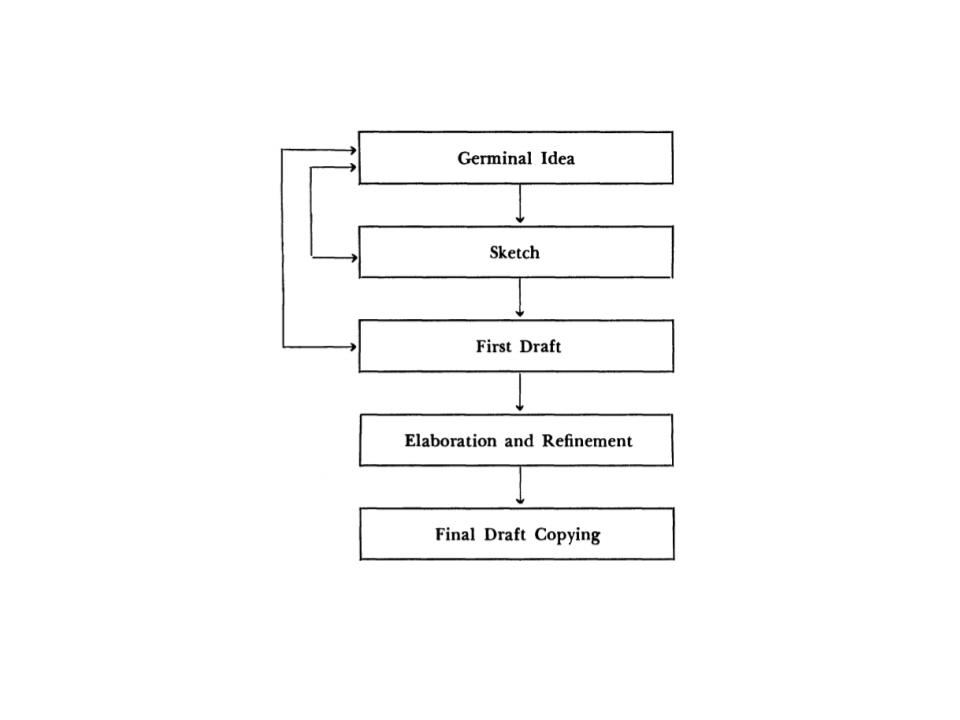
\includegraphics[width=12cm ]{figures/Composition.jpg}
    \caption{Stages of Music Composition \protect\cite{bennett1976process}}
    \label{fig:composition}
\end{figure}

\subsection{Music Fundamentals}
Music as defined in the study of \citeA{willoughby1971comprehensive}, is formed by combining the fundamentals of music. These fundamentals of music are discussed by \citeA{rivadelo1986fundamentals}. The author named the fundamentals as: rhythm, pitch, melody, texture and harmony, color and timbre, and form. 

In a composition, a sound can have a high or low tone which is related to the amount of vibrations per second, this is called pitch \cite{rivadelo1986fundamentals}. Pitches are represented by the first seven letters in the alphabet, namely A, B, C, D, E, F, and G \cite{miller2005complete}. The distances between a pitch from each other is illustrated as whole step, a half step, or semitone. In the keys of a piano or keyboard, moving from one key to a next key is called a half step or semitone respectively. A whole step was then described by \citeauthor{rivadelo1986fundamentals} as moving from one key to another and skipping the key between them. When adding the word up or down after the distance, half step, and whole step can traverse forward or backward. It is also possible to put a number before the distance in order to indicate multiple steps. 

Rhythm, as explained by \citeA{rivadelo1986fundamentals}, is made up of five distinguishable parts namely: clap, accent, meter, rhythmic pattern, and phrase. The clap is the key time unit used by the composition. The meter divides the claps into multiple sections. The accent is responsible for the formation of the theme of the rhythm. And lastly, the phrase is part of a musical thought, which is a component of the musical sentence.

Rhythm, as part of a composition, represents how fast or how slow the musical flow through the common patterns \cite{rivadelo1986fundamentals}. It is also understood that rhythm is the aspect that makes people aware of the tempo of the composition. It lets them adjust the ideas they have in order to add pitch and melody on top of the rhythm.

Another important component of a composition is the duration, which is basically the amount of time a tone or sound lasts \cite{rivadelo1986fundamentals}. This is seen in a composition in a staff through a note or rest. The type of note or rest indicates how long the duration of the pitch \cite{rivadelo1986fundamentals}. 

It is also important to note that rhythm depends on the tempo of the composition. The tempo defines the pace of the composition \cite{rivadelo1986fundamentals, nelson2009foundations}. Tempo is used by composers to set a mood or make the music more playable. Recently however, composers tend to use beats per minute to represent the tempo of a composition \cite{nelson2009foundations}.

There are seven common tempo markings according to \citeauthor{nelson2009foundations}. 
\begin{itemize}
    \item Grave, a very slow tempo. It has a bpm of around 25-40.
    \item Largo, a broad tempo. It has a bpm of around 40-60.
    \item Larghetto which is like largo but faster. It has a bpm of around 60-66.
    \item Adagio, a slow tempo but with great expression. It has a bpm of around 66-76.
    \item Andante, a walking pace tempo. It has a bpm of around 76-108.
    \item Moderato, a moderate speed tempo. It has a bpm of around 108-120.
    \item Allegro, a fast tempo it is also bright and quick. It has a bpm of around 120-156. 
\end{itemize}

FireflyX will be using these seven tempo markings to indicate the current tempo of the composition. The floor bpm of the tempo markings will be used to scale the speed of the composition.

\subsection{Musical Notation}
Musical notation is the method of visually representing musical sound \cite{read1964music}. Musicians use the notations to illustrate their musical ideas. As explained by \citeA{read1964music}, for people to be musically literate they would need to have an understanding of the symbols used in musical notation.

\begin{figure}[H]
    \centering
    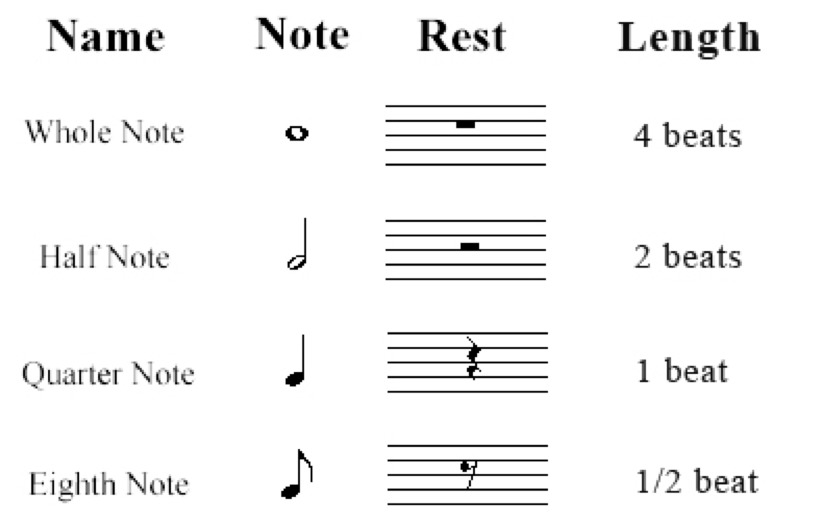
\includegraphics[width=10cm ]{figures/BasicMusicNotes.png}
    \caption{Basic notes and rests used in modern musical notation \protect\cite{BasicNotes2016}}
    \label{fig:BasicNotes2016}
\end{figure}

The notes and rests found in Figure \ref{fig:BasicNotes2016} are some of the basic symbols in musical notation. The symbol of the notes and rests represent how long a clap is. They staff is a set of lines and spaces which indicate the levels of pitches. The notes and rests are found throughout the staff, and their position on the staff represent their pitch. However, these pitches are also based on the clef found at the start of the staff. The G-clef as seen in figure \ref{fig:G-Clef} change the pitch represented by the staff. When it is used at the start of the staff, each line of the staff starting from the bottom represent the pitches E-G-B-D-F and the spaces represent the pitches F-A-C-E.

\begin{figure}[H]
    \centering
    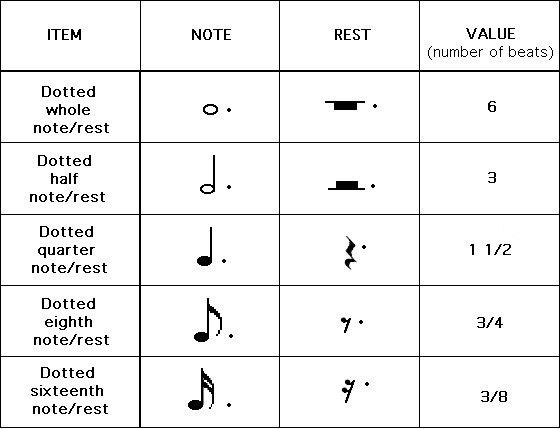
\includegraphics[width=10cm ]{figures/dotted_notes_chart.jpg}
    \caption{Dotted notations \protect\cite{DottedNotes2015}}
    \label{fig:DottedNotes2015}
\end{figure}

In addition to this, the duration of the note could be extended by putting a dot after the note. When a dot is added to the note, the duration of the note is increased by half of its original value. Multiple dots could be added and the subsequent dots add the progressively halved value. Examples of dotted notations and their equivalent duration can be found in Figure \ref{fig:DottedNotes2015}.

\begin{figure}[H]
    \centering
    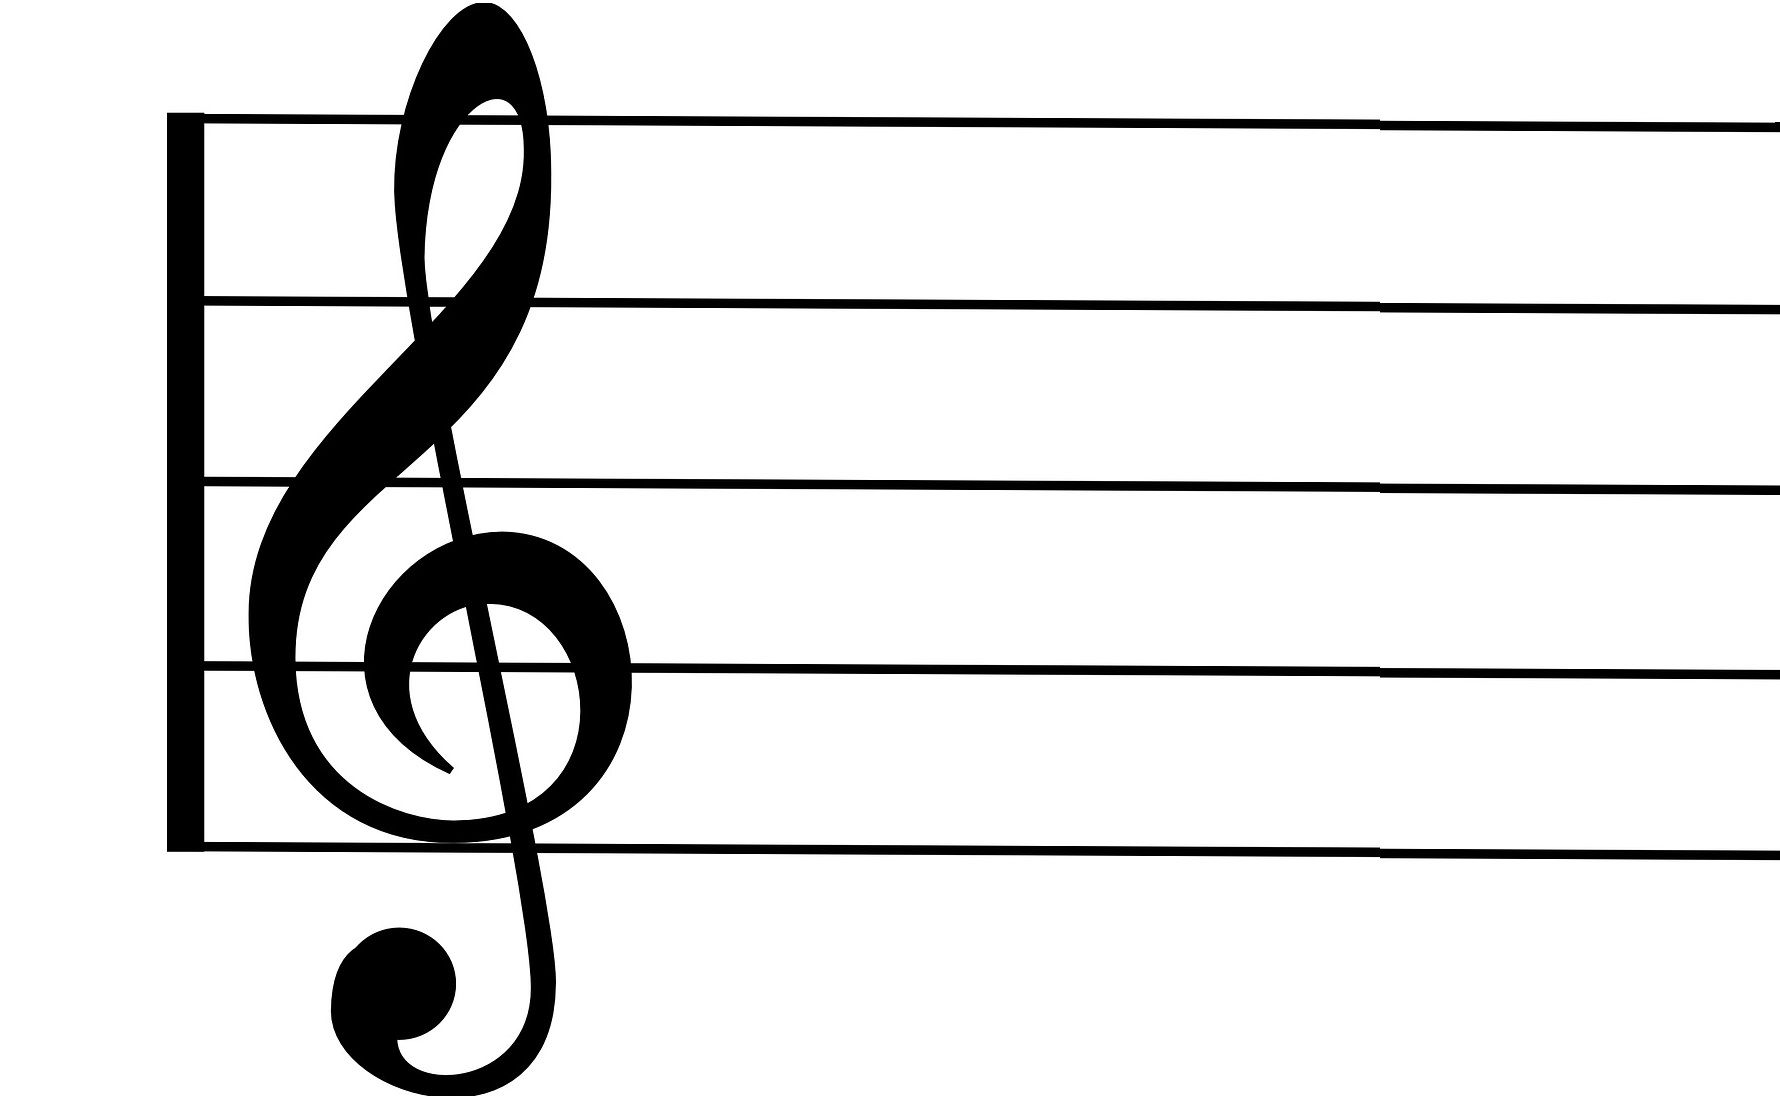
\includegraphics[width=5cm ]{figures/G-clef.jpg}
    \caption{The G-Clef \protect\cite{G-Clef}}
    \label{fig:G-Clef}
\end{figure}

The time signature defines the distinct rhythm throughout the composition \cite{rivadelo1986fundamentals}. As seen in figure \ref{fig:Time-Signature}, there are two numbers found in a time signature namely, the numerator and the denominator. In the time signature, the numerator always takes two spaces of the staff \cite{read1964music, rivadelo1986fundamentals, burrows1999read}.

\begin{figure}[H]
    \centering
    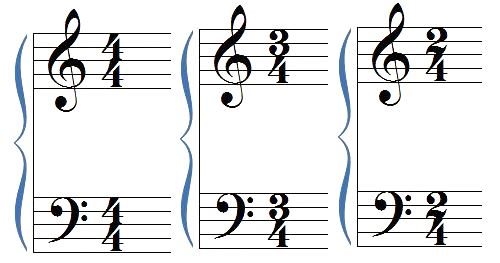
\includegraphics[width=7cm ]{figures/Time-Signature.jpg}
    \caption{The various time signatures \protect\cite{Time-Signature}}
    \label{fig:Time-Signature}
\end{figure}

The bar lines, as seen in figure \ref{fig:Bar-Lines} represent the division of notes in a musical sheet. There are two kinds of bar lines in musical compositions. The first kind of bar line is one vertical line that divides the notes based on the time signature of the staff. The second kind of bar line is the double bar line which is represented by two vertical lines. The double bar line is seen at the end of a composition \cite{read1964music}.  

\begin{figure}[H]
    \centering
    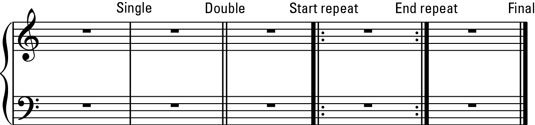
\includegraphics[width=9cm ]{figures/Bar-Lines.jpg}
    \caption{The various bar line notations \protect\cite{Bar-Lines}}
    \label{fig:Bar-Lines}
\end{figure}

\subsection{Music Language Synthesis}
Computer tools have recently been made to help in representing different elements of music, as natural languages are being made to help in representing the demands of music composition which will help in understanding music \cite{loy1985programming}.
\newline

One study aimed in making an open-ended programming language is the study of \citeA{dannenberg1997machine} named Nyquist. The study aimed to help in creating compositional tasks. By using Nyquist, sounds can be assigned into variables, stored into data structures, and can also be passed as parameters \cite{dannenberg1997machine}. In the study, musical composition can be represented as a series of sounds in a sequence and can be given arbitrary offsets. 

In Nyquist, expressions are written using Lisp \cite{turetsky1984lisp}, where parentheses define when applying a function to a set of parameters. An expression consists of variables and keywords. An example of an expression is seen in the expression \ref{NyquistExpression} where it simulates two notes. A reference of their keywords and representations could be seen in Table \ref{NyquistKeywords}.

\begin{equation}
          (sim (fminst\: g4\: 100) \\
        (fminst\: g4\: 100))
    \label{NyquistExpression}
\end{equation}


\begin{table}[H]
\centering
\label{NyquistKeywords}
\caption{Related Studies on Sandbox Environments and other Dynamic Interfaces \cite{dannenberg1997machine}}
\begin{tabular}{|l|l|} 
\hline
\textbf{Keyword in Nyquist}  & \textbf{Representation}                \\ 
\hline
defun                        & define function                        \\ 
\hline
at s t                       & shift sound s by t seconds in time     \\ 
\hline
seq                          & arranges sound sequentially            \\ 
\hline
sim                          & arranges sound simultaneously          \\ 
\hline
scale                        & scales sound to a different amplitude  \\ 
\hline
play                         & plays the sound                        \\ 
\hline
fminst                       & pitch depth                            \\
\hline
\end{tabular}
\end{table}

A thesis by \citeA{ince2019programming} also emphasized in the use of patterns in representing music as they described them as events in time. Where these structures of music can be formed into a sequence of events, as this idea is used in specifying the music pattern in a language. Their application named Siren emphasizes on the creation of these patterns as they found inspiration from Haskell a pattern language, which generates a \say{library of patterns} to represent music \cite{ince2019programming}.

FireflyX will be implementing clap-rest patterns that will represent the parts of the firefly model. Techniques in the work of Nyquist specifically music as a set of parameters will be implemented for the program to read the configuration from an XML file. The configuration will then be parsed by a playback module and produce sound.


% The goal of Nyquist is to
% provide an open-ended programming language that
% supports high-level compositional tasks in addition
% to low-level signal processing.
% Sounds are first-class types in Nyquist;
% hence they can be assigned to variables, passed as
% parameters, and stored in data structures.
% Composition requires that sounds be placed simultaneously, in sequence, and at arbitrary offsets.

% For example, the expression
% (osc c4)
% means "apply the function osc to the parameter
% c4." Parameters are evaluated first. In this case, c4
% is a global variable (intended to remain constant)
% containing the value 60.0. The value 60.0 is passed
% to the osc function, and the result is a sinusoid
% whose frequency corresponds to middle C and
% whose duration is 1 sec.



%\section{Children's Learning}

%The early years in a child's life are important for learning. It is because learning is dependent on the plasticity of the brain which is strongest in those early years. This learning can stimulate brain growth and improve fine motor coordination \cite{gruhn2005children}. Learning on its own happens without people's consciousness. When listening to music, people process a lot of information.\cite{hallam2010power} These processed information leads to possible improvement in different fields such as mathematics, reading, and IQ in general \cite{vcrnvcec2006cognitive}. 
%
%A study by \cite{leung2010students} mentions that in Hong Kong, the music curriculum is aimed to teach students to develop in certain fields. One field to be developed is creativity and imagination. Another is the aim to develop skills and processes. Both of these can be developed by direct musical activities such as instrument playing and singing. During this process of learning, students are encouraged to act independently as they solve musical challenges so that one day they may become confident in solving problems in their daily lives.
%challenges
%Studies suggest however that even with its benefits, there are some challenges that come with it. One study \citeauthor{russell2009me} mentions of different things that public schools in order to teach music properly. The lack of knowledge, time, priority, experience, and resources are the main causes of public schools being unable to teach music properly. Teachers with the lack of knowledge of syllabus requirements and the lack of personal experience make them unable to teach properly. This also goes for the lack of time to prepare and to teach making the music lesson lacking.  The is usually also caused by the school not giving musical lessons any priority which also leads to the lack of resources to teach music with. 
%
%Another study by \citeauthor{may2013public}, mentions that the teachers must optimize the class environment for the music classes. For children, play is primary means of education as it something they are motivated to do on their own. A good music classroom would be one with an array of instruments for children to play with and explore.


%
%Interaction Design


% \section{User Research}
% \subsection{Experiment Design}


               %-- includes LaTeX source file for Chapter 3: Theoretical Framework
%                                   %-- your job: **EDIT THIS FILE** to indicate your research methodology

%%%%%%%%%%%%%%%%%%%%%%%%%%%%%%%%%%%%%%%%%%%%%%%%%%%%%%%%%%%%%%%%%%%%%%%%%%%%%%%%%%%%%%%%%%%%%%%%%%%%%%
%
%   Filename    : chapter_4.tex 
%
%   Description : This file will contain your Research Methodology.
%                 
%%%%%%%%%%%%%%%%%%%%%%%%%%%%%%%%%%%%%%%%%%%%%%%%%%%%%%%%%%%%%%%%%%%%%%%%%%%%%%%%%%%%%%%%%%%%%%%%%%%%%%

\chapter{Research Methodology}
% This chapter lists and discusses the specific steps and activities that will be performed by the proponent to accomplish the project. 
% The discussion covers the activities from pre-proposal to Final Thesis Writing.  It also includes an initial discussion on the theoretical
% framework to be followed.

% \section{Research Activities}
% Research activities include inquiry, survey, research, brainstorming, canvassing, consultation, review, interview, observe, experiment, design, 
% test, document, etc.  The methodology also includes the following information:

% \begin{itemize}
%   \item who is responsible for the task
%   \item the resource person to be contacted
%   \item what will be done
%   \item when and how long will the activity be done
%   \item where will it be done
%   \item why should be activity be done
% \end{itemize}

\begin{figure}[H]
    \centering
    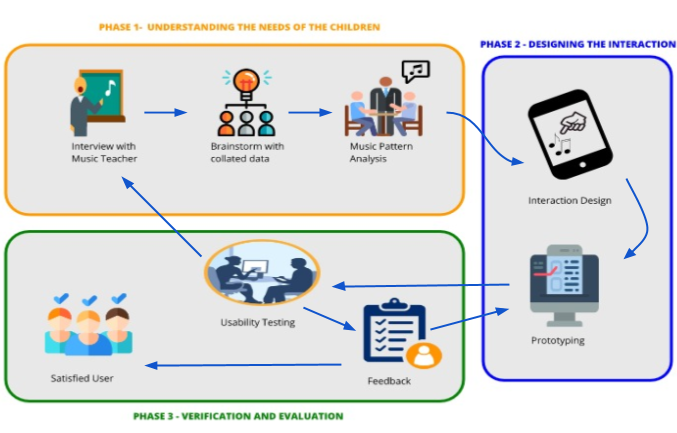
\includegraphics[width=16cm]{figures/Diagram1.png}
    \caption{Research framework for FireflyX}
    \label{fig:FireflyX}
\end{figure}

The methodology for this study can be divided into 3 phases. The first phase (see figure \ref{fig:FireflyX} Phase 1), aims to understand the students and identify their needs with the help of their music teacher. Using the data gathered from the interview with the teachers, the next phase (see figure \ref{fig:FireflyX} Phase 2) involves the designing of the interaction to solve the needs of the students. In the last phase (see figure \ref{fig:FireflyX} Phase 3) is a constant process of testing and developing on the proposed solution based on the feedback gathered in each tests.

% \section{Observation of Children Learning Music}
% Observing children while they are learning music is necessary to understand the process behind it. We will be doing this for at least 1 week in a music school for children aged 7-9 in the span of an hour. We will be using their classroom where they usually hold their music classes to conduct the observation. The activity will be recorded with a camera and a voice recorder for backup in case the camera fails. All members will take notes on a notebook of the interactions of the students and the teacher. By doing these, we can also ensure that we can properly optimize and cater our app for children learning. The main goal of this activity is to find points that we can improve on and find problems or difficulties that children are experiencing.

\section{Interview with the Music Teacher}
An interview with the music teacher of the children was done in order to understand the process of how children are taught music. The interview served as confirmation for the observations we made in the previous activity. This interview will also expand our knowledge on music and identify aspects that might not have been covered by previous observations. The interview was conducted in a secluded room where only the interviewer and the interviewee are present in order to minimize distractions in addition to this, a backup voice recorded. Observations was also written down on a notebook. The notes taken during the interview was used for discussion within the group to collate and brainstorm.

The main questions asked in the interviews are:
\begin{enumerate}
    % \item What are your thoughts on children and music?
    % \item Have you taught or are teaching anyone music?
    % \item Have you taught or are teaching children?
    %     If yes to both,
	   %     Have you taught or are teaching music to children?
    % \item What music concepts do you usually teach children ages of 5-8?
    % \item How would you teach these concepts to these children?
    % \item Do you think that the children are learning these concepts?
    % \item Is it difficult to teach music?
    % \item What about for teaching music to children?
    % \item What makes it different when teaching children?
    % \item What difficulties do children usually encounter when learning music?
    % \item What techniques or methods did you use to overcome these difficulties?
    % \item How do you suggest children should learn music?
    % \item What are signs that a child is learning a music concept?
    % \item Do you conduct tests?
    % \item If yes, what kind of tests do you conduct? If no, how do you evaluate if a child is learning music?
    % \item Do you have any suggestions on how to interact with children?
    \item How long have you been teaching music?
    \item Have you thought or are teaching children?
    \item How do you start your sessions with children?
    \item Do you have special techniques when teaching children?
    \item Do you use the same techniques with all the children?
    \item What difficulties do you encounter when you teach children?
    \item Do you keep in contact with the student outside the classroom?
    \item What role do the parents have in the learning journey of the child?
\end{enumerate}

The questions above are non-exhaustive and may lead to more follow up questions. Different questions may be inserted or added depending on how the musician would answer a question to gather more data or insights.

\section{Brainstorming on Collated Data}
After the observation and interview, it is necessary that we analyze and process the data acquired through a meeting. All data gathered was stored on a Google Drive and a flash drive for backup in case of lost files. Based on the problem statement, we then developed ideas and shared these ideas among ourselves. The group then tried to synthesize and improve on each idea. A scenario map was made based on how the teachers perceive the learning experience of children. The scenario map highlights the process of the children using the app. Personas were also made in order to identify which helps us identify the specific needs of the personas and better suit the prototype and app in order to cater the personas. The resulting list of features and solutions would then be consulted to a music expert to determine if a prototype will be possible or usable for children.

% \section{Consulting with Music Expert}
% % An interview with a music expert will be done in order to understand the process of how children understand music. The interview will also help us validate and confirm the observations we made in the previous activity. This interview will also expand our knowledge on music theories and also to identify aspects that might not have been covered by previous observations. Like the interview with the music teacher, the interview will be conducted in a secluded room, recorded by camera and voice. Observations will also be taken note of and finally the notes taken during the interview will be used for discussion within the group to collate and brainstorm.
% Once the team has finished brainstorming on potential solutions, we would set an interview with the music expert. This is done as we would want to verify what the teacher said to us during the interview and how the children acted during our observation of them. Also we would want to know if the data gathered is true based on musical theory. For the consideration of our music expert we would want him/her to have many experiences on the field of music and also children. 

The main questions asked in the consultation are:
\begin{enumerate}
    \item Have you taught music to children of age 5-8?
    \item What are the musical theories that children of age 5-8 should be learning?
    \item What are some of the difficulties in teaching music to children?
    \item How did you overcome these difficulties?
    \item Do you have any suggestions on how to interact with children?
    \item How did you assess the learning of the children?
    \item Were the observations we made on the children accurate?
    \item What areas are important to observe when conducting activities with children?
    \item Was the assessment of the teacher based on our observation of the children accurate?
    \item What are some suggestions you can give on how we should design our system based on our observations?
    \item Do you have any suggestions on what features would be important for the app?
\end{enumerate}

The questions above are non-exhaustive and may lead to more follow up questions. Different questions may be inserted or added depending on how the musician would answer a question to gather more data or insights.

\section{Music Pattern Analysis}
Rhythmic music patterns acquired from the Suzuki Book 1 will be analyzed. The most frequent clap-reset combination was taken into account and included in the Library of Patterns (Refer to Table \ref{Patterns}). We also looked at music sheets for piano to help us in modeling patterns found with the integration of different pitches. We took inspiration from the idea of Nyquist to make these patterns and represent them in Swift. This also gave us an idea on which claps and notes would be used for the mapping of the firefly model. Included in this would be the amount of claps per measure, measures per section, and the amount of sections per rhythm. All of these will be considered when deciding on the possible firefly configurations.

\section{Interaction Design and Prototyping}
Using the input given by the teacher and music expert, concepts for the initial interaction design are to be sketched out on paper. The sketches will be based on how the mapping of the firefly model will be, and from the features developed from the previous activities. The sketches will also be tested first by the teacher before being implemented into a mockup. Feedbacks and suggestions will also be gathered to improve the sketches and mockups. Multiple designs are to be created based on how each member's ideas on how to solve the problems of the students. 

Once a design was agreed upon by each member of the group, a mid-fidelity prototype is to be made using Figma to design for the proposed interface of the app based on the observation, interview, and consultations done in the previous activities. The decisions for the mappings of the firefly will also be decided in this part. The music patterns analyzed from the activity before will be used here to decide which features from the music patterns will be mapped to a firefly part. Music fundamentals like rhythm, tempo and pitch will also be mapped to a specific firefly part.

Like the activities before, feedback will be gathered in order to improve the prototype. Even though there will be limited functionality and features in the prototype, this will give us a better idea before developing the actual app.

\section{Implementing and Testing the Prototypes}
An agile software development methodology will be implemented. The software engineering approach will be iterative, where we will take into account the feedback and suggestions of the users to improve the next iteration. A GitHub repository will be created to store and to have save points for the prototype. The prototype will be updated every time after we analyze and collate the data. Updates will be pushed to a GitHub repository when we have decided on a proper update. The GitHub repository will also serve as an access point for the members of the group. 

After developing the app, usability tests will be performed with the objective of determining the overall experience in using the app. Before starting the test, the testers will first be given a consent form along as the consent from their parents. If they agree with the terms and decided to continue with the testing, they will be given a brief introduction and description of the study along with the objectives and overview. They will then be asked to use Firefly and be assessed after. During the test we will encourage the child to think aloud as this will help us in gathering more inputs on the human factors they exhibit in doing the tasks. For the test setup these will be conducted where there is little to no audio and visual distractions. This will ensure that the users will be focused, and also to maintain the clear audio and video while recording. The latest version of firefly installed in a tablet iPad will be provided to the tester of the application. There will be two cameras recording the tester, the first is the camera of the laptop that records the facial expressions. This will be needed to see the reactions of the tester. The second camera records the gestures with the interaction with the application. The tasks will be written on a piece of paper that is visible for the child to see in the table. These will all be recorded using an audio recording device to capture the audio to be used for the transcription of the user testing. 

The evaluation for the test will be digital and will be operated by the test moderator. The test moderator will ask the child questions and will then record the answers of the child in the form. The quantitative data will also be acquired in the evaluation mentioned earlier. This form of data is to be used in evaluating the usability data of the applications different features. This is done by the group to identify the features that have caused inconveniences for the users. The data will then be analyzed to improve the app and factor in the feedback acquired from the testing. Sample questions will be written in the different iterations of testing below. Interviews will also be done after the testing to validate the observations and also to get feedback on the user experience of the children testing the application. The adult companion and the teacher will be able to accompany and watch the child during testing.

For the first and second iteration it will be following the diagram shown in figure \ref{test1and2}.

\begin{figure}[H]
    \centering
    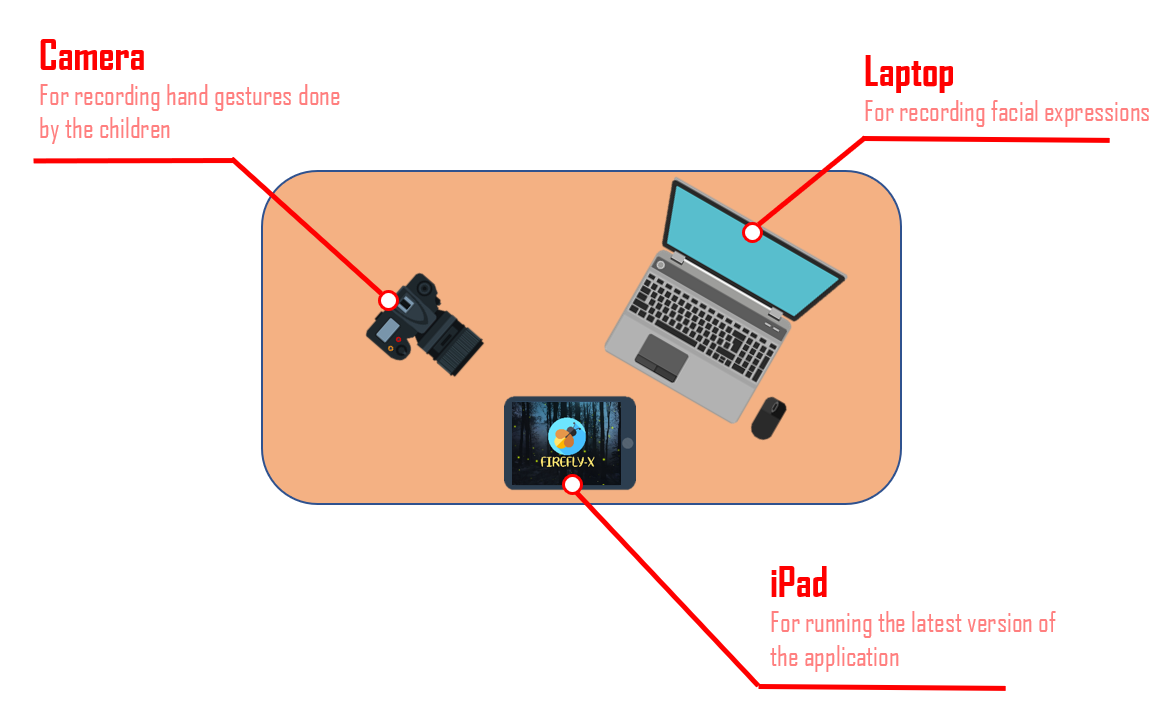
\includegraphics[width=15cm]{figures/Test_Setup.png}
    \caption{Iteration 1 and 2 Test Setup}
    \label{test1and2}
\end{figure}

The testers, music students aged 5-8 from different music schools will be asked to take part in the data collection and testing. Testing will be divided into three (3) phases with each iteration having a set of different tasks since more features are to be added in the application per iteration. 

Tasks that will be asked to do will be modeled from the use cases found in Appendix \ref{sec:appendixc}.

\subsection{First Iteration}
After developing the application which is 60\% complete, it would be tested with three (3) users. Since the functionality at this iteration is still at 60\%, we would like the users to test mainly on the fundamental functionality with only one firefly. These tasks revolve around the manipulation of the parts/functionality of the firefly. To meet 60\% completeness namely the tail (pattern), wing (repetition), body (tempo), wing (note speed), and the playback engine. 

These are examples of tasks that will be asked to be done for the first iteration:
\begin{itemize}
    \item Set the tempo of the firefly by choosing a body type
    \item Set the number of repetitions of the firefly by choosing a setting in the right wing
    \item Set the speed of note of the firefly by choosing a setting in the left wing
    \item Set the blinking pattern of the firefly by choosing a tail type
    \item Replace the tempo by selecting a different body type
    \item Replace the current repetition by selecting a different setting in the left wing
    \item Replace the current speed of note by selecting a different setting in the right wing
    \item Replace the pattern by selecting a different tail type
    \item Tap start to start playing the firefly
    \item Tap stop to stop the firefly from playing
    \item Tap on the power button to exit to main menu
\end{itemize}

These are the sample questions in the evaluation with the scale being 1 being the easiest to 5 being difficult. We will be asking these to tester to better understand the functionality of the first iteration:

\begin{itemize}
    \item How difficult was it to set the tempo? 
    \item How difficult was it to set the repetition? 
    \item How difficult was it to set the speed of the note? 
    \item How difficult was it to set the clap-rest pattern? 
    \item How difficult was it to replace the current tempo? 
    \item How difficult was it to replace the current repetition? 
    \item How difficult was it to replace the current speed of the note? 
    \item How difficult was it to replace the current clap-rest pattern? 
    \item How difficult was it to start playing the firefly?
    \item How difficult was it to stop to stop the firefly from playing?
    \item Was it difficult to go through the application?
    \item Do you like the design of the application?
    \item Was the functionality of the parts clearly seen?
\end{itemize}

\subsection{Second Iteration}
In the second iteration we would then test the application that is 80\% complete with seven (7) testers. From the seven testers three of them will be retained from the first iteration of testing, meaning we would have four new participants for this iteration. In this iteration we will be implementing the changes based on the comments received from the first iteration of testing. The aim is to be 80\% wherein there will still be one firefly playing. Functionalities such as pitch and release to canvas, in addition with the ability to manipulate the firefly parts will be added to meet the 80\% completeness.

The tasks from the first iteration will carry on in the second iteration testing. These are examples of newly added tasks that will be asked to be done for the second iteration:
\begin{itemize}
    \item Tap pause to pause the firefly from playing 
    \item Tap resume to resume the playing of the firefly
    \item Tap the jar to replay previous fireflies 
    \item Tap on the Feed Me Button to start changing the pitch
    \item Set the pitch of each note by dragging the biscuit on the tray to the staff
    \item Start replacing the current pitch of a note by clicking Feed Me button again
    \item Replace the current pitch for one or more notes by dragging the biscuit/s to a higher line in the staff
    \item Replace the current pitch for one or more notes by dragging the biscuit/s to a lower line in the staff
    \item Clear the pitch for all notes by selecting the Clear button 
    \item Preview the pitch representation of the firefly by selecting the Preview button 
\end{itemize}

These are the sample questions in the evaluation with the scale being 1 being the easiest to 5 being difficult. Aside from the questions that we will ask again that came from iteration 1 we will be introducing these new questions to the tester to better understand the functionality of the second iteration:

\begin{itemize}
    \item How difficult was it to pause the firefly from playing?
    \item How difficult was it to resume the playing of the firefly?
    \item How difficult was it to to replay previous fireflies?
    \item How difficult was it to set the pitch? 
    \item How difficult was it to replace the current pitch to a higher position in the staff? 
    \item How difficult was it to replace the current pitch to a lower position in the staff?
    \item How difficult was it to clear all pitches? 
    \item How difficult was it to preview the pitch playback? 
\end{itemize}

\subsection{Third Iteration}
Lastly in the third iteration, fifteen (15) users will be testing the complete application. Where same as the second iteration we will retain the seven users that already have tested the application previously and we will get eight new participants in this last iteration. The last stage revolves on improving the functionality from the first two stages. Functionality in this stage for it to be fully complete should already handle five (5) fireflies as well as saving and loading the workspace. The tasks will also use the same as the first two iterations and also adding the new functionality developed in this last iteration. For the last iteration since new tasks on composing will be added we will be also adding a music sheet in the test setup as seen in figure \ref{test3}.

\begin{figure}[H]
    \centering
    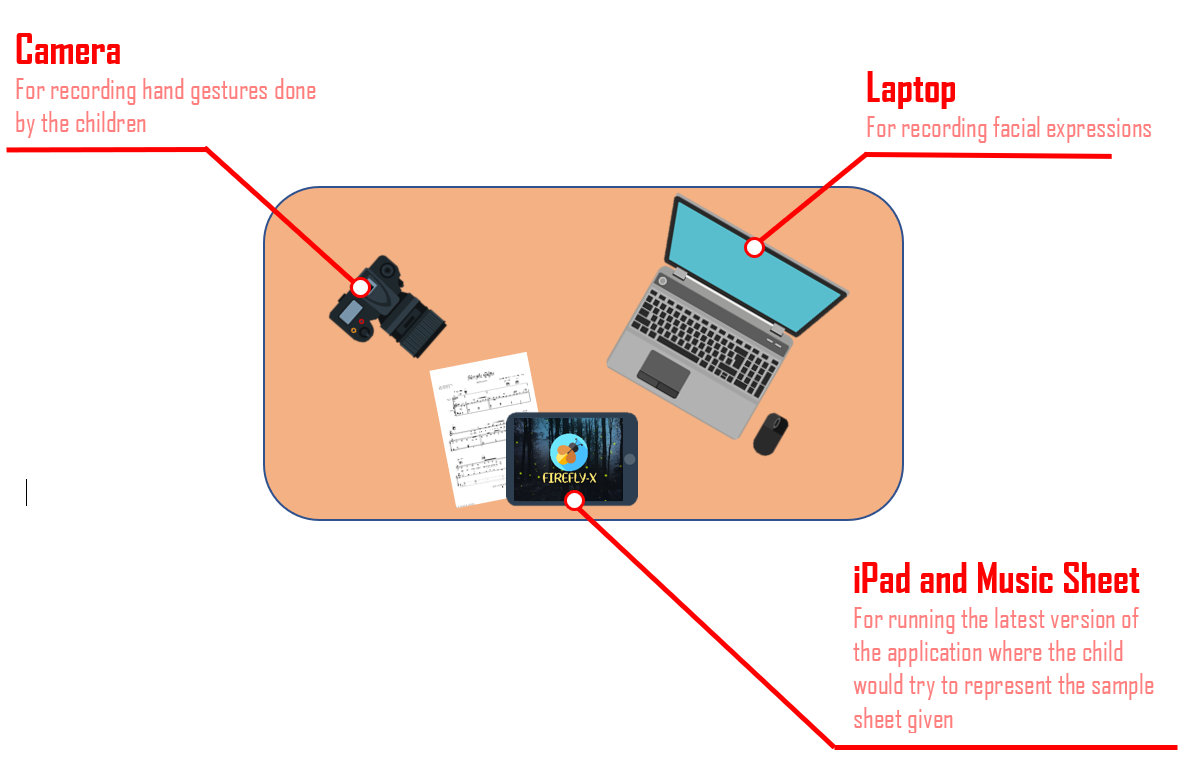
\includegraphics[width=15cm]{figures/Test_Setup_Last.png}
    \caption{Iteration 3 Test Setup}
    \label{test3}
\end{figure}

The tasks from the first and second iteration will carry on in the third iteration testing. These are examples of newly added tasks that will be asked to be done for the third iteration:
\begin{itemize}
    \item Tap Reset Album to reset the fireflies
    \item Tap Save to save the modified fireflies
    \item Tap Load to load previously made fireflies
    \item Configure the fireflies to emulate a sample sheet given by the testers (Hot Cross Buns)
    \item Configure the fireflies to make a simple familiar song like (Twinkle Twinkle Little Star/Happy Birthday)
    \item Edit the fireflies to modify a previously made track
    \item Free play of the environment
    \item Configure five fireflies
\end{itemize}

These are the sample questions in the evaluation with the scale being 1 being the easiest to 5 being difficult. Aside from the questions that we will ask again that came from iteration 1 we will be introducing these new questions to the tester to better understand the functionality of the second iteration:

\begin{itemize}
    \item How difficult was it to to reset the fireflies?
    \item How difficult was it to save the modified fireflies?
    \item How difficult was it to load previously made fireflies?
    \item How difficult was it to copy the sample sheet Hot Cross Buns using the fireflies? 
    \item How difficult was it to modify a previously made track? 
    \item How difficult was it to freely play the application?
    \item How difficult was it to configure the five fireflies in an environment?
    \item How would you rate the learning you got from the application?
\end{itemize}

% Sample questions asked in different iterations of feedback from the users:
% \begin{enumerate}
%     \item How much did you use this feature to accomplish the tasks?
%     \item On a scale of 1 to 4 (with 4 being the highest and 1 being the lowest) were you comfortable while using this feature?
%     \item Is there any need to improve this feature? Why?
% \end{enumerate}

% \section{Usability Testing}

% \section{Feedback}
% The feedback from testing will come in forms of qualitative and quantitative data. Qualitative data will be acquired through video recordings, observations, and interviews. The setup will include cameras to capture the facial expressions and hand gestures while the children are testing the application. Interviews will also be done after the testing to validate the observations and also to get feedback on the user experience of the children testing the application. The quantitative data will also be acquired in forms of a questionnaire. This form of data is to be used in evaluating the usability data of the applications different features. This is done for the group to identify the features that have caused inconveniences for the users. A scale from 1-4 will be asked from the testers with the assistance of the teacher with 4 being the highest and 1 being the lowest. 



\begin{landscape}
\section{Gantt Chart}
% \begin{table}[H]
% \centering
% \caption{Timetable of Activities} \vspace{0.25em}
% \begin{tabular}{|l|l|l|l|l|l|l|l|l|l|l|l|l|l|l|l|l|}
%     \hline
%     2019 - 2020                  & May  & Jun   & July & Aug  & Sep & Oct & Nov & Dec & Jan  & Feb  & Mar  & Apr & May  & Jun  & Jul  & Aug \\ \hline
%     Planning                     & \textbullet    & \textbullet     & \textbullet    & \textbullet    & ~   & ~   & ~   & ~   & ~    & ~    & ~    & ~   & ~    & ~    & ~    & ~   \\ \hline
%     RRL & \textbullet\textbullet\textbullet\textbullet & \textbullet\textbullet\textbullet\textbullet & \textbullet\textbullet\textbullet\textbullet & \textbullet\textbullet\textbullet\textbullet & ~   & ~   & ~   & ~   & ~    & ~    & ~    & ~   & ~    & ~    & ~    & ~   \\ \hline
%     Learning Swift      & ~    & ~     & \textbullet\textbullet\textbullet & \textbullet\textbullet\textbullet  & \textbullet\textbullet  & \textbullet   & \textbullet   & ~   & ~    & ~    & ~    & ~   & ~    & ~    & ~    & ~   \\ \hline
%     Development                  & ~    & ~     & ~    & ~    & ~   & \textbullet\textbullet\textbullet\textbullet   & \textbullet\textbullet\textbullet\textbullet   & \textbullet\textbullet\textbullet  & \textbullet\textbullet\textbullet\textbullet & \textbullet\textbullet\textbullet\textbullet & \textbullet\textbullet\textbullet\textbullet & \textbullet\textbullet  & ~    & ~    & ~    & ~   \\ \hline
%     Experiment Design              & ~    & ~     & ~    & ~    & ~   & ~   & ~   & ~   & ~    & \textbullet    & \textbullet\textbullet   & \textbullet\textbullet  & ~    & ~    & ~    & ~   \\ \hline
%     Results and Analysis         & ~    & ~     & ~    & ~    & \textbullet \textbullet   & \textbullet \textbullet \textbullet \textbullet   & \textbullet   & ~   & ~    & ~    & ~    & \textbullet\textbullet\textbullet & \textbullet\textbullet\textbullet\textbullet & \textbullet\textbullet\textbullet\textbullet & ~    & ~   \\ \hline
%     Documentation                & \textbullet    & \textbullet     & \textbullet    & \textbullet    & \textbullet   & \textbullet   & \textbullet   & \textbullet   & \textbullet    & \textbullet    & \textbullet    & \textbullet   & \textbullet\textbullet   & \textbullet\textbullet\textbullet\textbullet & \textbullet\textbullet\textbullet\textbullet & \textbullet   \\ \hline
% \end{tabular}
% \label{tab:ganttChart}
% \end{table}
% Please add the following required packages to your document preamble:
% \usepackage[normalem]{ulem}
% \useunder{\uline}{\ul}{}
\begin{table}[H]
\caption{Timetable of Activities} \vspace{0.25em}
\label{tab:ganttChart}
\begin{tabular}{|l|l|l|l|l|l|l|l|l|l|l|l|l|l|l|l|l|}
\hline
2019 - 2020                                                                & May                                                                                                      & Jun                                                                                                      & July                                                                                                     & Aug                                                                                                      & Sep                                                                                                      & Oct                                                                                                         & Nov                                                                                                      & Dec                                                                            & Jan                                                                                                      & Feb                                                                                                      & Mar                                                                                                      & Apr                                                                            & May                                                                                                      & Jun                                                                                                      & Jul                                                                                                      & Aug                        \\ \hline
Planning                                                                   & \textbullet                                                                               & \textbullet                                                                               & \textbullet                                                                               & \textbullet                                                                               &                                                                                                          &                                                                                                             &                                                                                                          &                                                                                &                                                                                                          &                                                                                                          &                                                                                                          &                                                                                &                                                                                                          &                                                                                                          &                                                                                                          &                            \\ \hline
RRL                                                                        & \textbullet\textbullet\textbullet\textbullet & \textbullet\textbullet\textbullet\textbullet & \textbullet\textbullet\textbullet\textbullet & \textbullet\textbullet\textbullet\textbullet &                                                                                                          &                                                                                                             &                                                                                                          &                                                                                &                                                                                                          &                                                                                                          &                                                                                                          &                                                                                &                                                                                                          &                                                                                                          &                                                                                                          &                            \\ \hline
Interview                                                                  &                                                                                                          &                                                                                                          &                                                                                                          &                                                                                                          & \textbullet\textbullet\textbullet\textbullet & \textbullet                                                                                  &                                                                                                          &                                                                                &                                                                                                          &                                                                                                          &                                                                                                          &                                                                                &                                                                                                          &                                                                                                          &                                                                                                          &                            \\ \hline
\begin{tabular}[c]{@{}l@{}}Preliminary Results\\ and Analysis\end{tabular} &                                                                                                          &                                                                                                          &                                                                                                          &                                                                                                          &                                                                                                          & \textbullet\textbullet\textbullet\textbullet    &                                                                                                          &                                                                                &                                                                                                          &                                                                                                          &                                                                                                          &                                                                                &                                                                                                          &                                                                                                          &                                                                                                          &                            \\ \hline
Learning Swift                                                             &                                                                                                          &                                                                                                          &                                                                                                          &                                                                                                          &                                                                                                          &                                                                                                             & \textbullet\textbullet\textbullet\textbullet                                                                               &  \textbullet\textbullet                                                                             &      \textbullet\textbullet\textbullet\textbullet                                                                                                    &                                                                                                          &                                                                                                          &                                                                                &                                                                                                          &                                                                                                          &                                                                                                          &                            \\ \hline
Development                                                                &                                                                                                          &                                                                                                          &                                                                                                          &                                                                                                          &                                                                                                          & \textbullet\textbullet\textbullet\textbullet    & \textbullet\textbullet\textbullet\textbullet & \textbullet\textbullet\textbullet & \textbullet\textbullet\textbullet\textbullet & \textbullet\textbullet\textbullet\textbullet & \textbullet\textbullet\textbullet\textbullet & \textbullet\textbullet                           &                                                                                                          &                                                                                                          &                                                                                                          &                            \\ \hline
Experiment Design                                                          &                                                                                                          &                                                                                                          &                                                                                                          &                                                                                                          &                                                                                                          &                                                                                                             &                                                                                                          &                                                                                &                                                                                                          & \textbullet                                                                               & \textbullet\textbullet                                                     & \textbullet\textbullet                           &                                                                                                          &                                                                                                          &                                                                                                          &                            \\ \hline
Results and Analysis                                                       &                                                                                                          &                                                                                                          &                                                                                                          &                                                                                                          & \textbullet \textbullet                                                    & \textbullet \textbullet \textbullet \textbullet & \textbullet                                                                               &                                                                                &                                                                                                          &                                                                                                          &                                                                                                          & \textbullet\textbullet\textbullet & \textbullet\textbullet\textbullet\textbullet & \textbullet\textbullet\textbullet\textbullet &                                                                                                          &                            \\ \hline
Documentation                                                              & \textbullet                                                                               & \textbullet                                                                               & \textbullet                                                                               & \textbullet                                                                               & \textbullet                                                                               & \textbullet                                                                                  & \textbullet                                                                               & \textbullet                                                     & \textbullet                                                                               & \textbullet                                                                               & \textbullet                                                                               & \textbullet                                                     & \textbullet\textbullet                                                     & \textbullet\textbullet\textbullet\textbullet & \textbullet\textbullet\textbullet\textbullet & \textbullet \\ \hline
\end{tabular}
\end{table}
\end{landscape}

% \section{Calendar of Activities}

% A Gantt chart showing the schedule of the activities should be included as a table. For example:

% Table \ref{tab:timetableactivities} shows a Gantt chart of the activities.  Each bullet represents approximately
% one week worth of activity.

%
%  the following commands will be used for filling up the bullets in the Gantt chart
%
\newcommand{\weekone}{\textbullet}
\newcommand{\weektwo}{\textbullet \textbullet}
\newcommand{\weekthree}{\textbullet \textbullet \textbullet}
\newcommand{\weekfour}{\textbullet \textbullet \textbullet \textbullet}

%
%  alternative to bullet is a star 
%
\begin{comment}
   \newcommand{\weekone}{$\star$}
   \newcommand{\weektwo}{$\star \star$}
   \newcommand{\weekthree}{$\star \star \star$}
   \newcommand{\weekfour}{$\star \star \star \star$ }
\end{comment}



% \begin{table}[ht]   %t means place on top, replace with b if you want to place at the bottom
% \centering
% \caption{Timetable of Activities} \vspace{0.25em}
% \begin{tabular}{|p{2in}|c|c|c|c|c|c|c|c|} \hline
% \centering Activities (2009) & Jan   & Feb & Mar & Apr & May & Jun & Jul \\ \hline
% Study on Prerequisite Knowledge      &   &  & ~~~\weektwo & \weekfour &  &  &  \\ \hline
% Review of Existing Racing Strategies & ~~~\weektwo  & \weekfour & \weekfour & \weekfour &  &  &  \\ \hline
% Identification of Best Features      &   &  &  & \weekfour & \weektwo~~~ &  &  \\ \hline
% Development of Racing Strategies     &   &  &  & ~~~\weektwo & \weekfour & \weektwo~~~ &  \\ \hline
% Simulation of Racing Strategies      &   &  &  & ~~~\weektwo & \weekfour & \weekthree~~ &  \\ \hline
% Analysis and Interpretation of the Results &   &  &  &  & \weekfour & \weekfour & \weekone~~~~~ \\ \hline
% Documentation & ~~~\weektwo  & \weekfour & \weekfour & \weekfour & \weekfour & \weekfour & \weektwo~~~ \\ \hline
% \end{tabular}
% \label{tab:timetableactivities}
% \end{table}

               %-- includes LaTeX source file for Chapter 4: Research Methodology
%                                   %-- your job: **EDIT THIS FILE** to indicate your research methodology

%%%%%%%%%%%%%%%%%%%%%%%%%%%%%%%%%%%%%%%%%%%%%%%%%%%%%%%%%%%%%%%%%%%%%%%%%%%%%%%%%%%%%%%%%%%%%%%%%%%%%%
%
%   Filename    : chapter_5.tex 
%
%   Description : This file will contain your System Design.
%                 
%%%%%%%%%%%%%%%%%%%%%%%%%%%%%%%%%%%%%%%%%%%%%%%%%%%%%%%%%%%%%%%%%%%%%%%%%%%%%%%%%%%%%%%%%%%%%%%%%%%%%%

\chapter{System Design}

\section{System Overview}
FireflyX is a mobile application tool that aims to aid children in learning music fundamentals. There will only be one role, which is the user. The target users are children of ages 5 to 8 with little knowledge of music. The user may edit the firefly models' parts based on their preferences.

The properties of the rhythm that can be configured on the firefly model are the tempo, length of the note, repetitions, rest pattern, and pitch. Each part of the firefly model directly corresponds to one property that can be modified.

The parts of the firefly model may be configured either by part or by manipulating the parts by gestures, such as pinching, swiping, and tapping. After a firefly model is configured, the user may set it free on a canvas where they can freely fly and roam. The rhythm will then be played with the properties set by the different parts the user has chosen or have tweaked. 

In order to create a rhythm, the user is allowed to make more firefly models with different configuration. The user will be allowed to play, pause, reset, stop, and save their current workspace.

\section{System Objectives}
The system aims to accomplish the following:
\begin{itemize}
    \item To enable users to make a rhythm and pitch using firefly models.
    \item To allow users to change the properties of the rhythm and pitch by tweaking the parts of the firefly model.
    \item To allow users to start playback by releasing the firefly models.
    \item To allow users to access previous tracks using a playback history.
    \item To allow users to save and load their current workspace.
\end{itemize}
\section{System Scope and Limitations}
The users can make rhythms by modifying the firefly models. We will only include rhythms and pitch, specifically claps and rests, no harmonies. The properties of the music can be modified by tweaking the parts of the firefly model.

The tempo of the firefly model can be chosen by the changing the body model. The body will be including only the 7 tempos used namely \textit{grave, allegro, larghetto, moderato, andante, adagio,} and \textit{largo}. The wing speed can be set by buttons to change the length of the note. The slower wing will represent slower notes and the faster wing will represent faster notes. For setting the repetition of the pattern, the wing size can be selected. The bigger sized wings will represent more repetitions, and the smaller sized wings will represent less repetitions. The speed and sizes will only be integers. The light of the firefly model is the pattern for the rests of the note. The number of patterns can be seen in Table \ref{Patterns}. Also the pitch will be represented by the biscuits scattered in the environment. 

Each workspace will be considered as an album. The user is given five fireflies in jar to play with. After the user modifies the firefly models, they can be released outside the jar. Only five fireflies may roam outside freely, where the firefly will traverse through a trail which leads to it moving to another note's pitch. After the fireflies that are currently playing are finished, they will be automatically be saved as a track. The track will be added to the album track list. The track will be represented also as a jar.

The users will be able to listen to previous tracks by using a playback history. The playback history is a list of jars that can be found under the playback controls.  

The users are allowed to save their current workspace. The saved file will include the current album, track list, and the configurations of the fireflies. An XML file format will be used for the saved files. These saved data can be loaded by the user at any time. Each save will ask the input for the title and author.

\section{Architectural Design}

\begin{figure} [H]
    \centering
    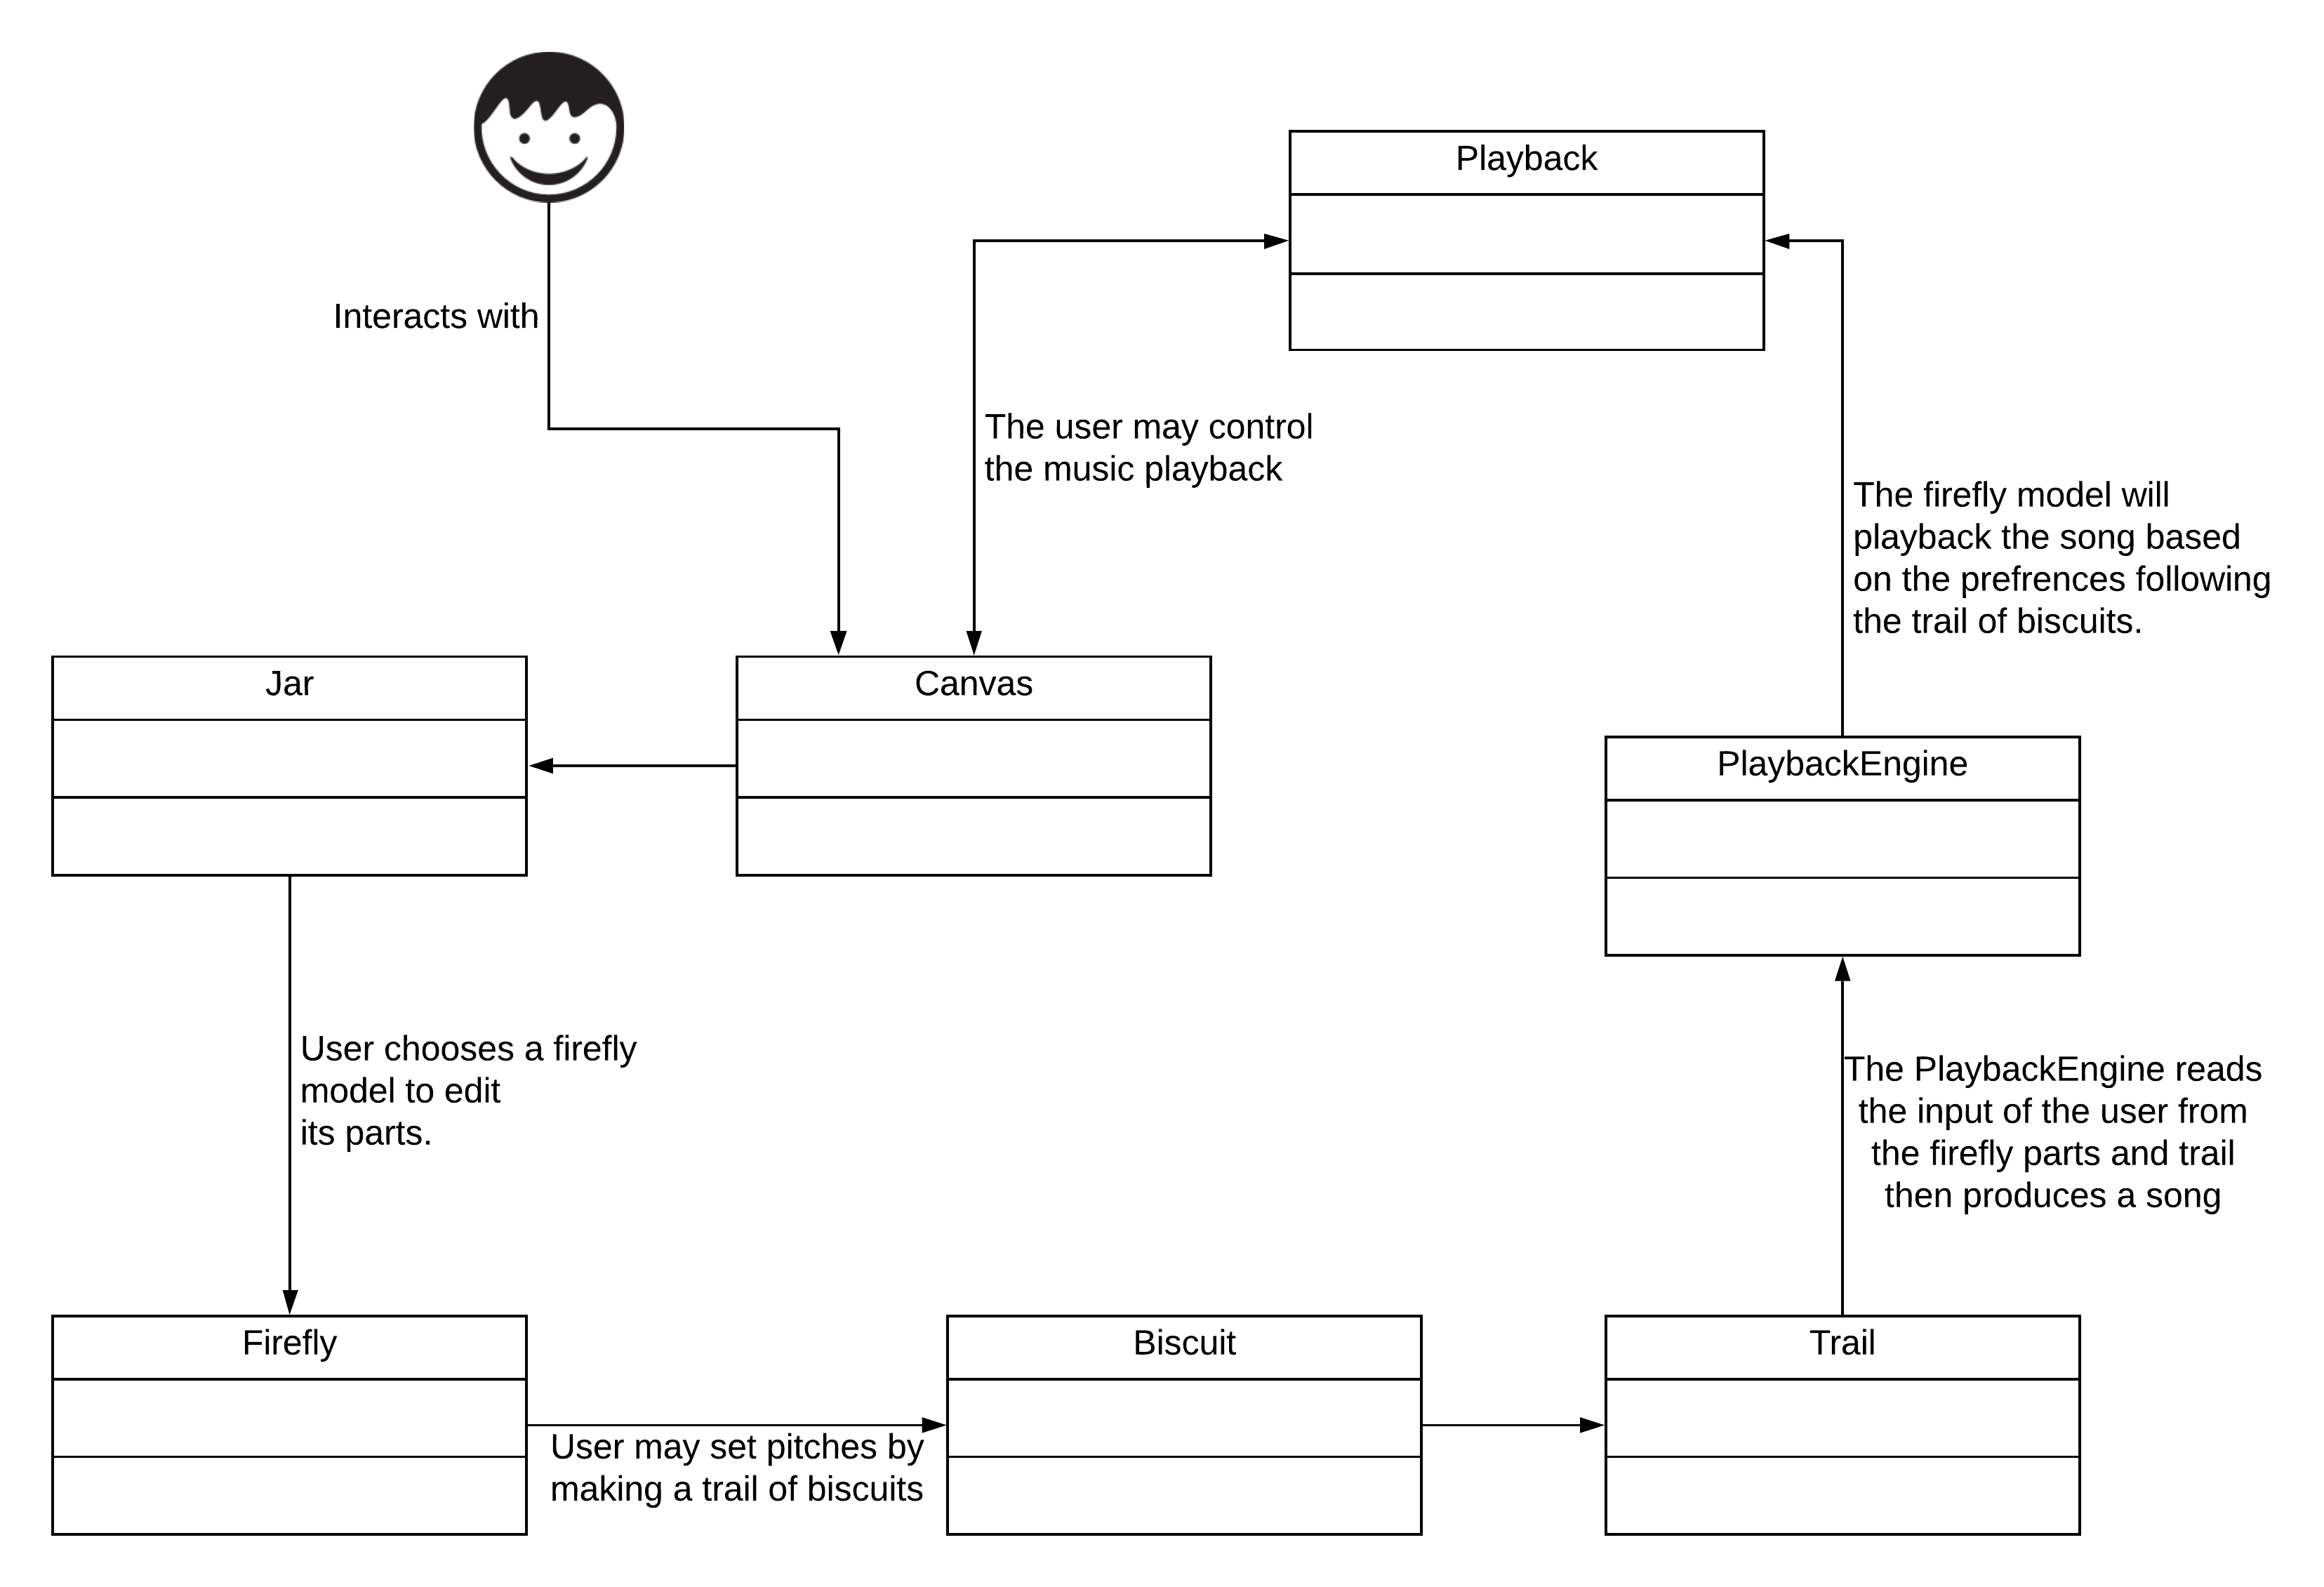
\includegraphics[width=15cm]{figures/NewSysArchi.png}
    \caption{The System Architecture of FireflyX}
    \label{fig:sysarchi}
\end{figure}

\begin{figure} [H]
    \centering
    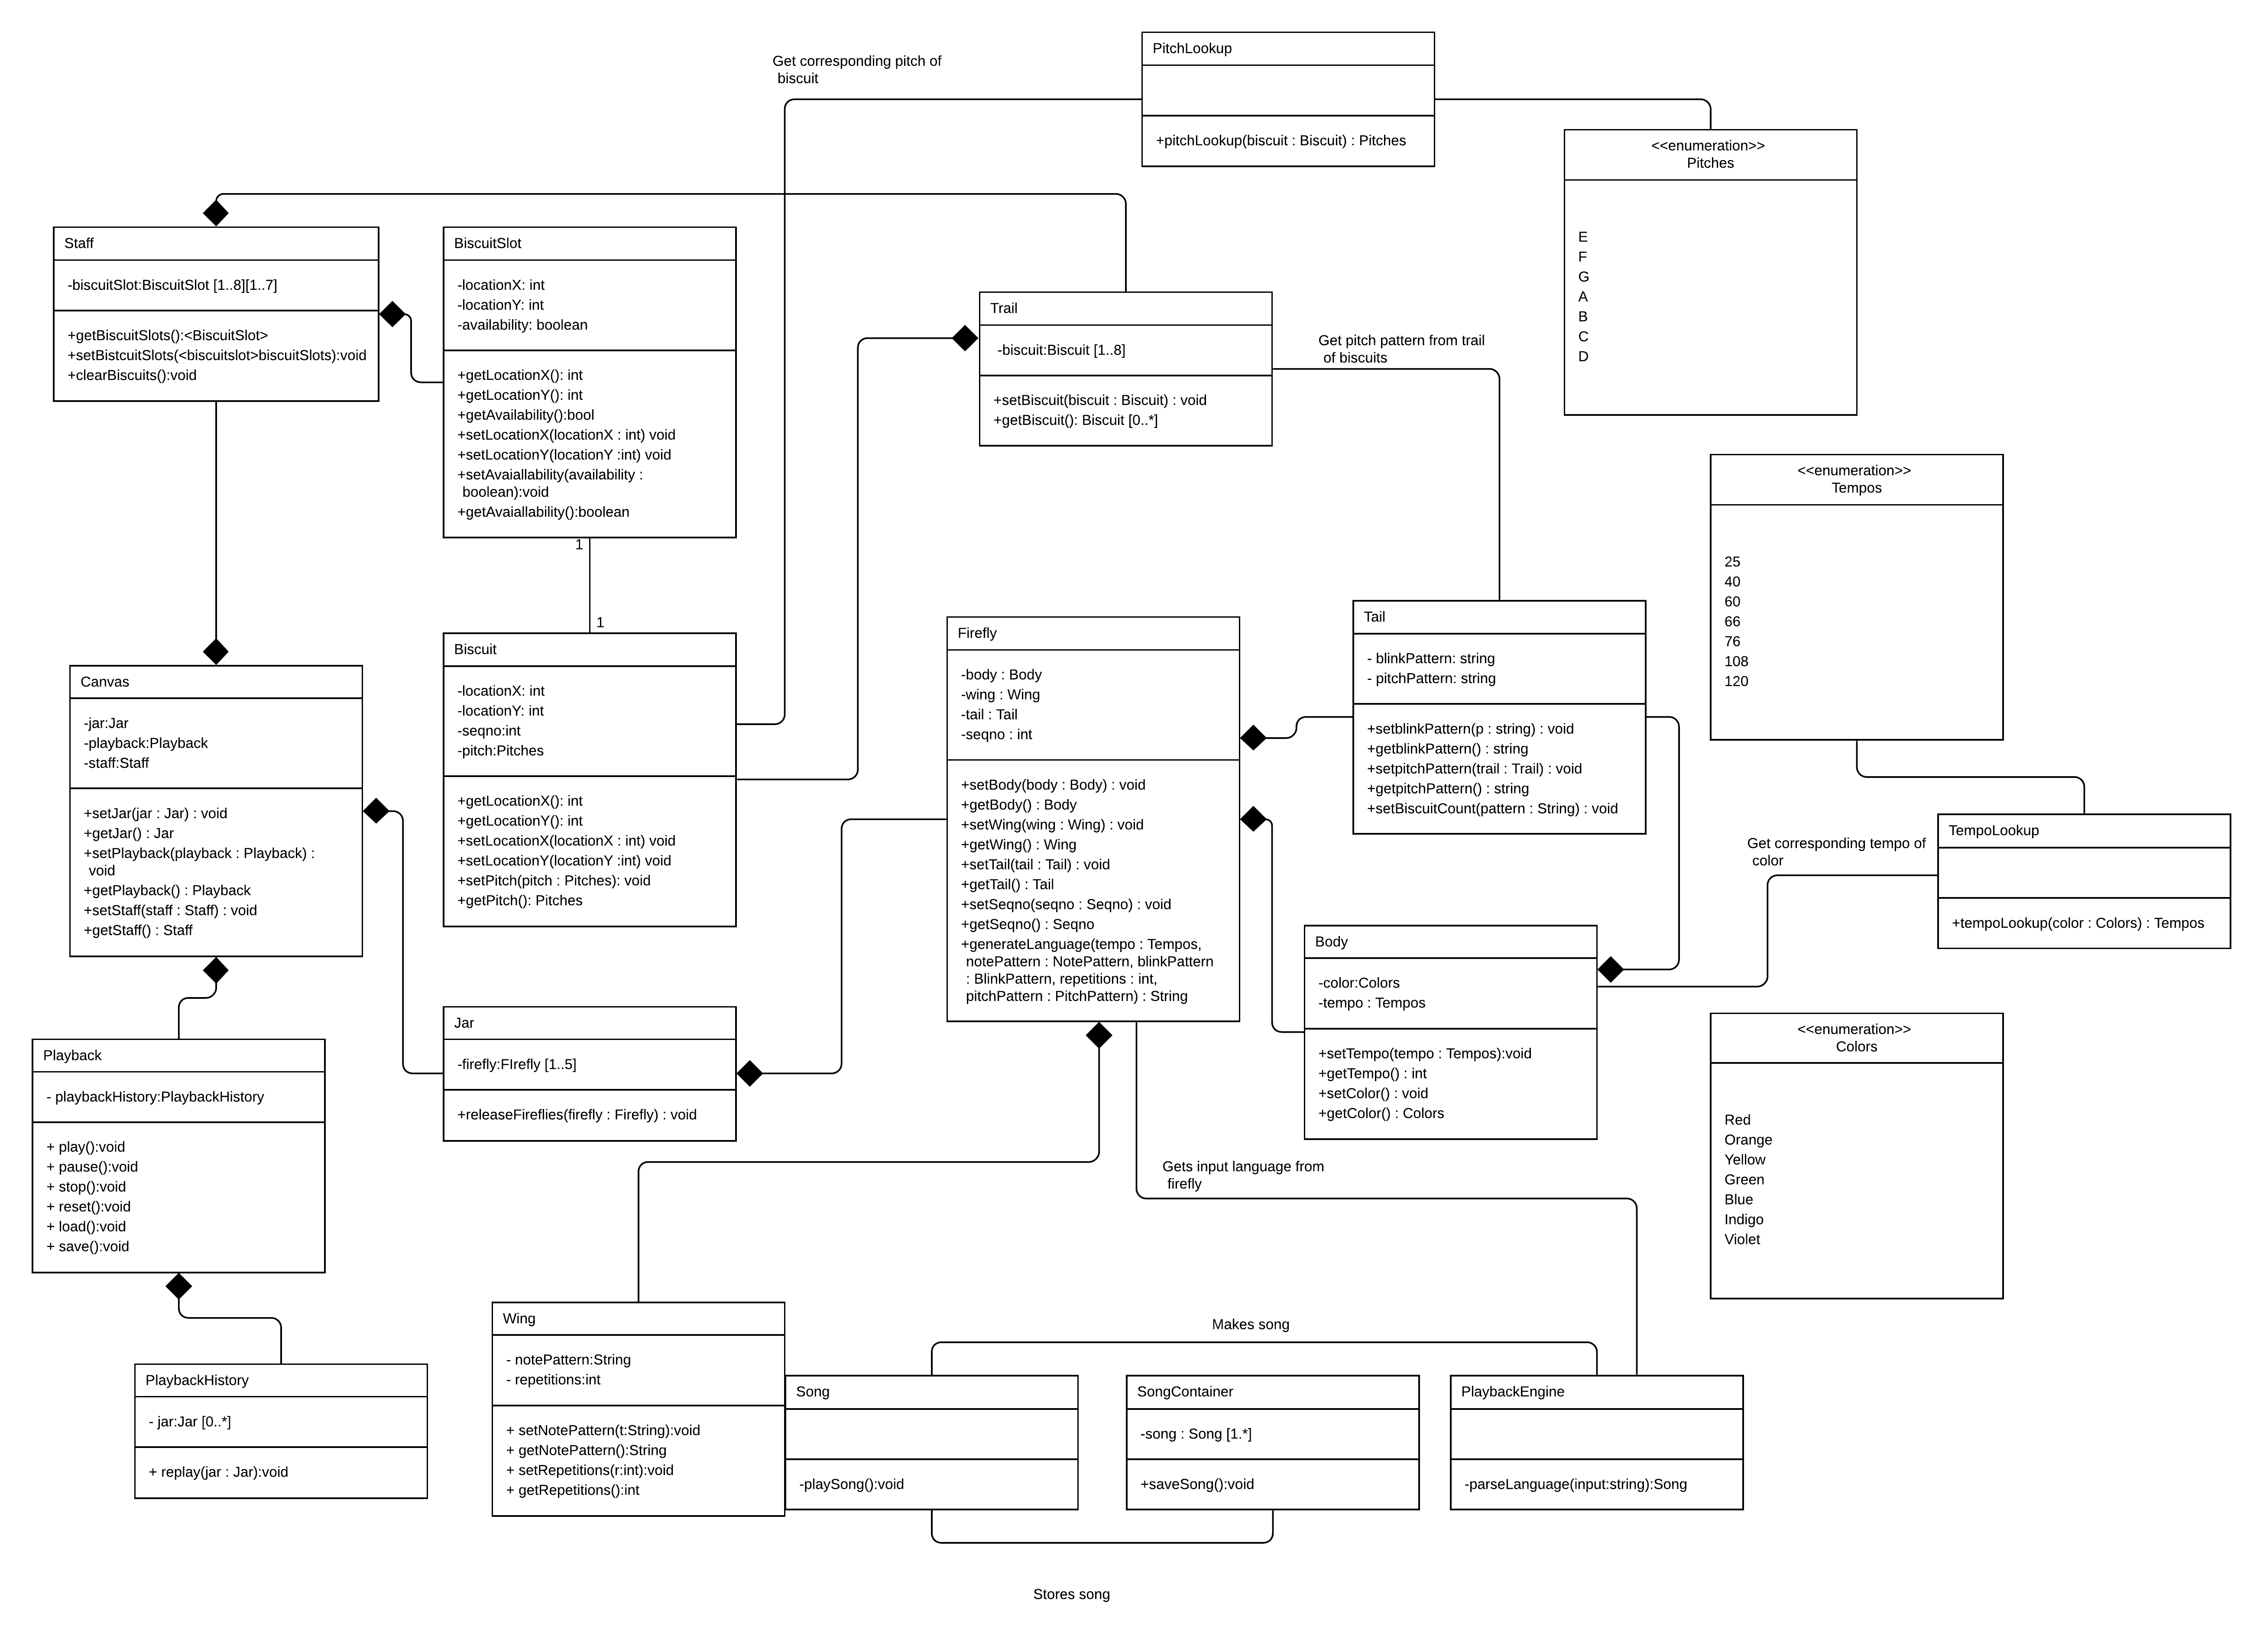
\includegraphics[width=17cm]{figures/FireflyXUML.png}
    \caption{UML Class Diagram of FireflyX}
    \label{fig:fireflyxUML}
\end{figure}

Figure \ref{fig:sysarchi} and Figure \ref{fig:fireflyxUML} shows the architecture of the system. The system follows a Model-View-Controller architecture. All processes will be handled locally by the device. Figure \ref{fig:fireflyxUML} shows the detailed class diagrams for the system.
    
\section{System Features}
The following are the features of the FireflyX application. Features such as firefly model parts popup settings, playback toolbox, jar sandbox environment, and the canvas.

% \subsection{Firefly Parts Toolbox}
% The toolbox serves to give the user the parts needed to make the firefly. The toolbox includes the head, body, wings, and the tails. Assembling different fireflies have different musical properties. These properties can be fine tuned using this toolbox. The chosen parts will correspond to a string of rhythm pattern language that will be parsed by our playback module when the firefly is released to the sandbox environment.

\subsubsection{Body Popup Settings}
The body section of the firefly model can be tapped to show the popup settings. In the popup settings of the body section, the user is able to choose the tempo of the taps that the firefly will play. Each unique color of the body has an equivalent tempo. The user can also scroll through a variety of body models. The preferences of the body will be appended to the string of rhythm pattern language. For every environment once a body has been set for the first firefly the succeeding fireflies will have the same color with the first and by changing one the others get changed as well.

\subsubsection{Wings Popup Settings}
The wing section of the firefly model can be tapped to show the popup settings. In the popup settings of the wings section, the user is able to choose the speed of the note being played by pressing 1, 2, 4, or 8 which represents the whole note, half note, quarter note, eighth note, respectively. The size of the wing will represent the number of repetitions. The minimum size is 1 and the maximum size is 6. The wing preferences will be appended to the string of rhythm pattern language.

\subsubsection{Tail Light Popup Settings}
The tail section of the firefly model can be tapped to show the popup settings. On the right side, the user is able to change the rest pattern of the note being played. The tail lights will be blinking patterns and pattern can be previewed in popup settings, the light will be based from the chosen color in the body. The patterns will be predetermined by our library of patterns. The left side will be a button for setting the pitch. The chosen pattern will be appended to the string of rhythm and pitch pattern language.

\subsubsection{Set Pitch Mode}
The mode is only accessible upon tapping the feed me button. The feed me button can be accessed during the tail pop settings. There will be a staff where the biscuits may be placed. The biscuits will be representing the notes. The number of biscuits will depend on the number of claps in the chosen pattern. The placement of the notes will also be determining the flight pattern of the firefly model. The preview button will also act like a playback for one specific firefly. The clear button will allow the user to reset the biscuits. The chosen pitch pattern will be appended to a separated pattern language.

\subsection{Jar Sandbox Environment}
The sandbox environment will be represented by a jar. In the jar, five firefly models can be seen where each can be tapped. When a firefly model is tapped, it enlarges and enables the popup settings when a specific part is tapped. The cork can also be tapped to release all of the firefly models into the canvas.

\subsection{Canvas}
Once the jar lid is tapped, the finished firefly models are released into the canvas where they roam around and play music based on their settings by sequence. Once the firefly models on the canvas are done playing they will be automatically be added to the album track list.

\subsection{Playback Control}
This toolbox will allow the user to control the playback of the firefly models. The user may pause, play, stop, and mute the music playback at anytime by clicking the play, pause, stop, and mute icons in the toolbox. The user is also able to save the existing workspace, and load a saved workspace. This can be done by clicking the save, and load buttons respectively. The user is also able to view previous tracks. In order to see the previous tracks, there will be a track list at the playback toolbox. The volume of the playback can be controlled by the slider on top of the canvas. Sliding to the sun means higher volume, and sliding to the moon means lower volume.


\section{Music Language, Rules and Library of Patterns}

\begin{table}[H]
\caption{Rhythm Representation}
\label{musiclang}
\centering
\begin{tabular}{|l|l|r|} 
\hline
Note Representation & Music Notation & Integer Equivalent  \\ 
\hline
W                   & Whole Note     & 1                   \\ 
\hline
H                   & Half Note      & 2                   \\ 
\hline
Q                   & Quarter Note   & 4                   \\ 
\hline
E                   & Eighth Note    & 8                   \\ 
\hline
Wr                  & Whole Rest     & -1                  \\ 
\hline
Hr                  & Half Rest      & -2                  \\ 
\hline
Qr                  & Quarter Rest   & -4                  \\ 
\hline
Er                  & Eighth Rest    & -8                  \\
\hline
\end{tabular}
\end{table}

\begin{table}[H]
\caption{Pitch Representation}
\label{pitchRep}
\centering
\begin{tabular}{|l|l|r|} 
\hline
Pitch of Note & Pitch Representation   \\ 
\hline
A                   & (a)                     \\ 
\hline
B                   & (b)                      \\ 
\hline
C                   & (c)                      \\ 
\hline
D                   & (d)                    \\ 
\hline
E                   & (e)                      \\ 
\hline
F                   & (f)                       \\ 
\hline
G                   & (g)                    \\ 
\hline
Rest                   & (-)                    \\ 
\hline
\end{tabular}
\end{table}

\begin{table}[H]
\caption{Tempo Representation}
\label{pitchRep}
\centering
\begin{tabular}{|l|l|r|} 
\hline
Name of Tempo & Beats Per Minute   \\ 
\hline
Grave                  & 25 bpm                     \\ 
\hline
Largo                  & 40 bpm                      \\ 
\hline
Larghetto                  & 60 bpm                      \\ 
\hline
Adagio                  & 66 bpm                    \\ 
\hline
Andante                   & 76 bpm                      \\ 
\hline
Moderato                   & 108 bpm                       \\ 
\hline
Allegro                  & 120 bpm                    \\ 
\hline
\end{tabular}
\end{table}

To help us better understand the music sheets from the Book 1 of the Suzuki teaching method, we decided to convert the sheets to a language we can easily understand and represent on code. See Table \ref{musiclang} for reference to the converted language. This will mainly be used for the representation for the first iteration since at this iteration it only covers rhythm. To make the app easier to use, a set of rules for the music composition has been used. The firefly will only be using a maximum of 6 measures per rhythm. Each measure is equal to 1 pattern. The speed of the notes and rests that will be supported by the application will only be the whole, half, quarter, and eighth note.

The following patterns are taken from the Book 1 of the Suzuki teaching method, included here are the 3 most common clap and rest patterns found in each clap and rest combination (see Table \ref{Patterns}). For the representation in the table, 1 is for the clap and the 0 is for the rest. An example as seen from the table is "1Rest" - the number 1 coefficient represents the number of instances of the rest. A change in pattern from rest to tap is separated by a dash. 

For iteration two and three since pitch will already be added we would use the same set of patterns and add a corresponding pitch to a note denoted inside a parenthesis from the seven pitches found in Table \ref{pitchRep} and also how to represent ones from a rest. An example pattern is shown through two sample pieces of music (found in Appendix \ref{sec:appendixe}), the sample representation is seen in Table \ref{PitchPatterns}.

\begin{landscape}
\begin{table}
\centering
\caption{Common Patterns in Suzuki Book 1}
\label{Patterns}
\begin{tabular}{|l|l|l|l|} 
\hline
 \textbf{Pattern}                                                                                                                                                              & \textbf{Pattern Name}                                                                                                                                                                                                    & \textbf{Count}                                                                                                                                                  & \textbf{Pattern Note Count}                                                                                                                                                                                                                \\ 
\hline
\begin{tabular}[c]{@{}l@{}}0 \\\\1\end{tabular}                                                                              & \begin{tabular}[c]{@{}l@{}}1Rest \\\\1Clap\end{tabular}                                                                                                                & \begin{tabular}[c]{@{}l@{}}23\\\\1\end{tabular}                                                               & \begin{tabular}[c]{@{}l@{}}{[}Wr - 23] \\\\{[}W - 1]\end{tabular}                                                                                                                        \\ 
\hline
\begin{tabular}[c]{@{}l@{}}001\\ \\ 010\\ \\ 100\end{tabular}              & \begin{tabular}[c]{@{}l@{}}2Rest-1Clap\\ \\ 1Rest-1Clap-1Rest\\ \\ 1Clap-2Rest \end{tabular}                         & \begin{tabular}[c]{@{}l@{}}12\\ \\ 6\\ \\ 2 \end{tabular}   & \begin{tabular}[c]{@{}l@{}}HrQrQ - 12]\\ \\ {[}QrQHr - 5, HrQQr - 1]\\ \\ {[}QQrHr - 2] \end{tabular}                                  \\ 
\hline
\begin{tabular}[c]{@{}l@{}}1010\\ \\ 1111\\ \\ 1110 \end{tabular}          & \begin{tabular}[c]{@{}l@{}}1Clap-1Rest-1Clap-1Rest\\ \\ 4Clap\\ \\ 3Clap-1Rest \end{tabular}                         & \begin{tabular}[c]{@{}l@{}}39\\ \\ 22\\ \\ 5 \end{tabular}  & \begin{tabular}[c]{@{}l@{}}QQrQQr - 39] \\ \\ {[}QQQQ - 21, EEQH - 1]\\ \\ {[}QQQQr - 5] \end{tabular}                                 \\ 
\hline
\begin{tabular}[c]{@{}l@{}}10110\\ \\ 11111\\ \\ 01101 \end{tabular}       & \begin{tabular}[c]{@{}l@{}}1Clap-1Rest-2Clap-1Rest\\ \\ 5Clap\\ \\ 1Rest-2Clap-1Rest-1Clap \end{tabular}             & \begin{tabular}[c]{@{}l@{}}26\\ \\ 10\\ \\ 13 \end{tabular} & \begin{tabular}[c]{@{}l@{}}QQrEEQr - 26]\\ \\ {[}QEEQQ -4, QQQEE -3, EQEQQ- 1, EEQQQ -1, EQQQE -1]\\ \\ {[}QrEEQrQ -13] \end{tabular}  \\ 
\hline
\begin{tabular}[c]{@{}l@{}}110110\\ \\ 111111\\ \\ 011011 \end{tabular}    & \begin{tabular}[c]{@{}l@{}}2Clap-1Rest-2Clap-1Rest\\ \\ 6Clap\\ \\ 1Rest-2Clap-1Rest-2Clap \end{tabular}             & \begin{tabular}[c]{@{}l@{}}20\\ \\ 3\\ \\ 6 \end{tabular}   & \begin{tabular}[c]{@{}l@{}} EEQrEEQr - 20 ]\\ \\ {[} EEQEEQ - 2, QQEQQE - 1 ]\\ \\ {[} QrEEQrEE - 6 ] \end{tabular}                    \\ 
\hline
\begin{tabular}[c]{@{}l@{}}1111111\\ \\ 0101011\\ \\ 0111011~\end{tabular} & \begin{tabular}[c]{@{}l@{}}7Clap\\ \\ 1Rest-1Clap-1Rest-1Clap-1Rest-2Clap\\ \\ 1Rest-3Clap-1Rest-2Clap \end{tabular} & \begin{tabular}[c]{@{}l@{}}14\\ \\ 4\\ \\ 2 \end{tabular}   & \begin{tabular}[c]{@{}l@{}} EEEEEEQ - 11, EEQEEEE - 3 ]\\ \\ {[} ErEErEErEQ - 4 ]\\ \\ {[} ErEEEErEQ - 2 ] \end{tabular}               \\ 
\hline
\begin{tabular}[c]{@{}l@{}}11110110\\ \\ 11111111 \end{tabular}                                                              & \begin{tabular}[c]{@{}l@{}}4Clap-1Rest-2Clap-1Rest\\ \\ 8Clap \end{tabular}                                                                                            & \begin{tabular}[c]{@{}l@{}}4\\ \\ 3 \end{tabular}                                                             & \begin{tabular}[c]{@{}l@{}}EEEEErEEEr - 4 ]\\ \\ {[}EEEEEEEE - 3 ] \end{tabular}                                                                                                         \\
\hline
\end{tabular}
\end{table}
\end{landscape}

\begin{table}
\centering
\caption{Patterns Found in Hot Cross Buns and Old Macdonald}
\label{PitchPatterns}
\begin{tabular}{|l|l|l|l|} 
\hline
 \textbf{Pattern }                                                                                     & \textbf{Pattern Name}                                                                                          & \textbf{Count}                                                                                   & \textbf{Pattern Note Count (with Pitch)}                                                                                                         \\ 
\hline
0                                                                                                      & 1Rest                                                                                                          & 1                                                                                                & {[}Wr(-) - 1]                                                                                                                                    \\ 
\hline
10                                                                                                     & 1Clap-1Rest                                                                                                    & 1                                                                                                & {[}H(g)Hr(-) - 1]                                                                                                                                \\ 
\hline
111                                                                                                    & 3Clap                                                                                                          & 3                                                                                                & {[}Q(b)Q(a)H(g) - 3]                                                                                                                             \\ 
\hline
\begin{tabular}[c]{@{}l@{}}1110\\\\1111\end{tabular} & \begin{tabular}[c]{@{}l@{}}3Clap-1Rest\\\\4Clap\end{tabular} & \begin{tabular}[c]{@{}l@{}}1\\\\1\end{tabular} & \begin{tabular}[c]{@{}l@{}}{[}Q(g)Q(g)Q(g)Qr(-) - 1]\\\\{[}Q(b)Q(b)Q(a)Q(a) - 1]\end{tabular}  \\ 
\hline
11111111                                                                                               & 8Clap                                                                                                          & 1                                                                                                & {[}E(b)E(b)E(b)E(b)E(a)E(a)E(a)E(a)]                                                                                                             \\
\hline
\end{tabular}
\end{table}

\section{Data Design}
Each selection of the firefly body part corresponds to an integer that references into a music library to get the necessary music files needed for the playback. The chosen format for the save files will be using XML. The file will be saving all the configurations of the current fireflies on the canvas. The file can be loaded and it will load the fireflies with their configurations that were saved on the file. The saved files will be stored locally on the device. Allowed inputs for the files can be seen in the table below in Table 5.6. An example xml file is also shown in Table \ref{XML} that shows how the sample piece Hot Cross Buns seen in Appendix \ref{sec:appendixe} will be saved.

% \begin{figure}[H]
%     \centering
%     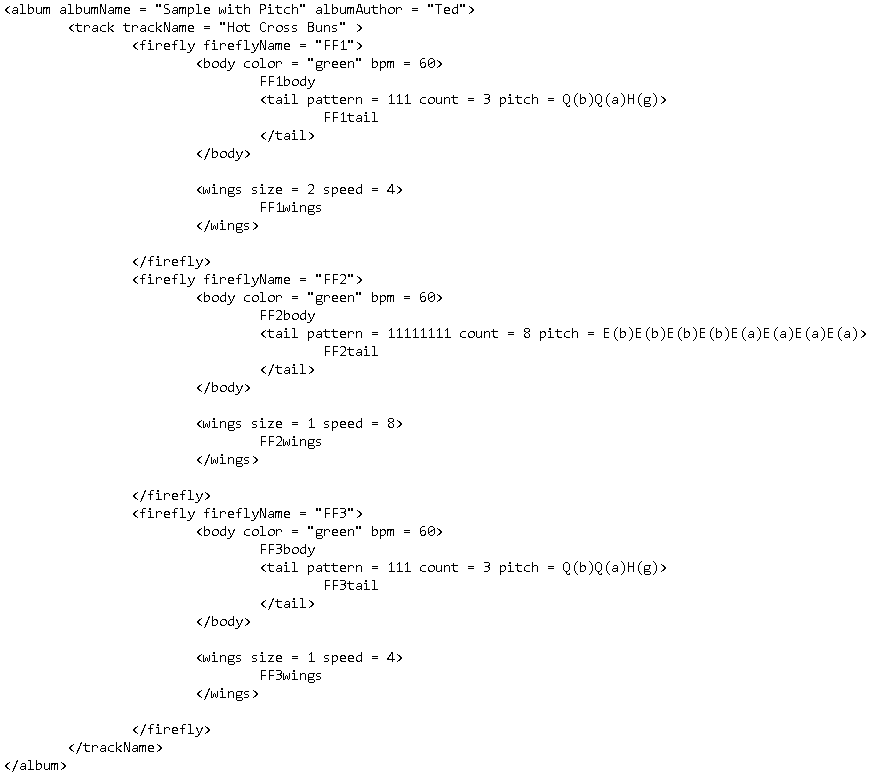
\includegraphics[width=17.6cm]{figures/sampleXML.png}
%     \caption{Sample XML}
%     \label{sampleXML}
% \end{figure}

\begin{landscape}
\begin{table}
\centering
\caption{Data Design Specifics}
\label{XML}
\begin{tabular}{|l|} 
\hline
\begin{tabular}[c]{@{}l@{}}\textless{}album albumName = "Sample with Pitch" albumAuthor = "Ted"\textgreater{}	albAlbum1						\\~ ~ ~ ~ \textless{}track trackName = "Hot Cross Buns" \textgreater{}	trkTrack1					\\~ ~ ~ ~ ~ ~ ~ ~ \textless{}firefly fireflyName = "ffObj1"\textgreater{}					\\~ ~ ~ ~ ~ ~ ~ ~ ~ ~ ~ ~ \textless{}body color = "green" bpm = 60\textgreater{}	ffObj1Body			\\~ ~ ~ ~ ~ ~ ~ ~ ~ ~ ~ ~ ~ ~ ~ ~ \textless{}tail pattern = 111 count = 3 pitch = Q(b)Q(a)H(g)\textgreater{}	ffObj1Tail		\\~ ~ ~ ~ ~ ~ ~ ~ ~ ~ ~ ~ ~ ~ ~ ~ \textless{}/tail\textgreater{}			\\~ ~ ~ ~ ~ ~ ~ ~ ~ ~ ~ ~ \textless{}/body\textgreater{}				\\~ ~ ~ ~ ~ ~ ~ ~ ~ ~ ~ ~ \textless{}wings size = 2 speed = 4\textgreater{}	ffObj1Wings			\\~ ~ ~ ~ ~ ~ ~ ~ ~ ~ ~ ~ \textless{}/wings\textgreater{}\\~ ~ ~ ~ ~ ~ ~ ~ \textless{}/firefly\textgreater{}					\\~ ~ ~ ~ ~ ~ ~ ~ \textless{}firefly fireflyName = "ffObj2"\textgreater{}					\\~ ~ ~ ~ ~ ~ ~ ~ ~ ~ ~ ~ \textless{}body color = "green" bpm = 60\textgreater{}	ffObj2Body			\\~ ~ ~ ~ ~ ~ ~ ~ ~ ~ ~ ~ ~ ~ ~ ~ \textless{}tail pattern = 11111111 count = 8 pitch = E(b)E(b)E(b)E(b)E(a)E(a)E(a)E(a)\textgreater{}	ffObj2Tail		\\~ ~ ~ ~ ~ ~ ~ ~ ~ ~ ~ ~ ~ ~ ~ ~ \textless{}/tail\textgreater{}			\\~ ~ ~ ~ ~ ~ ~ ~ ~ ~ ~ ~ \textless{}/body\textgreater{}				\\~ ~ ~ ~ ~ ~ ~ ~ ~ ~ ~ ~ \textless{}wings size = 1 speed = 8\textgreater{}	ffObj2Wings			\\~ ~ ~ ~ ~ ~ ~ ~ ~ ~ ~ ~ \textless{}/wings\textgreater{}\\~ ~ ~ ~ ~ ~ ~ ~ ~\textless{}/firefly\textgreater{}					\\~ ~ ~ ~ ~ ~ ~ ~ ~\textless{}firefly fireflyName = "ffObj3"\textgreater{}					\\~ ~ ~ ~ ~ ~ ~ ~ ~ ~ ~ ~ \textless{}body color = "green" bpm = 60\textgreater{}	ffObj3Body			\\~ ~ ~ ~ ~ ~ ~ ~ ~ ~ ~ ~ ~ ~ ~ ~ \textless{}tail pattern = 111 count = 3 pitch = Q(b)Q(a)H(g)\textgreater{}	ffObj3Tail		\\~ ~ ~ ~ ~ ~ ~ ~ ~ ~ ~ ~ ~ ~ ~ ~ \textless{}/tail\textgreater{}			\\~ ~ ~ ~ ~ ~ ~ ~ ~ ~ ~ ~ \textless{}/body\textgreater{}				\\~ ~ ~ ~ ~ ~ ~ ~ ~ ~ ~ ~ \textless{}wings size = 1 speed = 4\textgreater{}	ffObj3Wings~ \\~ ~ ~ ~ ~ ~ ~ ~ ~ ~ ~ ~ \textless{}/wings\textgreater{}\\~ ~ ~ ~ ~ ~ ~ ~ \textless{}/firefly\textgreater{}	\\~ ~ ~ ~ \textless{}/trackName\textgreater{}						\\\textless{}/album\textgreater{}	\end{tabular}  \\
\hline
\end{tabular}
\end{table}
\end{landscape}

% \begin{landscape}
% \begin{table}[]
% \label{XML}
% \caption{Data Design Specifics}
% \begin{tabular}{|l|l|l|l|}
% \hline
% Tags                            & Possible inputs              & Description                                                                                                                                                               & Correspondence \\ \hline
% \textless{}album\textgreater{}       & varchar     & \begin{tabular}[c]{@{}l@{}}The album will contain the author, \\ \\ album name, and tracks.\end{tabular}                                                                  & 1-*            \\ \hline
% \textless{}track\textgreater{}       & fireflies                    & \begin{tabular}[c]{@{}l@{}}There will be a maximum of 5 fireflies per\\ track.\end{tabular}                                                                               & 1-*            \\ \hline
% \textless{}firefly\textgreater{}     & body, wings, and tail light  & \begin{tabular}[c]{@{}l@{}}The firefly represents a rhythm that the\\ user defined by assembling their firefly.\end{tabular}                                              & 1-*            \\ \hline
% \textless{}body\textgreater{}        & sequence and instrument      & \begin{tabular}[c]{@{}l@{}}The body represents the sequence and\\ instrument of the rhythm.\end{tabular}                                                                  & 1-*            \\ \hline
% \textless{}sequence\textgreater{}    & 1,2,3,4,5                    & \begin{tabular}[c]{@{}l@{}}Represents the order of playback in the canvas. \\ \\ 1 means its the first firefly to run, 3, means 3rd.\end{tabular}                         & 1-1            \\ \hline
% \textless{}instrument\textgreater{}  & Guitar, Piano, Violin, Drum, & Represents the instrument to be played back.                                                                                                                              & 1-1            \\ \hline
% \textless{}wings\textgreater{}       & speed and size               & \begin{tabular}[c]{@{}l@{}}The wings represent the speed\\ and repetitions of the rhythm.\end{tabular}                                                                    & 1-*            \\ \hline
% \textless{}speed\textgreater{}       & 1,2,4,8                      & \begin{tabular}[c]{@{}l@{}}Represents the seed of the note. 1 means\\ \\ whole note, 2 means half note, \\ \\ 4 means quarter note, and 8 means eighth note.\end{tabular} & 1-1            \\ \hline
% \textless{}size\textgreater{}        & 1,2,3,4,5,6                  & \begin{tabular}[c]{@{}l@{}}Represents the number\\ of repetition of the firefly.\end{tabular}                                                                             & 1-1            \\ \hline
% \textless{}taillight\textgreater{}   & Rest pattern and color       & \begin{tabular}[c]{@{}l@{}}Represents the rest pattern and color\\ of the rhythm.\end{tabular}                                                                            & 1-*            \\ \hline
% \textless{}restpattern\textgreater{} & Check library of patterns    & \begin{tabular}[c]{@{}l@{}}Represents the clap rest\\ pattern of the firefly. Example is \\ 1010 which means clap - rest - clap - rest\end{tabular}                       & 1-1            \\ \hline
% \textless{}color\textgreater{}       & Hex-code of colors            & \begin{tabular}[c]{@{}l@{}}Represents the color emitted by the tail light of\\ the firefly. Example is \#FFFFFF means white.\end{tabular}                                 & 1-1            \\ \hline
% \end{tabular}
% \end{table}
% \end{landscape}

\begin{landscape}
\begin{table}
\centering
\caption{Data Design Specifics}
\label{XML}
\begin{tabular}{|p{2cm}|p{2.8cm}|p{6.6cm}|p{9cm}|} 
\hline
 \textbf{Tag}                    & \textbf{Attribute}                                                                      & \textbf{Possible Values}                                                                                                        & \textbf{Description}                                                                                                                                                                                                                                                                                                                                                                                                      \\ 
\hline
\textless{}album \textgreater{}  & \begin{tabular}[c]{@{}l@{}}albumName\\{}authorName \end{tabular} & \begin{tabular}[c]{@{}l@{}}varchar=Album1\\{}string=Ted \end{tabular}                    & The album will contain the author and album name it will also include tracks.                                                                                                                                                                                                                                                                                                                                             \\ 
\hline
\textless{}track\textgreater{}   & trackName                                                                               & varchar=Track 1                                                                                                 & There will be a maximum of 5 fireflies per track.                                                                                                                                                                                                                                                                                                                                                                         \\ 
\hline
\textless{}firefly\textgreater{} & fireflyName                                                                             & varchar=ffObj1                                                                                                     & The firefly represents the rhythm and pitch that the user has defined by assembling their firefly                                                                                                                                                                                                                                                      \\ 
\hline
\textless{}body\textgreater{}    & \begin{tabular}[c]{@{}l@{}}color\\{}bpm \end{tabular}            & \begin{tabular}[c]{@{}l@{}}color=Red\\{}integer=25 \end{tabular}                                          & The body represents the tempo of the firefly. The colors are limited to the seven colors of the rainbow to represent the 7 pitches.                                                                                                                                                                                     \\ 
\hline
\textless{}wings\textgreater{}   & \begin{tabular}[c]{@{}l@{}}size\\{}speed \end{tabular}           & \begin{tabular}[c]{@{}l@{}}integer=5\\{}integer=8 \end{tabular}                                            & The wings represent the speed and repetitions of the rhythm. The values of size are limited from 1-6 and the speed are values representing the speed of the notes from slowest to fastest 1,2,4,8.                                                                                           \\ 
\hline
\textless{}tail\textgreater{}    &   
\begin{tabular}[c]{@{}l@{}}pattern\\{}count\\{}pitch \end{tabular}     


& \begin{tabular}[c]{@{}l@{}}integer=1010 \\{}integer=4\\{}string=Q(f)Qr(-)Q(a)Qr(-) \end{tabular} & Represents the clap rest pattern and color based on the tempo of the body. Example is 1010 which means 1Clap-1Rest-1Clap-1Rest with a count of 4. The pitch pattern on the~other hand is also retrieved for the making of the biscuits that represent the different pitches.  \\
\hline
\end{tabular}
\end{table}
\end{landscape}

\section{Screen Flows}

% All use cases can be seen in Appendix \ref{sec:appendixb}.

\subsection{Splash Screen}

\begin{figure}[H]
    \centering
    
\includegraphics[width=10cm]{figures/Splash.png}
    \caption{Splash Screen}
    \label{fig:splash}
\end{figure}

The Splash Screen is the first screen shown to the child when the application is opened. The splash screen will last for 3 seconds.

\subsection{Main Menu}

\begin{figure}[H]
    \centering
    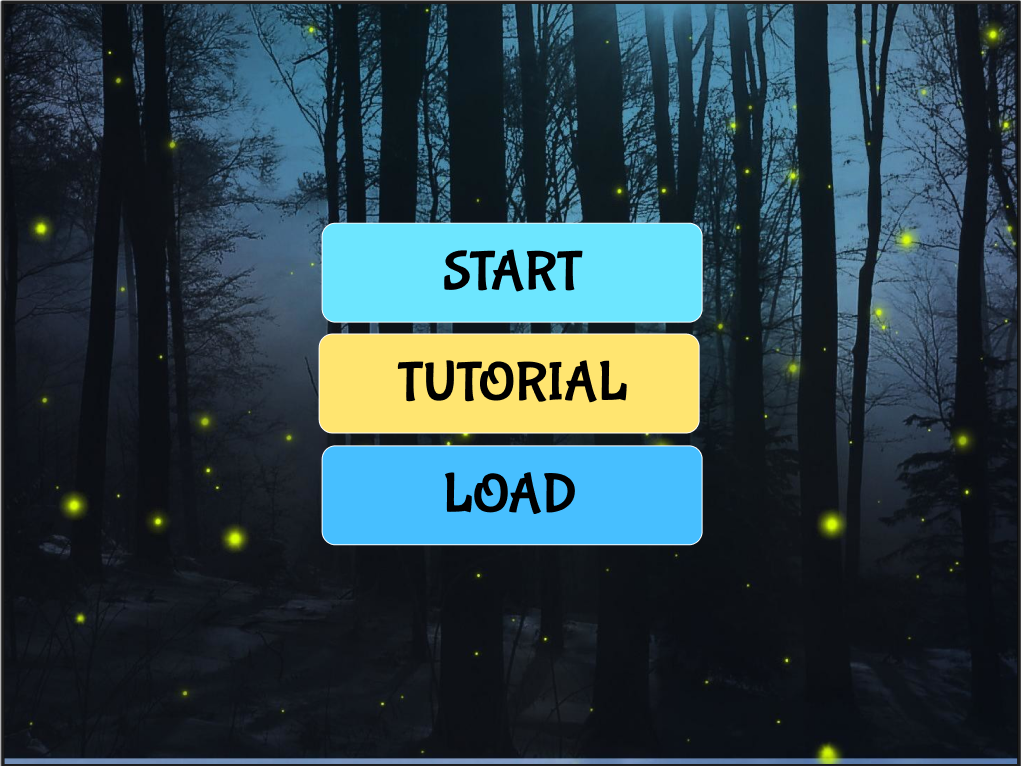
\includegraphics[width=10cm]{figures/MainMenu.png}
    \caption{Main Menu}
    \label{fig:mainmenu}
\end{figure}

The Main Menu (figure \ref{fig:mainmenu}) is the next screen that will show after the splash screen, here the child may tap between 3 buttons, namely: start, tutorial, and load. The start button will open a blank workspace. The tutorial button will show the user how to assemble the firefly step by step and the different gestures that will be utilized. The load button will open the Load Menu where the user may load saved workspaces.

\subsection{Start New}

\begin{figure}[H]
    \centering
    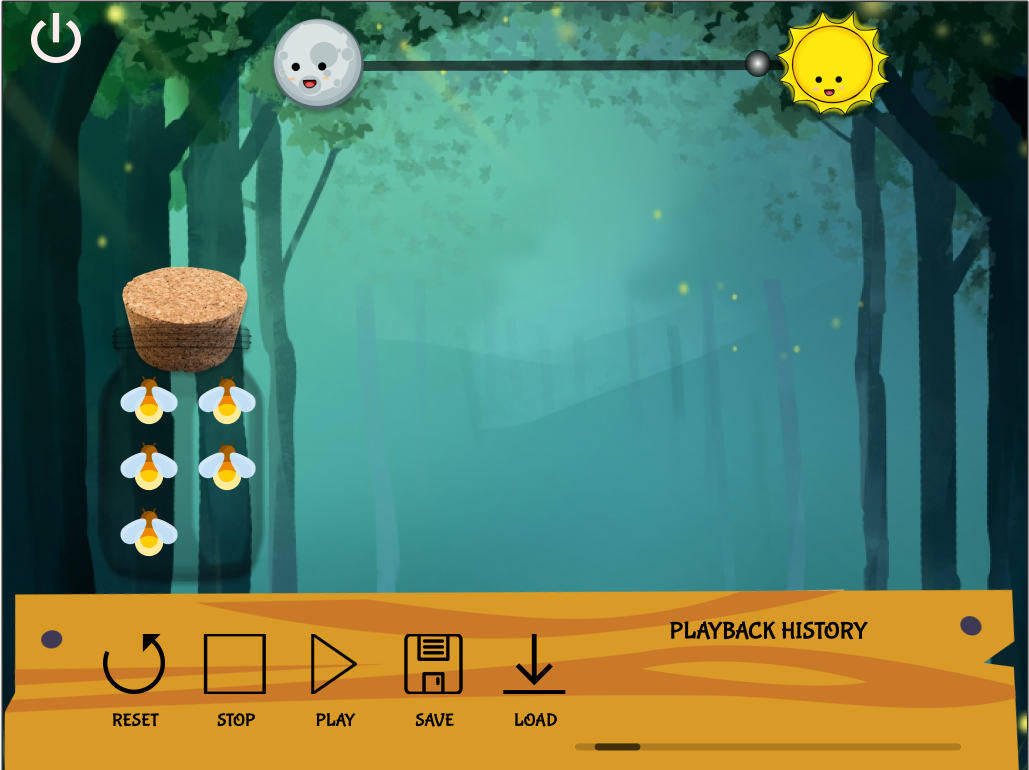
\includegraphics[width=10cm]{figures/BlankSpace.png}
    \caption{Blank Workspace}
    \label{fig:blankworkspace}
\end{figure}

After tapping Start button this is the blank workspace that the child will see figure \ref{fig:blankworkspace}. In this screen, the user will see a jar of fireflies, and other playback controls. This screen is important as this follows the principle of an Obvious Starting point as it becomes a starting point in the application that the child can first explore different interactions and also a safe space for the child as they know that if they commit something wrong they can always go back to this screen.

\subsection{Edit Firefly}

\begin{figure}[H]
    \centering
    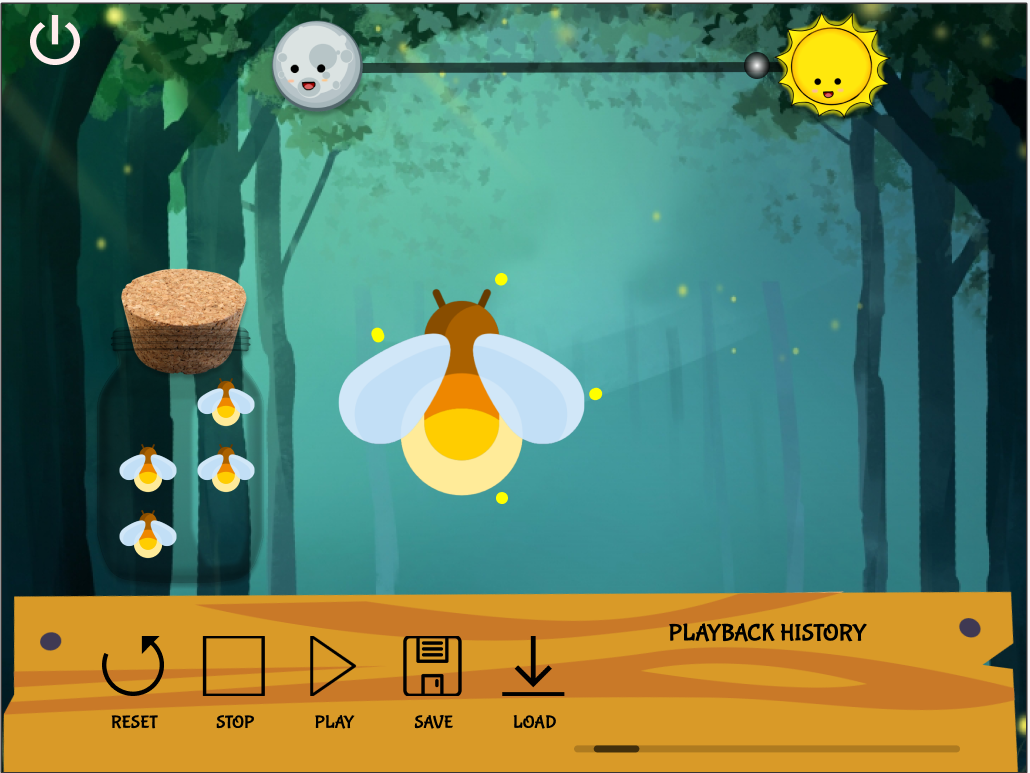
\includegraphics[width=10cm]{figures/ChooseFirefly.png}
    \caption{Editing a Firefly}
    \label{fig:editfirefly}
\end{figure}

After Loading a blank workspace, the child may choose a firefly model to edit by tapping any of the small fireflies in the jar. After tapping a firefly model in the jar, the firefly model will be enlarged so that the child may tap a firefly part to edit. We decided to use simple tap gestures for tasks involved in manipulating the firefly parts to make it easier for the child to remember them and to reduce the load of the actions that can be caused by using other gestures.  

\subsection{Edit Firefly Body}

\begin{figure}[H]
    \centering
    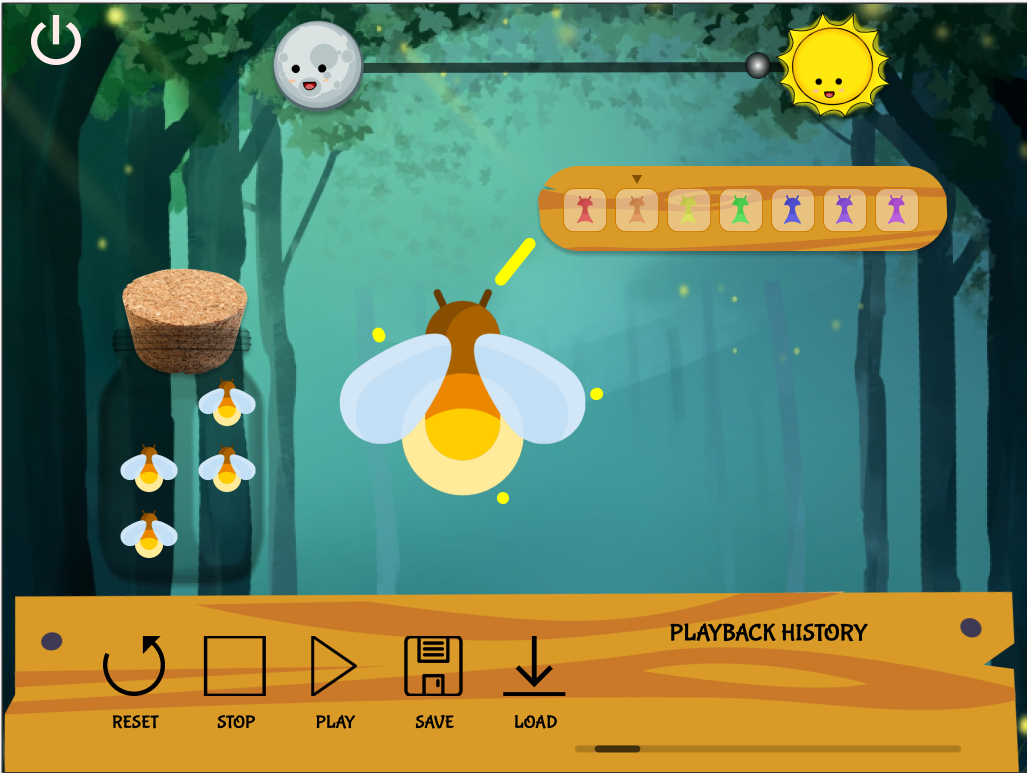
\includegraphics[width=10cm]{figures/Body.png}
    \caption{Editing Firefly Body}
    \label{fig:tweakBody}
\end{figure}

After choosing a firefly model to edit, the child may tap the body to show the popup settings that can configure the properties. The different body color corresponds to different tempos.

\subsection{Edit Firefly Wing}

\begin{figure}[H]
    \centering
    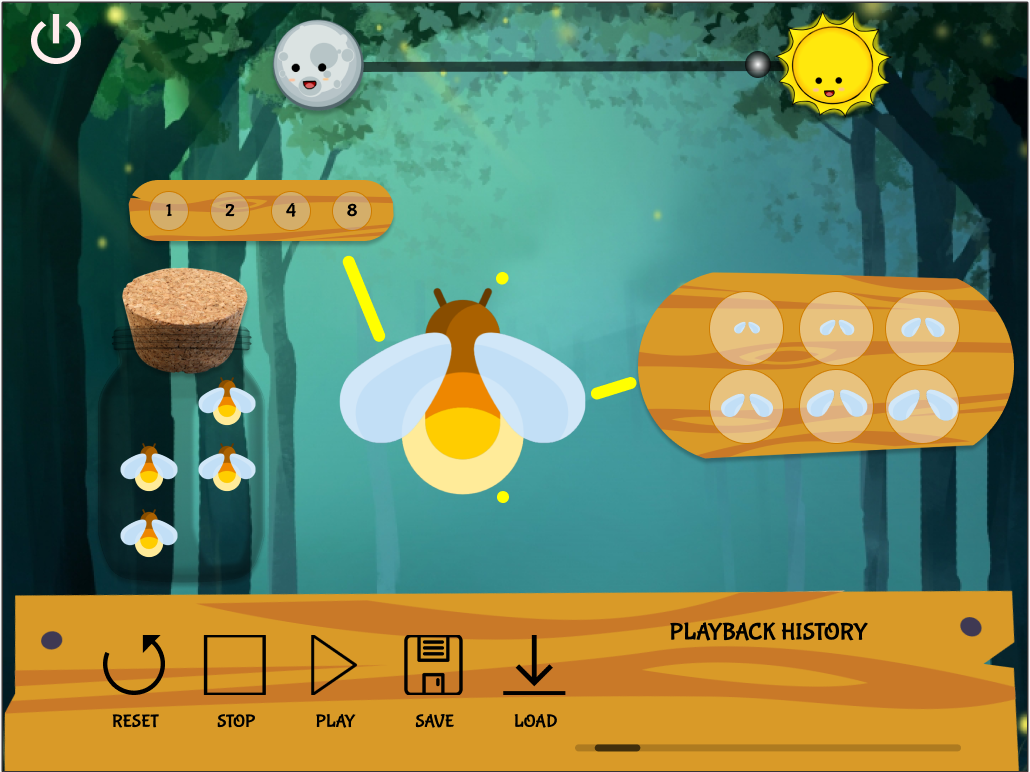
\includegraphics[width=10cm]{figures/Wing.png}
    \caption{Editing Firefly Wing}
    \label{fig:tweakWing}
\end{figure}

After choosing a firefly model to edit, the child may tap the wing to show the popup settings that can configure the properties. For the wing popup settings, there will be two bubbles. The first bubble is for configuring the wing speed. The different wing speed corresponds to length of notes. The other wing configures the wing size. The different wing size corresponds to different number of repetitions. 

\subsection{Edit Firefly Tail Light}

\begin{figure}[H]
    \centering
    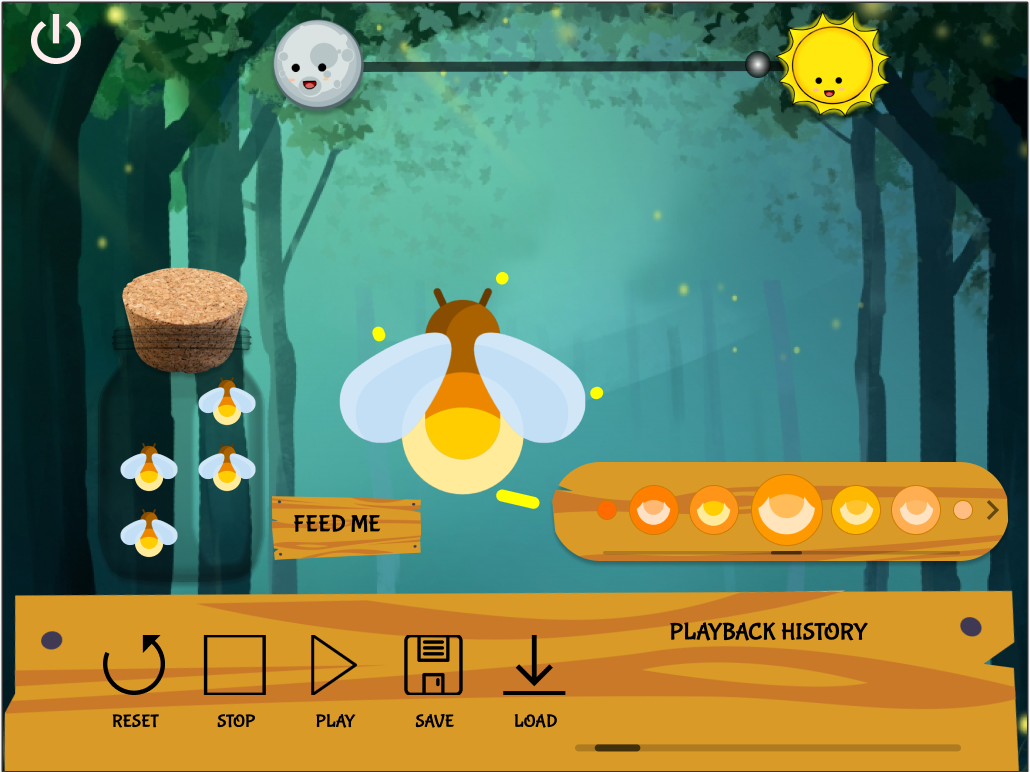
\includegraphics[width=10cm]{figures/Tail.png}
    \caption{Editing Firefly Tail Light}
    \label{fig:tweakTail}
\end{figure}

After choosing a firefly model to edit, the child may tap the tail light to show the popup settings that can configure the properties.

\subsection{Feed Firefly}

\begin{figure}[H]
    \centering
    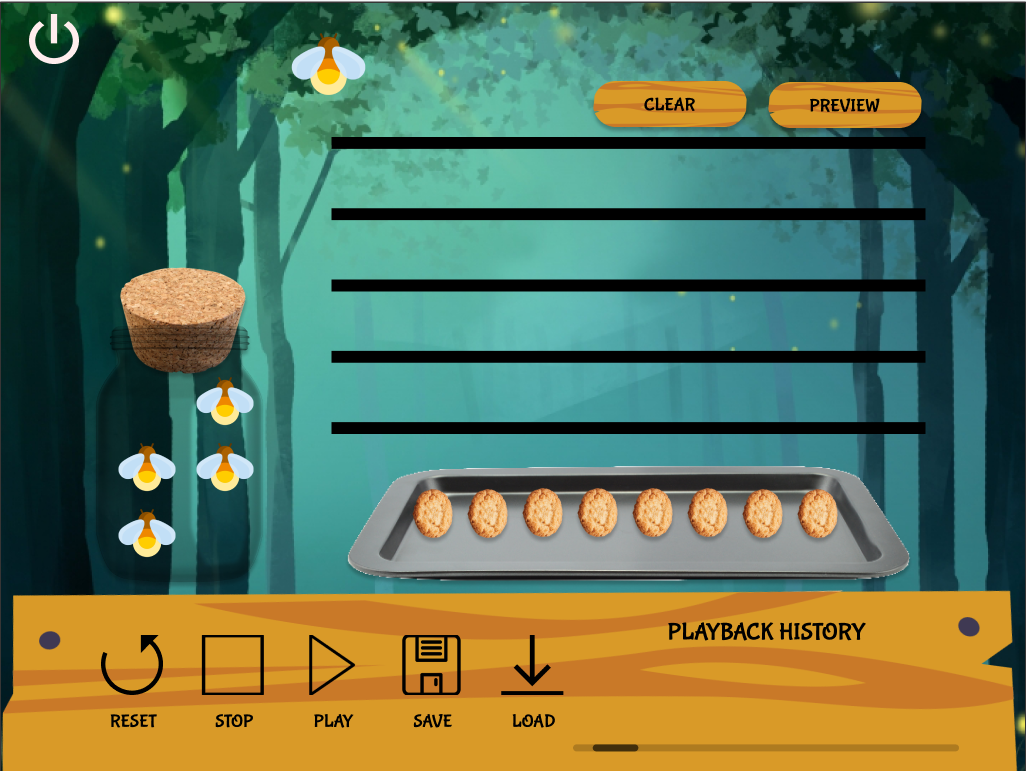
\includegraphics[width=10cm]{figures/FeedFirefly.png}
    \caption{Set Pitch of Notes by Feeding the Firefly}
    \label{fig:feedfirefly}
\end{figure}

After choosing the preferred tail light, the user may tap the feed me button in order to set the biscuits for the path of the firefly model which will also determine the pitch of the notes that the firefly model will play.

\begin{figure}[H]
    \centering
    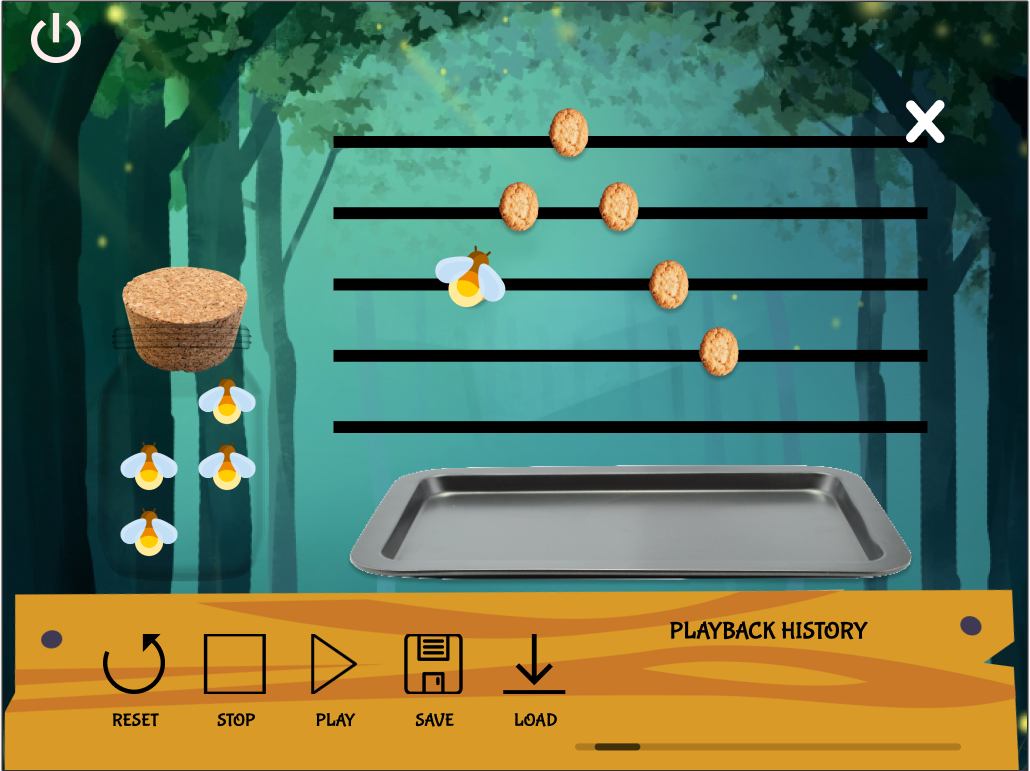
\includegraphics[width=10cm]{figures/PreviewEatingTrail.png}
    \caption{Preview Flight Pattern}
    \label{fig:previewFLight}
\end{figure}

The user may also see a preview of how the firefly model will fly based on their placed biscuits by tapping the preview button.

\subsection{Change Currently editing firefly}

\begin{figure}[H]
    \centering
    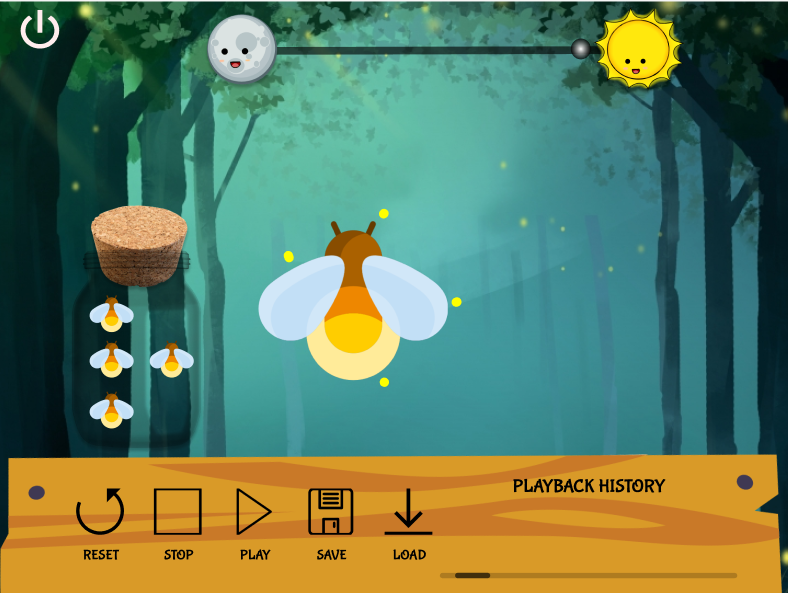
\includegraphics[width=10cm]{figures/ChangeFirefly.png}
    \caption{Choosing Different Firefly to Edit}
    \label{fig:firefly2}
\end{figure}

In order to change the currently editing firefly model to a different firefly model. The child can simply click any of the smaller fireflies to enlarge and the previously enlarged firefly model will minimize. We wanted this action to show a contrast of sizes so that the child focus will shift from the one currently made to the new one.

\subsection{Release Fireflies to start playback}

\begin{figure}[H]
    \centering
    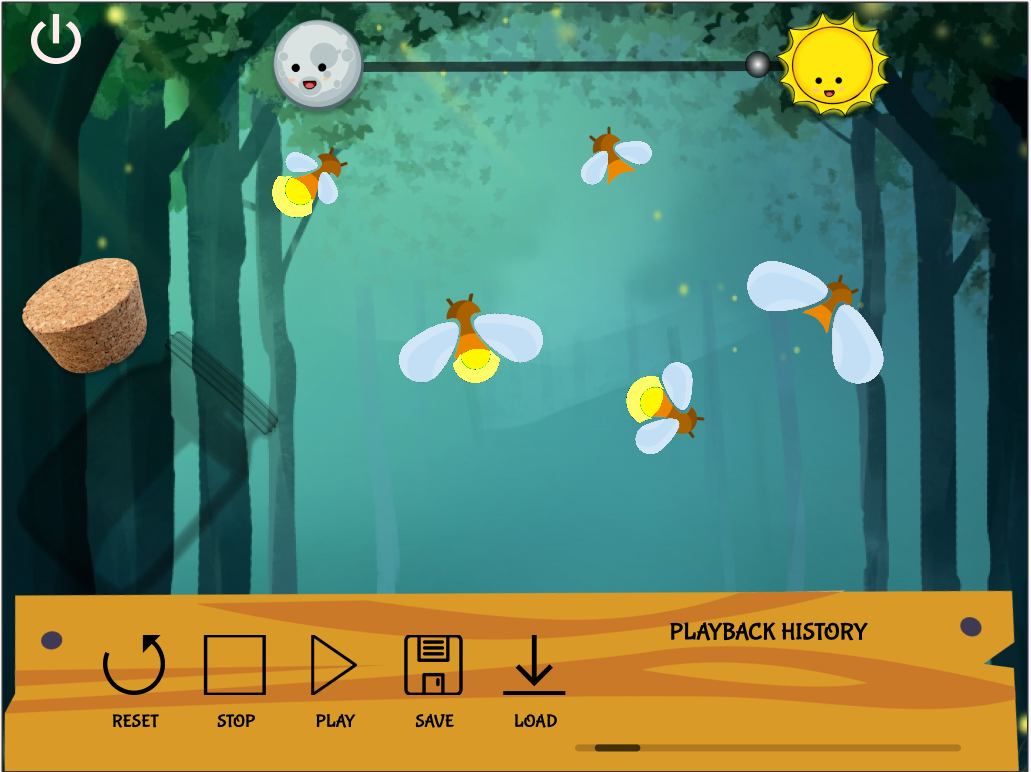
\includegraphics[width=10cm]{figures/Release.png}
    \caption{Releasing the Fireflies}
    \label{fig:releaseFirefly}
\end{figure}

After editing the firefly models to desired configurations, the child can tap on the lid of the jar to release all the fireflies and start the rhythm playback. This particular action was chosen as the start of the playback since we wanted it to represent the real world where fireflies are released and the child can see it as a way of familiarity.

\subsection{Pause, Play, and Stop playback}

\begin{figure}[H]
    \centering
    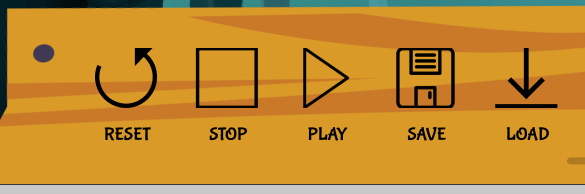
\includegraphics[width=6cm]{figures/StopPlayPause.png}
    \caption{Play Pause, and Stop Controls}
    \label{fig:firefly2}
\end{figure}

During playback, the child can pause and play the playback by toggling the play button. The stop button stops the current playback and starts the playback from the start on pause. The design of the buttons was made to be familiar buttons as they can already give the child an idea of what the buttons do.
 
\subsection{Adjusting Volume}

\begin{figure}[H]
    \centering
    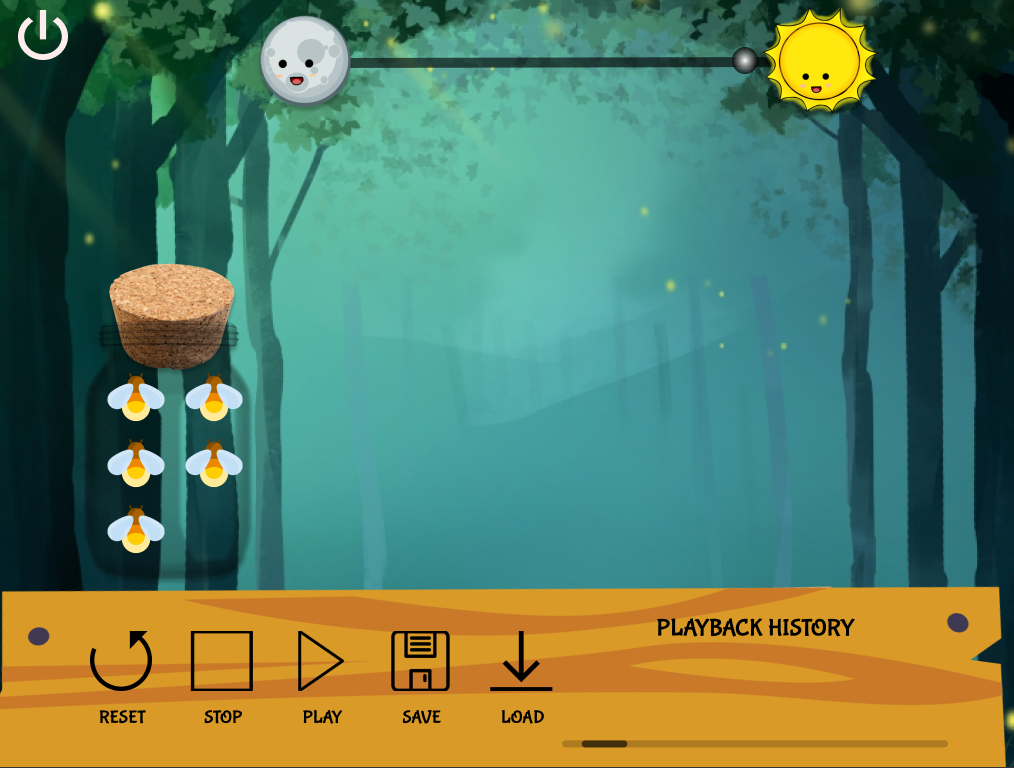
\includegraphics[width=6cm]{figures/volumecontrol.png}
    \caption{Changing Volume of Playback}
    \label{fig:volcontrol}
\end{figure}

During playback, the child can adjust the volume of the playback by using the slider between the sun and moon. The moon will represent a lower volume and the sun will represent a higher volume. One finger drag gesture will be used as the child has more control of the desired volume they need with the use of this gesture.

\subsection{Replay Previous Tracks}

\begin{figure}[H]
    \centering
    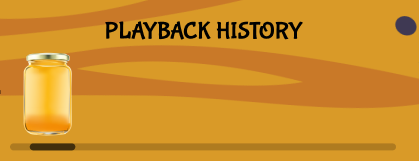
\includegraphics[width=6cm]{figures/historyplayback.png}
    \caption{List of Previous Tracks}
    \label{fig:firefly2}
\end{figure}

After the firefly models are done with their playback, they are placed on to the playback history. The user may play these previous tracks again by dragging them to the jar on the left side then press play. This also was designed to represent the real world action of catching and releasing a firefly.

\subsection{Reset Album}

\begin{figure}[H]
    \centering
    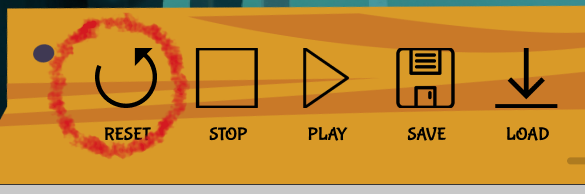
\includegraphics[width=6cm]{figures/resetwork.png}
    \caption{Reset Album Button}
    \label{fig:firefly2}
\end{figure}

If the child wishes to start fresh with a new blank album, the child may press the reset button to return everything to default. We needed to put this as the child can go back to the start which is a screen where he is already familiar with and he would know there is a way to undo their mistakes.

\subsection{Save Album}

\begin{figure}[H]
    \centering
    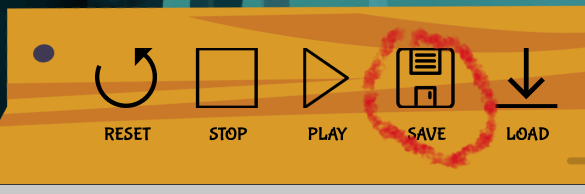
\includegraphics[width=6cm]{figures/Save.png}
    \caption{Save Album Button}
    \label{fig:firefly2}
\end{figure}
The child may choose to save the existing album at anytime. Upon tapping the save button, the child is asked to input an author name and a title for the album. After confirming the album is then saved to the local device and can be loaded at anytime.
\subsection{Load Album}

\begin{figure}[H]
    \centering
    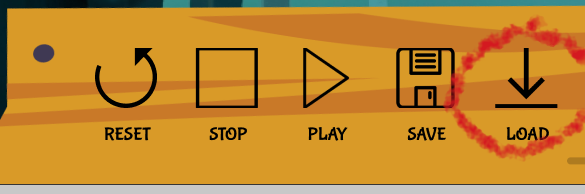
\includegraphics[width=6cm]{figures/load.png}
    \caption{Load Album Button}
    \label{fig:firefly2}
\end{figure}

The child may choose to load an existing album at anytime by tapping the load button.

\subsection{Load Menu}

\begin{figure}[H]
    \centering
    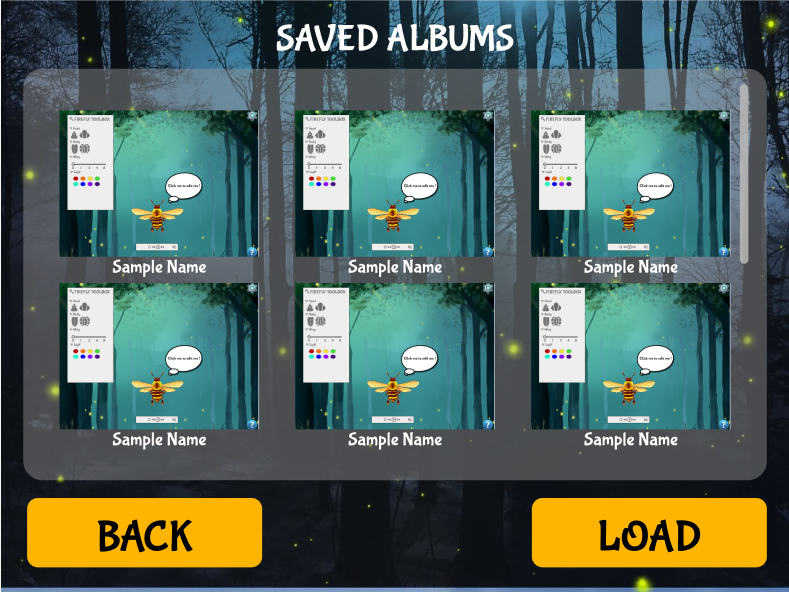
\includegraphics[width=6cm]{figures/LoadMenu.png}
    \caption{Load Menu}
    \label{fig:loadmenu}
\end{figure}

The Load Menu shows all saved albums/workspaces. The child may tap on an album then press the load button to continue working on that album.

\subsection{Exit to Main Menu}

\begin{figure}[H]
    \centering
    \includegraphics[width=6cm]{figures/exitmenu.png}
    \caption{Exit Button}
    \label{fig:exitbutton}
\end{figure}

The child may choose to tap the exit to main button at any time. When the button is pressed, a confirmation appears and when the child confirms that they want to exit to main menu, the screen will be transferred to the main menu. Same as the start screen this will give the child a sense of relief knowing they can go back to the start and begin all over again.
% \section{Use Case Diagram}
% \begin{figure}[!htb]
%     \centering
%     \includegraphics{figures/UseCaseDiagram.PNG}
%     \caption{Use Case Diagram of Firefly}
%     \label{fig:my_label}
% \end{figure}

% This is the use case diagram of Firefly. These are all the actions that the user is allowed to do within the application.

\section{Deployment Plan}
FireflyX will be developed using Xcode using the Swift language. The application once compiled can be uploaded to the Apple App Store where anyone may download the app for free but with in-game purchases. The files will be saved locally this includes the songs and the environment, these files will be exportable with the use of the XML. Using the XML another user in a different iPad can retrieve the same environment by loading the XML sent. A diagram showing the deployment plan is shown in figure \ref{deploymentPlan}.

\begin{figure}[H]
    \centering
    \includegraphics[width=15cm]{figures/deploymentPlan.png}
    \caption{FireflyX Deployment Plan}
    \label{deploymentPlan}
\end{figure}                 %-- includes LaTeX source file for Chapter 5: System Design

%%%%%%%%%%%%%%%%%%%%%%%%%%%%%%%%%%%%%%%%%%%%%%%%%%%%%%%%%%%%%%%%%%%%%%%%%%%%%%%%%%%%%%%%%%%%%%%%%%%%%%
%
%   Filename    : chapter_6.tex 
%
%   Description : This file will contain your Preliminary Results.
%                 
%%%%%%%%%%%%%%%%%%%%%%%%%%%%%%%%%%%%%%%%%%%%%%%%%%%%%%%%%%%%%%%%%%%%%%%%%%%%%%%%%%%%%%%%%%%%%%%%%%%%%%
\chapter{Preliminary Results}
\section{Demographic of Respondents}
Interviewees were gathered by going to music schools and asking if the music teachers were fine being interviewed. We were able to interview 5 music teachers from different music schools. As a prerequisite, they are required to have at least 5 years of experience in teaching music by the time they participate. The demographic of the characteristics of these music teachers are shown in Table \ref{Demographics}.

\begin{table}
\label{Demographics}
\centering
\caption{Demographic Characteristics of Music Teachers}
\begin{tabular}{|l|l|} 
\hline
Characteristic  & Total(n=5)    \\ 
\hline
Age (mean \pm   SD [range]) & 39.8 \pm    14.5 [22-57]              \\ 
\hline
\begin{tabular}[c]{@{}l@{}}Sex (n [\%])\\~~~ Male\\~~~ Female\end{tabular}                                                 & \begin{tabular}[c]{@{}l@{}} 4 [80]\\1 [20]\end{tabular}                 \\ 
\hline
Years of Experience (mean \pm   SD [range])                                                                                    & 20.6 \pm    10.4 [7-35]                                                          \\ 
\hline
\begin{tabular}[c]{@{}l@{}}Preferred Teaching Method (n [\%])\\~~~ Suzuki\\~~~ Traditional\end{tabular}                    & \begin{tabular}[c]{@{}l@{}} 3 [60]\\2 [40]\end{tabular}                  \\ 
\hline
\begin{tabular}[c]{@{}l@{}}Specialty (n [\%])\\~~~ Violin\\~~~ Piano\\~~~ Voice\\~~~ Trumpet\end{tabular}                  & \begin{tabular}[c]{@{}l@{}} 2 [40]\\1 [20]\\1 [20]\\1 [20]\end{tabular}  \\ 
\hline
\begin{tabular}[c]{@{}l@{}}Recommended Musical Fundamental to Teach (n [\%])\\~~~ Rhythm\\~~~ Pitch \& Rhythm\end{tabular} & \begin{tabular}[c]{@{}l@{}} 3 [60]\\2 [40]\end{tabular}                  \\
\hline
\end{tabular}
\end{table}

\section{Understanding Children Needs}
From the interviews of the music teachers, we were able to compile a few key points that will help us identify the needs of children.
\begin{itemize}
    \item It is important to have the children's attention before teaching anything to them.
    \item The child should also be comfortable with the teacher, in addition to this the child must also feel safe and have trust in the teacher. This will help the child in expressing themselves.
    \item There are multiple ways to get the trust of children. Some are: icebreaker, pep talk, talking to them, and asking how their day is going.
    \item The teacher should assess them to know how to teach them.
    \item The teacher should adjust to the child.
    \item Repetition with development is important. Present the same idea differently.
    \item Teacher's passion will pass on the children.
    \item Rhythm must be taught first to children. It is usually done through clapping.
    \item Every session must be interesting and the curiosity of the child must be exploited.
    \item Learning should be step-by-step. Every part must be understood completely before moving on.
    \item Suzuki method teaches discipline to children. By having discipline, the child is able to study more efficiently alone.
    \item Traditional Method is just teaching the topic to the child. It is more of a by-the-book method, and usually instructional.
\end{itemize}

From the key points that were identified, a scenario map was created as shown in figure \ref{fig:ScenarioMap}

\begin{figure}[H]
    \centering
    \includegraphics[width=16cm]{figures/ScenarioMaps.png}
    \label{fig:ScenarioMap}
    \caption{The digital version of the scenario map taking into account the key points from the interviews. Blue = Step, Yellow = Question, Green = Idea, Pink = Solution.}
\end{figure}

% Based on our interviews with the music teachers, we were able to hypothesize some features needed by children. These hypotheses were then clarified with them and verified. After these, it was then translated into features for the mid-fidelity prototype as shown in Table \ref{BasicFeatureTranslations}.
% \begin{table}[]
% \label{BasicFeatureTranslations}
% \caption{Basic Feature Translations. H = Hypothesis, C = Clarification,  V =Verification, T = Translation.}
% \begin{tabular}{|p{14cm}|}
% \hline
% \begin{tabular}[c]{@{}l@{}}\textbf{H:} Children would want to edit existing fireflies and explore other options or \\ settings. \\ \textbf{C:} Asked the music teacher if the child will edit existing fireflies.\\ \textbf{V:} Verified that the child would want to have the option to edit fireflies. This \\will allow the child to explore other combinations.\\ \textbf{T:} Added feature that allowed fireflies to be edited before released.\end{tabular} \\ \hline
% \begin{tabular}[c]{@{}l@{}}\textbf{H:} The child would want to replay previous tracks.\\ \textbf{C:} Asked the teacher if the child will replay previous tracks.\\ \textbf{V:} Verified that the child will want to replay previous tracks and listen \\again to the track. This will let the child to  have a clearer understanding on \\how the configurations affected the sound produced.\\ \textbf{T:} Added a feature that allowed replaying of previous tracks.\end{tabular} \\ \hline
% \begin{tabular}[c]{@{}l@{}}\textbf{H:} The child would want to save and load workspace.\\\textbf{C:} Asked the teacher if the child would want to save the existing workspace \\or load an existing workspace.\\ \textbf{V:} Verified that the child would want to save the existing workspace to allow \\them to exit the workspace anytime or load a workspace anytime. This will \\allow the child to have the freedom of continuing whenever they want to.\\ \textbf{T:} Added feature that allowed the saving of existing workspace, and loading \\of an existing workspace. \end{tabular} \\ \hline
% \begin{tabular}[c]{@{}l@{}}\textbf{H:} The child would want to reset the workspace and delete all configurations \\of the fireflies.\\ \textbf{C:} Asked the teacher if the child would want to reset the workspace.\\ \textbf{V:} Verified that the child would want to reset the workspace and reset all the \\configurations of the fireflies. This will allow the child to quickly get rid of all \\the configurations and start from scratch.\\ \textbf{T:} Added feature that allowed resetting the workspace and delete all the \\configurations of the fireflies.\end{tabular} \\ \hline
% \end{tabular}
% \end{table}
% \section{Mid-fidelity Prototype}
% \begin{figure}[H]
%     \centering
%     \includegraphics[width=16cm]{figures/Prototype1.png}
%     \caption{The first version of the mid-fidelity prototype built using Figma}
%     \label{fig:Prototype1}
% \end{figure}

% The mid-fidelity prototype consists of 3 spaces, namely: canvas, sandbox, and toolbox. A firefly can be built using the toolbox on the sandbox environment. The toolbox feature took inspiration from a number of applications that require drag and drop such as Lucid Chart, and Gravit. After the firefly is assembled it can be dragged on to the canvas where the firefly will roam and playback the rhythm configuration. 

% Transfer tables here in overleaf
% https://docs.google.com/document/d/1wLBHrv6spsFyLCrxCDzhwrFCYW9UCK_8IP80yTavOrM/edit
                 %-- includes LaTeX source file for Chapter 6: Preliminary Results

\bibliography{sample_bibliography}

\appendix                         %-- used to specify appendices
%%%%%%%%%%%%%%%%%%%%%%%%%%%%%%%%%%%%%%%%%%%%%%%%%%%%%%%%%%%%%%%%%%%%%%%%%%%%%%%%%%%%%%%%%%%%%%%%%%%%%%
%
%   Filename    : appendix_A.tex 
%
%   Description : This file is for including the Research Ethics Documents (delegated as Appendix A) 
%                 
%%%%%%%%%%%%%%%%%%%%%%%%%%%%%%%%%%%%%%%%%%%%%%%%%%%%%%%%%%%%%%%%%%%%%%%%%%%%%%%%%%%%%%%%%%%%%%%%%%%%%%

\chapter{Research Ethics Documents}
\label{sec:appendixa}


\begin{comment}

IMPORTANT -- READ THIS PART!!!

Please follow the instructions below on how to include the Research Ethics documents 
in your proposal document (typeset using LaTeX):

1. Open, and accomplish the contents of the THREE Word DOCX files included in the distribution

2. Once you're done filling in the necessary items, save the file in PDF format.  This is done by clicking on \say{File}, 
    then \say{Save As} and then choose PDF (not DOCX default option) .  Do this for the three documents.

   The filenames are long, so I renamed the files with shorter names: 
       a . clearance.PDF  (original was GradSchool-revised ethics clearance form)
       b. general_checklist.PDF (original was General Research Ethics Checklist)
       c.  checklist-A PDF (original was [Specific Checklists] Checklist A - Human Participants]

\end{comment}

\includepdf[pages=-, scale = 0.9, pagecommand={}, offset = -30 0]{Ethics5clearance.pdf}

\includepdf[pages=-, scale = 0.9, pagecommand={}, offset = -30 0]{Ethics1.pdf}

\includepdf[pages=-, scale = 0.9, pagecommand={}, offset = -30 0]{Ethics2CheckA.pdf}

\includepdf[pages=-, scale = 0.9, pagecommand={}, offset = -30 0]{Ethics3CheckF.pdf}

\includepdf[pages=-, scale = 0.9, pagecommand={}, offset = -30 0]{Ethics4ParentalConsent.pdf}

\includepdf[pages=-, scale = 0.9, pagecommand={}, offset = -30 0]{Ethics6TeacherConsent.pdf}



              %-- includes LaTeX source file for Appendix A
             
\chapter{Turnitin Similarity Report}
\label{sec:appendixb}

\includegraphics[width=17cm]{similarityReport.png}
%%%%%%%%%%%%%%%%%%%%%%%%%%%%%%%%%%%%%%%%%%%%%%%%%%%%%%%%%%%%%%%%%%%%%%%%%%%%%%%%%%%%%%%%%%%%%%%%%%%%%%
%
%   Filename    : appendix_B.tex
%
%   Description : This file will contain information about your Resource Persons
%                 
%%%%%%%%%%%%%%%%%%%%%%%%%%%%%%%%%%%%%%%%%%%%%%%%%%%%%%%%%%%%%%%%%%%%%%%%%%%%%%%%%%%%%%%%%%%%%%%%%%%%%%

\chapter{Use Cases}
\label{sec:appendixc}

For the headers of each row the cases that will be used are: 
\begin{itemize}
    \item Trigger - The goal that the user case is designed for
    \item Primary Actor - Main entities that are directly involved in achieving goal
    \item Supporting Actors - Additional entities that can influence achieving the goal but are not directly involved
    \item Preconditions - Conditions that need to be satisfied before the process starts
    \item Process Steps - Step by step actions the primary actor does in order to achieve the goal
    \item Minimal Guarantees - The outcome in the scenario that the goal is only partially
    \item Success Guarantees - The outcome in the scenario that the goal is fully done

\end{itemize}

%
%  Indicate your resource persons here:
%
%	<full name and title, e.g., Dr. Juan de la Cruz>
%	<profession, e.g., faculty>
%	<department, e.g., College of Computer Studies>
%	<name of institution, e.g., De La Salle University>
%	<e-mail address>
%
%

\begin{table}
\centering
\begin{tabular}{|p{5cm}|p{10.2cm}|} 
\hline
\multicolumn{2}{|l|}{\textbf{Use Case 1: Child explores the workspace in the screen}}                                                           \\ 
\hline
\textbf{Trigger}            & \begin{tabular}[c]{@{}l@{}}Upon entry on the workspace the child is curious on the \\assets found on the screen\end{tabular}                                                                                            \\ 
\hline
\textbf{Primary Actor}      & Child                                                                                                                                                                                                          \\ 
\hline
\textbf{Supporting Actors}  & \begin{tabular}[c]{@{}l@{}}• Sandbox\\• FireflyX \end{tabular}                                                                                                                                                 \\ 
\hline
\textbf{Precondition}       & \begin{tabular}[c]{@{}l@{}}• The user has already pressed start in the main menu\\• The child has finished the tutorial~ ~ ~ ~ ~ ~ ~ ~ ~ ~ ~ ~ ~ ~ ~ ~ ~ ~ ~ ~ ~ ~ ~ ~ ~ ~ ~ ~ ~ ~ ~ ~ ~ ~ ~ ~ ~\end{tabular}  \\ 
\hline
\textbf{Process Steps}      & \begin{tabular}[c]{@{}l@{}}1. The child taps on the many assets found on the screen\\2. The child selects one of the five available fireflies \\in the jar, thus activating firefly creation\end{tabular}           \\
\hline
% \hline
% \textbf{Minimal Guarantees} & \begin{tabular}[c]{@{}l@{}}The child might miss-tap and not select the \\firefly they intended to select\end{tabular}  \\ 
% \hline
% \textbf{Success Guarantees} & The correct firefly is selected                                                                                        \\
\end{tabular}
\end{table}

\begin{table}
\centering
\begin{tabular}{|p{5cm}|p{10.2cm}|} 
\hline
\multicolumn{2}{|l|}{\textbf{Use Case 2: Select tempo for the fireflies in an environment to represent }}                                                                                                                                                                                   \\ 
\hline
\textbf{Trigger}            & \begin{tabular}[c]{@{}l@{}}The child wants the firefly to have a speed of a \\ certain tempo              \end{tabular}                                                                                                                                                                 \\ 
\hline
\textbf{Primary Actor}      & Child                                                                                                                                                                                                                                          \\ 
\hline
\textbf{Supporting Actors}  & \begin{tabular}[c]{@{}l@{}}• Firefly object\\• Sandbox\\• FireflyX\end{tabular}                                                                                                                                                                       \\ 
\hline
\textbf{Precondition}       & \begin{tabular}[c]{@{}l@{}}• The user has pressed start in the main menu\\• This should be the first part that is modified in a \\specific firefly\end{tabular}                                                                                             \\ 
\hline
\textbf{Process Steps}      & \begin{tabular}[c]{@{}l@{}}1. The child taps the firefly's body\\2. The child taps the color of the tempo arranged\\from slowest to fastest in the pop up settings\\3.When the tail is selected later on it should show the \\same color selected by the child\end{tabular}  \\ 
% \hline
% \textbf{Minimal Guarantees} & \begin{tabular}[c]{@{}l@{}}An instrument is not added to the firefly in the sandbox \\environment\end{tabular}                                                                                                                                 \\ 
% % \hline
% % \textbf{Success Guarantees} & \begin{tabular}[c]{@{}l@{}}The body of the firefly will change based on the \\selected instrument\end{tabular}                                                                                                                                 \\
\hline
\end{tabular}
\end{table}

\begin{table}
\centering
\begin{tabular}{|p{5cm}|p{10.2cm}|} 
\hline
\multicolumn{2}{|l|}{ \textbf{Use Case 3: Select pitch for the each note to represent } }                                                                                                                                                                                                                                                                                                                                                 \\ 
\hline
\textbf{Trigger}            & \begin{tabular}[c]{@{}l@{}}The child wants the firefly to represent a certain \\ pitch for each note\end{tabular}                                                                                                                                                                                                                                                                   \\ 
\hline
\textbf{Primary Actor}      & Child                                                                                                                                                                                                                                                                                                                                                                                                       \\ 
\hline
\textbf{Supporting Actors}  & \begin{tabular}[c]{@{}l@{}}• Firefly object\\ • Sandbox\\ • FireflyX \end{tabular}                                                                                                                                                                                                                                                                          \\ 
\hline
\textbf{Precondition}       & \begin{tabular}[c]{@{}l@{}}• The user has pressed start in the main menu\\ • The firefly should have its parts like the wings,\\ body, and tail already configured\\ \end{tabular}                                                                                                                                                  \\ 
\hline
\textbf{Process Steps}      & \begin{tabular}[c]{@{}l@{}}1. The child taps on the firefly\\ 2. The child configures the wings, body, and tail\\ 3. The child selects Feed Me to start editing~\\ the biscuits\\ 4. The child puts the biscuits in the locations~\\ of the pitch notes in the staff\end{tabular}  \\
\hline
\end{tabular}
\end{table}

\begin{table}
\centering
\begin{tabular}{|p{5cm}|p{10.2cm}|} 
\hline
\multicolumn{2}{|l|}{\textbf{Use Case 4: Select number of repetitions of the rhythm}}                                                                                                                                                                                                                                                                                           \\ 
\hline
\textbf{Trigger}            & \begin{tabular}[c]{@{}l@{}}The child would want the a pattern to have a number \\ of repetitions\end{tabular}                                                                                                                                                                                                                              \\ 
\hline
\textbf{Primary Actor}      & Child                                                                                                                                                                                                                                                                                                                                             \\ 
\hline
\textbf{Supporting Actors}  & \begin{tabular}[c]{@{}l@{}}•Firefly object\\•Sandbox\\•FireflyX\end{tabular}                                                                                                                                                                                                                                                                             \\ 
\hline
\textbf{Precondition}       & \begin{tabular}[c]{@{}l@{}}• The user has pressed start in the main menu\\• The firefly can already have other parts already \\modified\end{tabular}                                                                                                                                                                                                \\ 
\hline
\textbf{Process Steps}      & \begin{tabular}[c]{@{}l@{}}1. The child taps the firefly's wing\\2. The child selects a wing size from the six possible in\\ the pop-up settings, where the smallest with a wing \\pattern of one would mean it will repeat only in one \\measure and the biggest with a wing pattern of six\\ where it will repeat for six measures.\end{tabular}  \\ 
% \hline
% \textbf{Minimal Guarantees} & The repetition still remains as one                                                                                                                                                                                                                                                                                                               \\ 
% \hline
% \textbf{Success Guarantees} & \begin{tabular}[c]{@{}l@{}}The body of the firefly will change based on the selected \\instrument\end{tabular}                                                                                                                                                                                                                                    \\
\hline
\end{tabular}
\end{table}

\begin{table}
\centering
\begin{tabular}{|p{5cm}|p{10.2cm}|} 
\hline
\multicolumn{2}{|l|}{\textbf{Use Case 5: Select speed of the rhythm}}                                                                                                                                                                              \\ 
\hline
\textbf{Trigger}            & The child wants to the specific speed in a note                                                                                                                                                                    \\ 
\hline
\textbf{Primary Actor}      & Child                                                                                                                                                                                                                \\ 
\hline
\textbf{Supporting Actors}  & \begin{tabular}[c]{@{}l@{}}•Firefly object\\•Sandbox\\•FireflyX\end{tabular}                                                                                                                                                \\ 
\hline
\textbf{Precondition}       & \begin{tabular}[c]{@{}l@{}}• The user has pressed start in the main menu\\• The firefly can already have other parts already \\modified\end{tabular}                                                                   \\ 
\hline
\textbf{Process Steps}      & \begin{tabular}[c]{@{}l@{}}1. The child taps the firefly's wing\\2. The child selects a speed of choice \\from buttons representing the different music \\notations (whole,half,quarter,eight notes ) \end{tabular}  \\ 
% \hline
% \textbf{Minimal Guarantees} & A wing speed is not added to the firefly in the sandbox                                                                                                                                                              \\ 
% \hline
% \textbf{Success Guarantees} & \begin{tabular}[c]{@{}l@{}}The speed of the wing of the firefly will change\\based on the selected speed\end{tabular}                                                                                                \\
\hline
\end{tabular}
\end{table}


\begin{table}
\centering
\begin{tabular}{|p{5cm}|p{10.2cm}|} 
\hline
\multicolumn{2}{|l|}{\textbf{Use Case 6: Select the beat-rest pattern of the firefly}}                                                                                                                  \\ 
\hline
\textbf{Trigger}            & \begin{tabular}[c]{@{}l@{}}The child would select the beat-rest pattern that the \\firefly will play\end{tabular}                                                         \\ 
\hline
\textbf{Primary Actor}      & Child                                                                                                                                                                     \\ 
\hline
\textbf{Supporting Actors}  & \begin{tabular}[c]{@{}l@{}}•Firefly object\\•Sandbox\\•FireflyX\end{tabular}                                                                                                     \\ 
\hline
\textbf{Precondition}       & \begin{tabular}[c]{@{}l@{}}• The user has pressed start in the main menu\\• The firefly can already have other parts already \\modified\end{tabular}                        \\ 
\hline
\textbf{Process Steps}      & \begin{tabular}[c]{@{}l@{}}1. The child taps the firefly's tail\\2. The child selects a pattern that represents beat-rest \\patterns in the pop-up settings\end{tabular}  \\ 
% \hline
% \textbf{Minimal Guarantees} & \begin{tabular}[c]{@{}l@{}}An instrument is not added to the firefly in the \\sandbox environment\end{tabular}                                                            \\ 
% \hline
% \textbf{Success Guarantees} & \begin{tabular}[c]{@{}l@{}}The tail pattern of the firefly will change based on the \\selected beat-rest pattern\end{tabular}                                             \\
\hline
\end{tabular}
\end{table}

\begin{table}
\centering
\begin{tabular}{|p{5cm}|p{10.2cm}|} 
\hline
\multicolumn{2}{|l|}{\textbf{Use Case 7: Change tempo for the fireflies in the environment to represent }}                                                                                                                                    \\ 
\hline
\textbf{Trigger}            & The child wants to change the tempo of the fireflies in the environment                                                                           \\ 
\hline
\textbf{Primary Actor}      & Child                                                                                                                                                                                           \\ 
\hline
\textbf{Supporting Actors}  & \begin{tabular}[c]{@{}l@{}}•Firefly object\\•Sandbox\\•FireflyX\end{tabular}                                                                                                                           \\ 
\hline
\textbf{Precondition}       & \begin{tabular}[c]{@{}l@{}}• The user has pressed start in the main menu\\• This should be the first part that is modified in a \\specific firefly\\• The tempo was already set earlier\end{tabular}  \\ 
\hline
\textbf{Process Steps}      & \begin{tabular}[c]{@{}l@{}}1. The child taps the firefly's body\\2. Child taps on another color in the pop-up settings\\3.When the tail is selected later on it should show the \\modified color by the child\end{tabular}                                                        \\ 
% \hline
% \textbf{Minimal Guarantees} & An instrument is not changed from the original firefly                                                                                                                                          \\ 
% % \hline
% % \textbf{Success Guarantees} & \begin{tabular}[c]{@{}l@{}}The body of the firefly will change based on the new \\selected instrument\end{tabular}                                                                               \\
\hline
\end{tabular}
\end{table}

\begin{table}
\centering
\begin{tabular}{|p{5cm}|p{10.2cm}|} 
\hline
\multicolumn{2}{|l|}{ \textbf{Use Case 8: Change pitch for the firefly to fly on}}                                                                                                                                                                                                                                                                                                  \\ 
\hline
\textbf{Trigger}            & \begin{tabular}[c]{@{}l@{}}The child wants to change the pitches in the \\ current configuration of the firefly \end{tabular}                                                                                                                                                                                                 \\ 
\hline
\textbf{Primary Actor}      & Child                                                                                                                                                                                                                                                                                                                                                 \\ 
\hline
\textbf{Supporting Actors}  & \begin{tabular}[c]{@{}l@{}}•Firefly object\\ •Sandbox\\ •FireflyX \end{tabular}                                                                                                                                                                                                                       \\ 
\hline
\textbf{Precondition}       & \begin{tabular}[c]{@{}l@{}}• The user has pressed start in the main menu\\ •~The firefly should have its parts like the wings,\\ body and tail already configured\\ • The biscuits representing the pitches was \\ already set earlier \end{tabular}  \\ 
\hline
\textbf{Process Steps}      & \begin{tabular}[c]{@{}l@{}}1. The child taps the firefly\\ 2. The child selects Feed Me to start editing\\ the biscuit~\\ 3.~The child drags the biscuit representing the\\ current pitch to a new location of choice\end{tabular}                    \\
\hline
\end{tabular}
\end{table}

\begin{table}
\centering
\begin{tabular}{|p{5cm}|p{10.2cm}|}  
\hline
\multicolumn{2}{|l|}{\textbf{Use Case 9: Change number of repetitions of the rhythm}}                                                                                                                                                     \\ 
\hline
\textbf{Trigger}            & The child would want the specific rhythm to change in consecutive measures                                                                                                                                  \\ 
\hline
\textbf{Primary Actor}      & Child                                                                                                                                                                                                       \\ 
\hline
\textbf{Supporting Actors}  & \begin{tabular}[c]{@{}l@{}}•Firefly object \\•Sandbox \\•FireflyX\end{tabular}                                                                                                                                     \\ 
\hline
\textbf{Precondition}       & \begin{tabular}[c]{@{}l@{}}• The user has pressed start in the main menu \\• The firefly can already have other parts already \\modified\\• The number of repetitions was already set earlier\end{tabular}  \\ 
\hline
\textbf{Process Steps}      & \begin{tabular}[c]{@{}l@{}}1. The child taps the firefly's wing \\2. Child taps on another wing size in the pop-up \\settings\end{tabular}                                                                    \\ 
% \hline
% \textbf{Minimal Guarantees} &\begin{tabular}[c]{@{}l@{}} The number of repetitions is not changed from the \\original firefly\end{tabular}\\ 
% \hline
% \textbf{Success Guarantees} & The wing of the firefly will change based on the new selected number of repetitions                                                                                                                         \\
\hline
\end{tabular}
\end{table}

\begin{table}
\centering
\begin{tabular}{|p{5cm}|p{10.2cm}|}  
\hline
\multicolumn{2}{|l|}{\textbf{Use Case 10: Change the speed of the rhythm}}                                                                                                                                                             \\ 
\hline
\textbf{Trigger}            & The child wants to change the speed of the wing                                                                                                                                                         \\ 
\hline
\textbf{Primary Actor}      & Child                                                                                                                                                                                                   \\ 
\hline
\textbf{Supporting Actors}  & \begin{tabular}[c]{@{}l@{}}•Firefly object \\•Sandbox\\•FireflyX\end{tabular}                                                                                                                                  \\ 
\hline
\textbf{Precondition}       & \begin{tabular}[c]{@{}l@{}}• The user has pressed start in the main menu\\• The firefly can already have other parts already \\modified\\• The speed of the wings was already set earlier\end{tabular}  \\ 
\hline
\textbf{Process Steps}      & \begin{tabular}[c]{@{}l@{}}1. The child taps the firefly's wings\\2. Child taps on another wing speed in the pop-up \\settings\end{tabular}                                                               \\ 
%\hline
%\textbf{Minimal Guarantees} & The speed of the rhythm is not changed from the original firefly                                                                                                                                        \\ 
%\hline
%\textbf{Success Guarantees} & The speed of wing will now change based on the new wing speed selected                                                                                                                                  \\
\hline
\end{tabular}
\end{table}

\begin{table}
\centering
\begin{tabular}{|p{5cm}|p{10.2cm}|}  
\hline
\multicolumn{2}{|l|}{\textbf{Use Case 11: Change the beat-rest pattern of the firefly}}                                                                                                                                               \\ 
\hline
\textbf{Trigger}            & \begin{tabular}[c]{@{}l@{}}The child wants change the beat-rest patttern that the \\firefly will play\end{tabular}                                                                                     \\ 
\hline
\textbf{Primary Actor}      & Child                                                                                                                                                                                                  \\ 
\hline
\textbf{Supporting Actors}  & \begin{tabular}[c]{@{}l@{}}•Firefly object\\•Sandbox\\•FireflyX\end{tabular}                                                                                                                                  \\ 
\hline
\textbf{Precondition}       & \begin{tabular}[c]{@{}l@{}}• The user has pressed start in the main menu\\• The firefly can already have other parts already \\modified\\• The beat-rest pattern was already set earlier\end{tabular}  \\ 
\hline
\textbf{Process Steps}      & \begin{tabular}[c]{@{}l@{}}1. The child taps the firefly's tail\\2. Child taps on another pattern in the pop-up settings\end{tabular}                                                                  \\ 
%\hline
%\textbf{Minimal Guarantees} & The tail pattern is not changed from the original firefly                                                                                                                                              \\ 
%\hline
%The child may choose to load an existing album at anytime by tapping the load button.

%\textbf{Success Guarantees} & \begin{tabular}[c]{@{}l@{}}The tail pattern of the firefly will change based on the \\new selected beat-rest pattern\end{tabular}                                                                      \\
\hline
\end{tabular}
\end{table}

\begin{table}
\centering
\begin{tabular}{|p{5cm}|p{10.2cm}|}  
\hline
\multicolumn{2}{|l|}{\textbf{Use Case 12: Change current editing firefly}}                                                                                           \\ 
\hline
\textbf{Trigger}           & The child wants to edit the parts of another firefly                                                                                    \\ 
\hline
\textbf{Primary Actor}     & Child                                                                                                                                   \\ 
\hline
\textbf{Supporting Actors} & \begin{tabular}[c]{@{}l@{}}•Firefly object\\•Sandbox\\•FireflyX\end{tabular}                                                                   \\ 
\hline
\textbf{Precondition}      & \begin{tabular}[c]{@{}l@{}}• The user has pressed start in the main menu\\• There should be a current selected firefly \end{tabular}  \\ 
\hline
\textbf{Process Steps}     & 1. The child selects one of the four remaining fireflies in the jar                                                                     \\
\hline
\end{tabular}
\end{table}

\begin{table}
\centering
\begin{tabular}{|p{5cm}|p{10.2cm}|}  
\hline
\multicolumn{2}{|l|}{\textbf{Use Case 13: Start rhythm playback}}                                                                                                         \\ 
\hline
\textbf{Trigger}           & The child wants to hear what sounds the fireflies he made would make                                                                         \\ 
\hline
\textbf{Primary Actor}     & Child                                                                                                                                        \\ 
\hline
\textbf{Supporting Actors} & \begin{tabular}[c]{@{}l@{}}•Firefly object\\•Sandbox\\•FireflyX\end{tabular}                                                                        \\ 
\hline
\textbf{Precondition}      & \begin{tabular}[c]{@{}l@{}}• The user has pressed start in the main menu\\• All 5 fireflies must have been edited completely\end{tabular}  \\ 
\hline
\textbf{Process Steps}     & 1. The child taps on the lid of the jar containing the fireflies                                                                             \\
\hline
\end{tabular}
\end{table}



\begin{table}
\centering
\begin{tabular}{|p{5cm}|p{10.2cm}|}  
\hline
\multicolumn{2}{|l|}{\textbf{Use Case 14: Resume Playback}}                                                                                                                              \\ 
\hline
\textbf{Trigger}           & The child wants temporarily stop the playback and come back from where he stopped later on                                                                 \\ 
\hline
\textbf{Primary Actor}     & Child                                                                                                                                                      \\ 
\hline
\textbf{Supporting Actors} & \begin{tabular}[c]{@{}l@{}}•Firefly object\\•Sandbox\\•FireflyX\end{tabular}                                                                                      \\ 
\hline
\textbf{Precondition}      & \begin{tabular}[c]{@{}l@{}}• The user has pressed start in the main menu\\• All the fireflies are released\\• The playback must be playing\end{tabular}  \\ 
\hline
\textbf{Process Steps}     & 1. The child navigates to the settings below and taps on the pause button                                                                                  \\
\hline
\end{tabular}
\end{table}

\begin{table}
\centering
\begin{tabular}{|p{5cm}|p{10.2cm}|}  
\hline
\multicolumn{2}{|l|}{\textbf{Use Case 15: Play Playback}}                                                                                                                               \\ 
\hline
\textbf{Trigger}           & The child wants start playing from the point he paused in the playback                                                                                     \\ 
\hline
\textbf{Primary Actor}     & Child                                                                                                                                                      \\ 
\hline
\textbf{Supporting Actors} & \begin{tabular}[c]{@{}l@{}}•Firefly object\\•Sandbox\\•FireflyX\end{tabular}                                                                                      \\ 
\hline
\textbf{Precondition}      & \begin{tabular}[c]{@{}l@{}}• The user has pressed start in the main menu\\• All the fireflies are released\\• The playback must be playing\end{tabular}  \\ 
\hline
\textbf{Process Steps}     & 1. The child navigates to the settings below and taps on the play button                                                                                   \\
\hline
\end{tabular}
\end{table}

\begin{table}
\centering
\begin{tabular}{|p{5cm}|p{10.2cm}|}  
\hline
\multicolumn{2}{|l|}{\textbf{Use Case 16: Stop Playback}}                                                                                               \\ 
\hline
\textbf{Trigger}           & The child wants stop the current playback in order to play from the start all over again                                   \\ 
\hline
\textbf{Primary Actor}     & Child                                                                                                                      \\ 
\hline
\textbf{Supporting Actors} & \begin{tabular}[c]{@{}l@{}}•Firefly object\\•Sandbox\\•FireflyX\end{tabular}                                                      \\ 
\hline
\textbf{Precondition}      & \begin{tabular}[c]{@{}l@{}}• The user has pressed start in the main menu\\• All the fireflies are released\end{tabular}  \\ 
\hline
\textbf{Process Steps}     & 1. The child navigates to the settings below and taps on the stop button                                                   \\
\hline
\end{tabular}
\end{table}

\begin{table}
\centering
\begin{tabular}{|p{5cm}|p{10.2cm}|}   
\hline
\multicolumn{2}{|l|}{\textbf{Use Case 17: Adjust Volume}}                                                                                                                              \\ 
\hline
\textbf{Trigger}           & The child wants to change the volume of the playback                                                                                                      \\ 
\hline
\textbf{Primary Actor}     & Child                                                                                                                                                     \\ 
\hline
\textbf{Supporting Actors} & \begin{tabular}[c]{@{}l@{}}•Firefly object\\•Sandbox\\•FireflyX\end{tabular}                                                                                     \\ 
\hline
\textbf{Precondition}      & \begin{tabular}[c]{@{}l@{}}• The user has pressed start in the main menu\\• All the fireflies are released\end{tabular}                                 \\ 
\hline
\textbf{Process Steps}     & 1. The child navigates to the settings below and slides the slider towards to left to lower the volume and slides it to the right to increase the volume  \\
\hline
\end{tabular}
\end{table}

\begin{table}
\centering
\begin{tabular}{|p{5cm}|p{10.2cm}|}  
\hline
\multicolumn{2}{|l|}{\textbf{Use Case 18: Replay Previous Track}}                                                                                                                                                                                                                   \\ 
\hline
\textbf{Trigger}           & The child wants to replay a rhythm previously played by the fireflies                                                                                                                                                                                  \\ 
\hline
\textbf{Primary Actor}     & Child                                                                                                                                                                                                                                                  \\ 
\hline
\textbf{Supporting Actors} & \begin{tabular}[c]{@{}l@{}}•Firefly object\\•Sandbox\\•FireflyX\end{tabular}                                                                                                                                                                                  \\ 
\hline
\textbf{Precondition}      & \begin{tabular}[c]{@{}l@{}}• The user has pressed start in the main menu\\• The fireflies have finished playing a playback\end{tabular}                                                                                                              \\ 
\hline
\textbf{Process Steps}     & \begin{tabular}[c]{@{}l@{}}1. As each playback is done playing a jar that \\represents it appears in the navigation bar, under the \\playback history\\2. The child must navigate to the jar created by their \\desired playback and tap on it\end{tabular}  \\
\hline
\end{tabular}
\end{table}

\begin{table}
\centering
\begin{tabular}{|p{5cm}|p{10.2cm}|}   
\hline
\multicolumn{2}{|l|}{\textbf{Use Case 19: Reset Album}}                                                                                                         \\ 
\hline
\textbf{Trigger}           & The child wants to save all the rhythms he made into an album                                                                      \\ 
\hline
\textbf{Primary Actor}     & Child                                                                                                                              \\ 
\hline
\textbf{Supporting Actors} & \begin{tabular}[c]{@{}l@{}}•Firefly object\\•Sandbox\\•FireflyX\end{tabular}                                                              \\ 
\hline
\textbf{Precondition}      & \begin{tabular}[c]{@{}l@{}}• The user has pressed start in the main menu\\• There is a jar in the playback history\end{tabular}  \\ 
\hline
\textbf{Process Steps}     & 1. The child navigates to the settings below and presses the reset button                                                          \\
\hline
\end{tabular}
\end{table}

\begin{table}
\centering
\begin{tabular}{|p{5cm}|p{10.2cm}|}  
\hline
\multicolumn{2}{|l|}{\textbf{Use Case 20: Save Album}}                                                                                                          \\ 
\hline
\textbf{Trigger}           & The child wants to save his current album so he can look back into it when it is not being used anymore                            \\ 
\hline
\textbf{Primary Actor}     & Child                                                                                                                              \\ 
\hline
\textbf{Supporting Actors} & \begin{tabular}[c]{@{}l@{}}•Firefly object\\•Sandbox\\•FireflyX\end{tabular}                                                              \\ 
\hline
\textbf{Precondition}      & \begin{tabular}[c]{@{}l@{}}• The user has pressed start in the main menu\\• There is a jar in the playback history\end{tabular}  \\ 
\hline
\textbf{Process Steps}     & 1. The child navigates to the settings below and presses the save button                                                           \\
\hline
\end{tabular}
\end{table}

\begin{table}
\centering
\begin{tabular}{|p{5cm}|p{10.2cm}|}   
\hline
\multicolumn{2}{|l|}{\textbf{Use Case 21: Load Album}}                                                                                                                                                                                                                                                                                                                                                         \\ 
\hline
\textbf{Trigger}           & The child wants to load a previous album he made in order to listen to the playback history in it                                                                                                                                                                                                                                                                                 \\ 
\hline
\textbf{Primary Actor}     & Child                                                                                                                                                                                                                                                                                                                                                                             \\ 
\hline
\textbf{Supporting Actors} & \begin{tabular}[c]{@{}l@{}}•Firefly object\\•Sandbox\\•FireflyX\end{tabular}                                                                                                                                                                                                                                                                                                             \\ 
\hline
\textbf{Precondition}      & \begin{tabular}[c]{@{}l@{}}• The user has pressed start in the main menu\\• There is a jar in the playback history\end{tabular}                                                                                                                                                                                                                                                 \\ 
\hline
\textbf{Process Steps}     & \begin{tabular}[c]{@{}l@{}}1. The child navigates to the settings below and presses \\the load button\\2. The child chooses one of the saved albums to load\\3. Upon selected an album, the child is asked whether \\to save the current album or not\\4. Upon confirmation, the current album is saved or \\not then the chosen album to load replaces the current \\album\end{tabular}  \\
\hline
\end{tabular}
\end{table}


\begin{table}
\centering
\begin{tabular}{|p{5cm}|p{10.2cm}|}  
\hline
\multicolumn{2}{|l|}{\textbf{Use Case 22: Exit to main menu}}                                                                                                                                                                                                                              \\ 
\hline
\textbf{Trigger}           & The child wants to go back to main menu                                                                                                                                                                                                                       \\ 
\hline
\textbf{Primary Actor}     & Child                                                                                                                                                                                                                                                         \\ 
\hline
\textbf{Supporting Actors} & \begin{tabular}[c]{@{}l@{}}•Firefly object\\•Sandbox\\•FireflyX\end{tabular}                                                                                                                                                                                         \\ 
\hline
\textbf{Precondition}      & \begin{tabular}[c]{@{}l@{}}• The user has pressed start in the main menu\\• There is a jar in the playback history\end{tabular}                                                                                                                             \\ 
\hline
\textbf{Process Steps}     & \begin{tabular}[c]{@{}l@{}}1. The child taps the exit button on the upper left of \\the screen\\2. Upon tapping the exit button, the child is asked \\whether if he wants to exit or not\\3. Upon confirmation, the child is taken to the main \\menu\end{tabular}  \\
\hline
\end{tabular}
\end{table}



%
%  the following shows 3 examples, replace entries with your own
%
% \begin{table}
% \centering
% \begin{tabular}{|l|l|} 
% \hline
% \multicolumn{2}{|l|}{\textbf{Use Case 1: Drag firefly wing from toolbox to sandbox}}                                                                                                                    \\ 
% \hline
% \textbf{Trigger}            & The child needs to choose a wing from the toolbox                                                                                                                         \\ 
% \hline
% \textbf{Primary Actor}      & Child                                                                                                                                                                     \\ 
% \hline
% \textbf{Supporting Actors}  & \begin{tabular}[c]{@{}l@{}} \cdot Toolbox\\ \cdot Sandbox\\ \cdot FireflyX\end{tabular}                                                                                                  \\ 
% \hline
% \textbf{Precondition}       & \begin{tabular}[c]{@{}l@{}}• The child needs to have completed the tutorial\\• The firefly does not have a wing yet\\• The child must set the firefly speed\end{tabular}  \\ 
% \hline
% \textbf{Process Steps}      & 1. The child drags the wing to sandbox environment.                                                                                                                       \\ 
% \hline
% \textbf{Minimal Guarantees} & The wing is not added to the firefly in the sandbox environment                                                                                                           \\ 
% \hline
% \textbf{Success Guarantees} & A wing is added to the firefly                                                                                                                                            \\
% \hline
% \end{tabular}
% \end{table}

% \begin{table}
% \centering
% \begin{tabular}{|l|l|} 
% \hline
% \multicolumn{2}{|l|}{\textbf{Use Case 2: Drag firefly tail from toolbox to sandbox}}                                                                                                                                                          \\ 
% \hline
% \textbf{Trigger}            & The child needs to choose a tail from the toolbox                                                                                                                                                               \\ 
% \hline
% \textbf{Primary Actor}      & Child                                                                                                                                                                                                           \\ 
% \hline
% \textbf{Supporting Actors}  & \begin{tabular}[c]{@{}l@{}}•Toolbox\\•Sandbox\\•FireflyX\end{tabular}                                                                                                                                           \\ 
% \hline
% \textbf{Precondition}       & \begin{tabular}[c]{@{}l@{}}• The child needs to have completed the tutorial\\• The firefly does not have a tail yet\\• The child must have chosen a tail light beat-rest pattern from the choice.\end{tabular}  \\ 
% \hline
% \textbf{Process Steps}      & 1. The child drags the tail to sandbox environment.                                                                                                                                                             \\ 
% \hline
% \textbf{Minimal Guarantees} & The tail is not added to the firefly in the sandbox environment                                                                                                                                                 \\ 
% \hline
% \textbf{Success Guarantees} & A tail is added to the firefly                                                                                                                                                                                  \\
% \hline
% \end{tabular}
% \end{table}
% \begin{table}
% \centering
% \begin{tabular}{|l|l|} 
% \hline
% \multicolumn{2}{|l|}{\textbf{Use Case 3: Pinch to set firefly wing size}}                                                                                                                                                     \\ 
% \hline
% \textbf{Trigger}            & The child wants to adjust the wing size of the firefly                                                                                                                                          \\ 
% \hline
% \textbf{Primary Actor}      & Child                                                                                                                                                                                           \\ 
% \hline
% \textbf{Supporting Actors}  & \begin{tabular}[c]{@{}l@{}}• Firefly\\• Sandbox\\• FireflyX\end{tabular}                                                                                                                        \\ 
% \hline
% \textbf{Precondition}       & \begin{tabular}[c]{@{}l@{}}• The child needs to have completed the tutorial\\• The firefly has wings\end{tabular}                                                                               \\ 
% \hline
% \textbf{Process Steps}      & \begin{tabular}[c]{@{}l@{}}1. Tap to select the wing that the child wants to edit the size for.\\2. Pinch or reverse pinch wing to set desired size.\\3. Tap anywhere to unselect\end{tabular}  \\ 
% \hline
% \textbf{Minimal Guarantees} & The Wing size remains at the previous size                                                                                                                                                      \\ 
% \hline
% \textbf{Success Guarantees} & The Wing size changes to desired size                                                                                                                                                           \\
% \hline
% \end{tabular}
% \end{table}

% \begin{table}
% \centering
% \begin{tabular}{|l|l|} 
% \hline
% \multicolumn{2}{|l|}{\textbf{Use Case 4: One finger drag to set firefly wing speed}}                                                                                            \\ 
% \hline
% \textbf{Trigger}            & The child wants to change the firefly wing speed                                                                                                  \\ 
% \hline
% \textbf{Primary Actor}      & Child                                                                                                                                             \\ 
% \hline
% \textbf{Supporting Actors}  & • Firefly• Sandbox• FireflyX                                                                                                                      \\ 
% \hline
% \textbf{Precondition}       & \begin{tabular}[c]{@{}l@{}}• The child needs to have completed the tutorial\\• The firefly has wings\\• The child must tap the wing\end{tabular}  \\ 
% \hline
% \textbf{Process Steps}      & 1. Use the slider in the toolbox to change the wing speed                                                                                         \\ 
% \hline
% \textbf{Minimal Guarantees} & The Wing speed remains at the previous speed                                                                                                      \\ 
% \hline
% \textbf{Success Guarantees} & The Wing speed changes to desired speed                                                                                                           \\
% \hline
% \end{tabular}
% \end{table}

% \begin{table}
% \centering
% \begin{tabular}{|l|l|} 
% \hline
% \multicolumn{2}{|l|}{\textbf{Use Case 5: Create multiple fireflies}}                                                                                                                      \\ 
% \hline
% \textbf{Trigger}            & The child wants to create multiple fireflies                                                                                                                \\ 
% \hline
% \textbf{Primary Actor}      & Child                                                                                                                                                       \\ 
% \hline
% \textbf{Supporting Actors}  & \begin{tabular}[c]{@{}l@{}}• Toolbox\\• Firefly\\• Sandbox\\• FireflyX\end{tabular}                                                                         \\ 
% \hline
% \textbf{Precondition}       & \begin{tabular}[c]{@{}l@{}}• The child needs to have completed the tutorial\\• There must be less than 5 fireflies in the sandbox environment\end{tabular}  \\ 
% \hline
% \textbf{Process Steps}      & \begin{tabular}[c]{@{}l@{}}1. The child assembles a firefly\\2. The child can keep assembling until he reaches 5 on the sandbox environment.\end{tabular}   \\ 
% \hline
% \textbf{Minimal Guarantees} & The amount of fireflies remains the same or only a partial amount of what is desired is added                                                               \\ 
% \hline
% \textbf{Success Guarantees} & The desired amount of fireflies is created                                                                                                                  \\
% \hline
% \end{tabular}
% \end{table}


% %ATO 6 - 10
% \begin{table}
% \centering
% \begin{tabular}{|l|l|} 
% \hline
% \multicolumn{2}{|l|}{\textbf{Use Case 6: Drag to replace firefly tail light}}                                                                           \\ 
% \hline
% \textbf{Trigger}            & The child wants to replace the existing firefly tail light                                                                \\ 
% \hline
% \textbf{Primary Actor}      & Child                                                                                                                     \\ 
% \hline
% \textbf{Supporting Actors}  & \begin{tabular}[c]{@{}l@{}}• Sandbox\\• Firefly\\• Toolbox\\• FireflyX\end{tabular}                                       \\ 
% \hline
% \textbf{Precondition}       & \begin{tabular}[c]{@{}l@{}}• The child needs to have completed the tutorial\\• The firefly has a tail light\end{tabular}  \\ 
% \hline
% \textbf{Process Steps}      & 1. Drag new tail light over old tail light.                                                                               \\ 
% \hline
% \textbf{Minimal Guarantees} & The tail pattern remains at the previous pattern                                                                          \\ 
% \hline
% \textbf{Success Guarantees} & The tail pattern changes to desired pattern                                                                               \\
% \hline
% \end{tabular}
% \end{table}

% \begin{table}
% \centering
% \begin{tabular}{|l|l|} 
% \hline
% \multicolumn{2}{|l|}{\textbf{Use Case 7: Drag to Replace firefly wing}}                                                                           \\ 
% \hline
% \textbf{Trigger}            & The child wants to replace the existing firefly wing                                                                \\ 
% \hline
% \textbf{Primary Actor}      & Child                                                                                                               \\ 
% \hline
% \textbf{Supporting Actors}  & \begin{tabular}[c]{@{}l@{}}• Sandbox\\• Firefly\\• FireflyX\end{tabular}                                            \\ 
% \hline
% \textbf{Precondition}       & \begin{tabular}[c]{@{}l@{}}• The child needs to have completed the tutorial\\• The firefly has a wing\end{tabular}  \\ 
% \hline
% \textbf{Process Steps}      & 1. Drag new wing over old wing                                                                                      \\ 
% \hline
% \textbf{Minimal Guarantees} & The wing remains at the same                                                                                        \\ 
% \hline
% \textbf{Success Guarantees} & The wing changes to the desired wing                                                                                \\
% \hline
% \end{tabular}
% \end{table}


% \begin{table}
% \centering
% \begin{tabular}{|l|l|} 
% \hline
% \multicolumn{2}{|l|}{\textbf{Use Case 8: Drag to Replace firefly body}}                                                                           \\ 
% \hline
% \textbf{Trigger}            & The child wants to replace the existing firefly body                                                                \\ 
% \hline
% \textbf{Primary Actor}      & Child                                                                                                               \\ 
% \hline
% \textbf{Supporting Actors}  & \begin{tabular}[c]{@{}l@{}}• Sandbox\\• Firefly\\• FireflyX\end{tabular}                                            \\ 
% \hline
% \textbf{Precondition}       & \begin{tabular}[c]{@{}l@{}}• The child needs to have completed the tutorial\\• The firefly has a body\end{tabular}  \\ 
% \hline
% \textbf{Process Steps}      & 1. Drag new body over old body                                                                                      \\ 
% \hline
% \textbf{Minimal Guarantees} & The body remains at the same                                                                                        \\ 
% \hline
% \textbf{Success Guarantees} & The body changes to the desired body                                                                                \\
% \hline
% \end{tabular}
% \end{table}


% \begin{table}
% \centering
% \begin{tabular}{|l|l|} 
% \hline
% \multicolumn{2}{|l|}{\textbf{Use Case 9: Delete entire firefly}}                                                                                                     \\ 
% \hline
% \textbf{Trigger}            & The child wants to delete the entire firefly                                                                                           \\ 
% \hline
% \textbf{Primary Actor}      & Child                                                                                                                                  \\ 
% \hline
% \textbf{Supporting Actors}  & \begin{tabular}[c]{@{}l@{}}• Sandbox\\• Firefly\\• FireflyX\end{tabular}                                                               \\ 
% \hline
% \textbf{Precondition}       & \begin{tabular}[c]{@{}l@{}}• The child needs to have completed the tutorial\\• The firefly is in the sandbox environment\end{tabular}  \\ 
% \hline
% \textbf{Process Steps}      & 1. Drag firefly to trash bin                                                                                                           \\ 
% \hline
% \textbf{Minimal Guarantees} & The firefly is not deleted                                                                                                             \\ 
% \hline
% \textbf{Success Guarantees} & The firefly is deleted                                                                                                                 \\
% \hline
% \end{tabular}
% \end{table}


% \begin{table}
% \centering
% \begin{tabular}{|l|l|} 
% \hline
% \multicolumn{2}{|l|}{\textbf{Use Case 10: Delete firefly wing}}                                                                                                                                \\ 
% \hline
% \textbf{Trigger}            & The child wants to delete the firefly wing                                                                                                                       \\ 
% \hline
% \textbf{Primary Actor}      & Child                                                                                                                                                            \\ 
% \hline
% \textbf{Supporting Actors}  & \begin{tabular}[c]{@{}l@{}}• Sandbox\\• Firefly\\• FireflyX\end{tabular}                                                                                         \\ 
% \hline
% \textbf{Precondition}       & \begin{tabular}[c]{@{}l@{}}• The child needs to have completed the tutorial\\• The firefly is in the sandbox environment\\• The firefly has a wing\end{tabular}  \\ 
% \hline
% \textbf{Process Steps}      & \begin{tabular}[c]{@{}l@{}}1. Tap the wing of the firefly\\2. Drag firefly wing to trash bin\end{tabular}                                                        \\ 
% \hline
% \textbf{Minimal Guarantees} & The wing is not deleted                                                                                                                                          \\ 
% \hline
% \textbf{Success Guarantees} & The wing is deleted                                                                                                                                              \\
% \hline
% \end{tabular}
% \end{table}

% %Mart 11 -15
% \begin{table}
% \centering
% \begin{tabular}{|l|l|} 
% \hline
% \multicolumn{2}{|l|}{\textbf{Use Case 11: Delete firefly body}}                                                                                                                                \\ 
% \hline
% \textbf{Trigger}            & The child wants to delete the firefly body                                                                                                                       \\ 
% \hline
% \textbf{Primary Actor}      & Child                                                                                                                                                            \\ 
% \hline
% \textbf{Supporting Actors}  & \begin{tabular}[c]{@{}l@{}}• Sandbox\\• Firefly\\• FireflyX\end{tabular}                                                                                         \\ 
% \hline
% \textbf{Precondition}       & \begin{tabular}[c]{@{}l@{}}• The child needs to have completed the tutorial\\• The firefly is in the sandbox environment\\• The firefly has a body\end{tabular}  \\ 
% \hline
% \textbf{Process Steps}      & \begin{tabular}[c]{@{}l@{}}1. Tap the body of the firefly\\2. Drag firefly body to trash bin\end{tabular}                                                        \\ 
% \hline
% \textbf{Minimal Guarantees} & The firefly body is not deleted                                                                                                                                  \\ 
% \hline
% \textbf{Success Guarantees} & The firefly body is deleted                                                                                                                                      \\
% \hline
% \end{tabular}
% \end{table}

% \begin{table}
% \centering
% \begin{tabular}{|l|l|} 
% \hline
% \multicolumn{2}{|l|}{\textbf{Use Case 12: Delete firefly tail}}                                                                                                                                \\ 
% \hline
% \textbf{Trigger}            & The child wants to delete the firefly tail                                                                                                                       \\ 
% \hline
% \textbf{Primary Actor}      & Child                                                                                                                                                            \\ 
% \hline
% \textbf{Supporting Actors}  & \begin{tabular}[c]{@{}l@{}}• Sandbox\\• Firefly\\• FireflyX\end{tabular}                                                                                         \\ 
% \hline
% \textbf{Precondition}       & \begin{tabular}[c]{@{}l@{}}• The child needs to have completed the tutorial\\• The firefly is in the sandbox environment\\•~The firefly has a tail\end{tabular}  \\ 
% \hline
% \textbf{Process Steps}      & \begin{tabular}[c]{@{}l@{}}1. Tap the tail of the firefly\\2. Drag firefly tail to trash bin\end{tabular}                                                        \\ 
% \hline
% \textbf{Minimal Guarantees} & The firefly tail is not deleted                                                                                                                                  \\ 
% \hline
% \textbf{Success Guarantees} & The firefly tail is deleted                                                                                                                                      \\
% \hline
% \end{tabular}
% \end{table}

% \begin{table}
% \centering
% \begin{tabular}{|l|l|} 
% \hline
% \multicolumn{2}{|l|}{\textbf{Use Case 13: Listen to firefly(single sequence)}}                                       \\ 
% \hline
% \textbf{Trigger}            & The child wants to listen to the firefly                                               \\ 
% \hline
% \textbf{Primary Actor}      & Child                                                                                  \\ 
% \hline
% \textbf{Supporting Actors}  & \begin{tabular}[c]{@{}l@{}}• Canvas\\• Playback\\• Fireflies\\• FireflyX\end{tabular}  \\ 
% \hline
% \textbf{Precondition}       & • A firefly has to be created in the sandbox                                           \\ 
% \hline
% \textbf{Process Steps}      & 1. Flick the firefly to the canvas                                                     \\ 
% \hline
% \textbf{Minimal Guarantees} & The firefly stays in the sandbox and does not play sound                               \\ 
% \hline
% \textbf{Success Guarantees} & The firefly is released in the canvas and plays sound                                  \\
% \hline
% \end{tabular}
% \end{table}

% \begin{table}
% \centering
% \begin{tabular}{|l|l|} 
% \hline
% \multicolumn{2}{|l|}{\textbf{Use Case 14: Listen to multiple fireflies(multiple sequence)}}                                                                                                     \\ 
% \hline
% \textbf{Trigger}            & The child wants to listen to multiple fireflies in sequence                                                                                                       \\ 
% \hline
% \textbf{Primary Actor}      & Child                                                                                                                                                             \\ 
% \hline
% \textbf{Supporting Actors}  & \begin{tabular}[c]{@{}l@{}}• Canvas\\• Playback\\• Fireflies\\• FireflyX\end{tabular}                                                                             \\ 
% \hline
% \textbf{Precondition}       & • The child must have created multiple fireflies in the sandbox                                                                                                   \\ 
% \hline
% \textbf{Process Steps}      & \begin{tabular}[c]{@{}l@{}}1. Flick the first firefly from the sandbox to the canvas\\2. Flick the remaining firefly from the sandbox to the canvas\end{tabular}  \\ 
% \hline
% \textbf{Minimal Guarantees} & The child can listen to some of the fireflies                                                                                                                     \\ 
% \hline
% \textbf{Success Guarantees} & The child can listen to all the fireflies                                                                                                                         \\
% \hline
% \end{tabular}
% \end{table}

% \begin{table}
% \centering
% \begin{tabular}{|l|l|} 
% \hline
% \multicolumn{2}{|l|}{\textbf{Use Case 15: View existing canvas}}                                                                                                                \\ 
% \hline
% \textbf{Trigger}            & The child needs to view the existing canvas                                                                                                       \\ 
% \hline
% \textbf{Primary Actor}      & Child                                                                                                                                             \\ 
% \hline
% \textbf{Supporting Actors}  & • Canvas• FireflyX                                                                                                                                \\ 
% \hline
% \textbf{Precondition}       & \begin{tabular}[c]{@{}l@{}}• The user is in the main menu screen\\• The firefly is in storage\\• The firefly has not been corrupted\end{tabular}  \\ 
% \hline
% \textbf{Process Steps}      & \begin{tabular}[c]{@{}l@{}}1. The child taps on the start from the main menu\\2. The app opens the selected composition\end{tabular}              \\ 
% \hline
% \textbf{Minimal Guarantees} & None                                                                                                                                              \\ 
% \hline
% \textbf{Success Guarantees} & The existing canvas will open                                                                                                                     \\
% \hline
% \end{tabular}
% \end{table}


% %16 - 20 SALCY'S
% \begin{table}
% \centering
% \begin{tabular}{|l|l|} 
% \hline
% \multicolumn{2}{|l|}{\begin{tabular}[c]{@{}l@{}}\textbf{Use Case 16: Add firefly Body (Set body sequence, Set body instrument)}\\\textbf{~~~~~~~~~~~~~~~~~~ from toolbox to sandbox}\end{tabular}}                  \\ 
% \hline
% \textbf{Trigger}            & The child needs to add a firefly body                                                                                                                                              \\ 
% \hline
% \textbf{Primary Actor}      & Child                                                                                                                                                                              \\ 
% \hline
% \textbf{Supporting Actors}  & \begin{tabular}[c]{@{}l@{}}• Toolbox\\• Sandbox\\• Firefly\\• FireflyX\end{tabular}                                                                                                \\ 
% \hline
% \textbf{Precondition}       & \begin{tabular}[c]{@{}l@{}}• The child has set the body sequence.\\• The child has set the body instrument\end{tabular}                                                            \\ 
% \hline
% \textbf{Process Steps}      & \begin{tabular}[c]{@{}l@{}}1. The child sets the body sequence.\\2. The child sets the body instrument.\\3. The child drags the body from the toolbox to the sandbox\end{tabular}  \\ 
% \hline
% \textbf{Minimal Guarantees} & The firefly body is not added to the firefly                                                                                                                                       \\ 
% \hline
% \textbf{Success Guarantees} & The firefly body is added to the firefly                                                                                                                                           \\
% \hline
% \end{tabular}
% \end{table}
% \begin{table}
% \centering
% \begin{tabular}{|l|l|} 
% \hline
% \multicolumn{2}{|l|}{\textbf{Use Case 17: Listen to previous tracks from the playback history}}                                                                                      \\ 
% \hline
% \textbf{Trigger}            & The child wants to listen to previous tracks                                                                                                           \\ 
% \hline
% \textbf{Primary Actor}      & Child                                                                                                                                                  \\ 
% \hline
% \textbf{Supporting Actors}  & \begin{tabular}[c]{@{}l@{}}• Playback History\\• FireflyX\end{tabular}                                                                                 \\ 
% \hline
% \textbf{Precondition}       & • The child must have created multiple fireflies that represents a track                                                                               \\ 
% \hline
% \textbf{Process Steps}      & \begin{tabular}[c]{@{}l@{}}1. The child is in the workspace\\2. Child clicks the playback track button\\3. Child selects track of choice\end{tabular}  \\ 
% \hline
% \textbf{Minimal Guarantees} & The previous track was not played                                                                                                                      \\ 
% \hline
% \textbf{Success Guarantees} & The previous track was played                                                                                                                          \\
% \hline
% \end{tabular}
% \end{table}

% \begin{table}
% \centering
% \begin{tabular}{|l|l|} 
% \hline
% \multicolumn{2}{|l|}{\textbf{Use Case 18: Mute playback}}                                                                    \\ 
% \hline
% \textbf{Trigger}            & The child wants to mute the playback                                                           \\ 
% \hline
% \textbf{Primary Actor}      & Child                                                                                          \\ 
% \hline
% \textbf{Supporting Actors}  & \begin{tabular}[c]{@{}l@{}}• Canvas\\• Playback\\• Firefly/Fireflies\\• FireflyX\end{tabular}  \\ 
% \hline
% \textbf{Precondition}       & The playback is not muted                                                                      \\ 
% \hline
% \textbf{Process Steps}      & 1. The child presses the mute button                                                           \\ 
% \hline
% \textbf{Minimal Guarantees} & The playback remains unmuted                                                                   \\ 
% \hline
% \textbf{Success Guarantees} & The playback becomes muted                                                                     \\
% \hline
% \end{tabular}
% \end{table}

% \begin{table}
% \centering
% \begin{tabular}{|l|l|} 
% \hline
% \multicolumn{2}{|l|}{\textbf{Use Case 19: Adjust the volume of playback}}                     \\ 
% \hline
% \textbf{Trigger}            & The child wants to adjust the volume of the playback            \\ 
% \hline
% \textbf{Primary Actor}      & Child                                                           \\ 
% \hline
% \textbf{Supporting Actors}  & \begin{tabular}[c]{@{}l@{}}• Playback\\• FireflyX\end{tabular}  \\ 
% \hline
% \textbf{Precondition}       & • There are fireflies on the canvas area                        \\ 
% \hline
% \textbf{Process Steps}      & 1. The child adjusts the slider using drag gestures             \\ 
% \hline
% \textbf{Minimal Guarantees} & The volume remains unchanged.                                   \\ 
% \hline
% \textbf{Success Guarantees} & The volume is changed.                                          \\
% \hline
% \end{tabular}
% \end{table}

% \begin{table}
% \centering
% \begin{tabular}{|l|l|} 
% \hline
% \multicolumn{2}{|l|}{\textbf{Use Case 20: Reset workspace}}                                        \\ 
% \hline
% \textbf{Trigger}            & The child wants to reset the workspace and get rid of all fireflies  \\ 
% \hline
% \textbf{Primary Actor}      & Child                                                                \\ 
% \hline
% \textbf{Supporting Actors}  & \begin{tabular}[c]{@{}l@{}}• Workspace\\• FireflyX\end{tabular}      \\ 
% \hline
% \textbf{Precondition}       & There is an existing firefly in the canvas                           \\ 
% \hline
% \textbf{Process Steps}      & 1. The child presses the reset button                                \\ 
% \hline
% \textbf{Minimal Guarantees} & The workspace remains unchanged                                      \\ 
% \hline
% \textbf{Success Guarantees} & The workspace is reset                                               \\
% \hline
% \end{tabular}
% \end{table}

% \begin{table}
% \centering
% \begin{tabular}{|l|l|} 
% \hline
% \multicolumn{2}{|l|}{\textbf{Use Case 21: Flick firefly from sandbox to canvas to play}}                                                          \\ 
% \hline
% \textbf{Trigger}            & \begin{tabular}[c]{@{}l@{}}The child needs to release the firefly \\to the canvas and play its rhythm\end{tabular}  \\ 
% \hline
% \textbf{Primary Actor}      & Child                                                                                                               \\ 
% \hline
% \textbf{Supporting Actors}  & \begin{tabular}[c]{@{}l@{}}• Sandbox\\• Canvas\\• Firefly\\• Playback\\• FireflyX\end{tabular}                      \\ 
% \hline
% \textbf{Precondition}       & • There is a firefly in the sandbox                                                                                 \\ 
% \hline
% \textbf{Process Steps}      & \begin{tabular}[c]{@{}l@{}}1. Select firefly in sandbox\\2. Flick firefly from sandbox to the canvas\end{tabular}   \\ 
% \hline
% \textbf{Minimal Guarantees} & The firefly does not move on to the canvas                                                                          \\ 
% \hline
% \textbf{Success Guarantees} & The firefly goes to the canvas and plays~                                                                           \\
% \hline
% \end{tabular}
% \end{table}

% \begin{table}
% \centering
% \begin{tabular}{|l|l|} 
% \hline
% \multicolumn{2}{|l|}{\textbf{Use Case 22: Save album}}                                                                                                                               \\ 
% \hline
% \textbf{Trigger}            & The child wants to save the album                                                                                                                      \\ 
% \hline
% \textbf{Primary Actor}      & Child                                                                                                                                                  \\ 
% \hline
% \textbf{Supporting Actors}  & • FireflyX                                                                                                                                             \\ 
% \hline
% \textbf{Precondition}       & • There must be an existing track saved                                                                                                                \\ 
% \hline
% \textbf{Process Steps}      & \begin{tabular}[c]{@{}l@{}}1. The child presses the save button\\2. The child inputs Author and Album Name\\3. The child presses confirm\end{tabular}  \\ 
% \hline
% \textbf{Minimal Guarantees} & The album is not saved                                                                                                                                 \\ 
% \hline
% \textbf{Success Guarantees} & The album is saved                                                                                                                                     \\
% \hline
% \end{tabular}
% \end{table}

% \begin{table}
% \centering
% \begin{tabular}{|l|l|} 
% \hline
% \multicolumn{2}{|l|}{\textbf{Use Case 23: Load album}}                                                                                                        \\ 
% \hline
% \textbf{Trigger}            & The child wants to load the album                                                                                               \\ 
% \hline
% \textbf{Primary Actor}      & Child                                                                                                                           \\ 
% \hline
% \textbf{Supporting Actors}  & FireflyX                                                                                                                        \\ 
% \hline
% \textbf{Precondition}       & • The child has a saved album to load                                                                                           \\ 
% \hline
% \textbf{Process Steps}      & \begin{tabular}[c]{@{}l@{}}1. Go to Main Menu.\\2. Click Load.\\3. Select an album to load.\\4. Click Load Album.\end{tabular}  \\ 
% \hline
% \textbf{Minimal Guarantees} & No album is loaded                                                                                                              \\ 
% \hline
% \textbf{Success Guarantees} & The album is loaded                                                                                                             \\
% \hline
% \end{tabular}
% \end{table}
\chapter{User Personas}
\label{sec:appendixd}

\section{Shy Shirley}
\subsection{Bio}
\begin{itemize}
    \item 7 years old
    \item Stays home to play alone
    \item Likes to reads books
\end{itemize}

\subsection{Goals}
\begin{itemize}
    \item To gain confidence
    \item Learn music with minimum interaction
\end{itemize}

\subsection{Frustrations}
\begin{itemize}
    \item Interacting with other people
    \item Stays in comfort zone
    \item Needs to be comfortable in order to learn
\end{itemize}

\section{Talkative Teddy}
\subsection{Bio}
\begin{itemize}
    \item 6 years old
    \item Likes to play with friends outside
\end{itemize}

\subsection{Goals}
\begin{itemize}
    \item To be friends with everyone
    \item To get home as early as possible from his music lessons
    \item To be rewarded for things he does
\end{itemize}

\subsection{Frustrations}
\begin{itemize}
    \item Gets easily distracted
\end{itemize}
\chapter{Sample Music Sheet}
\label{sec:appendixe}

\includegraphics[width=17cm]{figures/HotCrossBuns.png}

\includegraphics[width=15cm]{figures/OldMacDonald.png}

% \begin{landscape}
% \begin{table}
% \centering
% \caption{Common Patterns in Suzuki Book 1} \vspace{0.25em}
% \label{Patterns}
% \begin{tabular}{|l|l|l|}
% \hline
% \textbf{Count} & \textbf{clap - Rest Count and Naming}                                                                       & \textbf{Pattern Count}                                                                                                                                                        \\ 
% \hline
% 1   & {[}0~"1 - Rest"] - 24                                                                                        & {[}Wr -~23 ,~Hr - 1]                                                                                                                                                    \\ 
% \hline
% 3   & \begin{tabular}[c]{@{}l@{}}{[}0 0 1 "3 - 2 Rests clap"]~-~12\\\\{[}0 1 0 "3 - Rest clap Rest"]~-~6\\\\{[}1 0 0 "3 - clap 2Rest"] -~2\end{tabular}      & \begin{tabular}[c]{@{}l@{}}{[}HrQrQ~-~12]\\\\{[}QrQHr~-~5,~HrQQr~-~1]\\\\{[}QQrHr~-~2]\end{tabular}                                                     \\ 
% \hline
% 4   & \begin{tabular}[c]{@{}l@{}}{[}1010~ "4 - clap Rest clap Rest"] -~39\\\\{[}1111~ "4 - 4 clap"] -~29\\\\{[}1110~"4 - 3clap Rest"] - 14\end{tabular}       & \begin{tabular}[c]{@{}l@{}}{[}QQrQQr - 39]~\\\\{[}QQQQ - 21,~Q.EQQ - 7, EEQH - 1]\\\\{[}Q.EQQr - 9, QQQQr - 5]\end{tabular}                                    \\ 
% \hline
% 5   & \begin{tabular}[c]{@{}l@{}}{[}10110 "5 - clap Rest 2clap Rest"] - 26\\\\{[}11111~"5 - 5 clap"]~-	17\\\\{[}01101 "5 - Rest 2clap Rest clap"]~-~13\end{tabular}   & \begin{tabular}[c]{@{}l@{}}{[}QQrEEQr~-~26]\\\\{[}Q\textbf{.}EEEQ -7,QEEQQ -4,QQQEE -3,EQEQQ- 1,EEQQQ -1,EQQQE -1]\\\\{[}QrEEQrQ -13]\end{tabular}  \\ 
% \hline
% 6   & \begin{tabular}[c]{@{}l@{}}{[}110110 "6 - 2clap Rest 2clap Rest"]~ -~20\\\\{[}111111 "6 - 6 clap"]~-~6\\\\{[}011011 "6 - Rest 2clap Rest 2clap"] - 6\end{tabular}  & \begin{tabular}[c]{@{}l@{}}{[}~EEQrEEQr - 20~]\\\\{[}~Q\textbf{.}EEEEE - 3,~EEQEEQ - 2,~QQEQQE - 1~]\\\\{[}~QrEEQrEE~-~6 ]\end{tabular}                               \\ 
% \hline
% 7   & \begin{tabular}[c]{@{}l@{}}{[}1111111 "7 - 7clap "]~-~14\\\\{[}0101011 "7 - Rest clap Rest clap Rest 2clap"]~- 4\\\\{[}0111011 "7 - Rest 3clap Rest 2clap"]~- 2\end{tabular} & \begin{tabular}[c]{@{}l@{}}{[}~EEEEEEQ~-~11, EEQEEEE~-~3 ]\\\\{[}~ErEErEErEQ~-~4 ]\\\\{[}~ErEEEErEQ~-~2 ]\end{tabular}                                              \\ 
% \hline
% 8   & \begin{tabular}[c]{@{}l@{}}{[}11110110 "8 - 4clap Rest 2clap Rest"] -~4\\\\{[}11111111 "8 - 8clap " ]~- 3\end{tabular}                    & \begin{tabular}[c]{@{}l@{}}{[} EEEEErEEEr - 4 ]\\\\{[} EEEEEEEE - 3 ]\end{tabular}                                                                                        \\
% \hline
% \end{tabular}
% \end{table}
% \end{landscape}
%-- your job: **CREATE/EDIT** your own source file for the appendices
% \chapter{Turnitin Similarity Report}
\label{sec:appendixb}

\includegraphics[width=17cm]{similarityReport.png}


%\bibliographystyle{apacite}       %-- specified APA style for bibliograpy
                                  %-- more details about APA style citation can be found in www.ctan.org/tex-archive/biblio/bibtex/contrib/apacite/

                                  %-- bibliographic entries are handled via bibtex; refer to www.bibtex.org for more details


%\bibliography{myreferences}
%-- the file "myreferences.bib" is a sample bibliography (bib) from SIGGRAPH 
                                  %-- your job: **CREATE/EDIT** your own bibliography file  

\end{document}

